\documentclass[12pt]{article}
\usepackage{german}
\usepackage[utf8]{inputenc}
\usepackage{latexsym}
\usepackage{amsfonts}
\usepackage{amssymb}
\usepackage{amstext}

\usepackage{amsmath,mathtools} %hinteres dient der umrandung von Formeln

\usepackage{graphicx}
\usepackage{subcaption} %für bilder nebeneinander
\usepackage{geometry}
\geometry{a4paper,left=40mm,right=20mm, top=40mm, bottom=20mm}
\pagestyle{plain}
\parindent0cm
\topmargin -1cm
\textheight 25cm
\textwidth 16.0cm
\oddsidemargin -0.0cm

\usepackage{epsf}
\usepackage{pdfpages} %bindet pdfs ein
\usepackage{empheq}
\usepackage[theorems,skins]{tcolorbox}  %macht bunte boxen, auch in matheumgebung
%\newtcolorbox{mymathbox}[1][]{colback=white, sharp corners, #1}
%\newtcbox{\othermathbox}[1][]{nobeforeafter, 
%math upper, 
%tcbox raise base, 
%%sharp corners,
%enhanced, 
%colback=blue!10!white, %Hintergrundfarbe Farbe!Transparenz
%colframe=blue!30!black, 
%left=1em, 
%top=2em,
%right=3em, 
%bottom=4em}


\begin{document}
\tableofcontents
\newpage

\section{Vorwort}
Die Bedeutung der Computersimulation für die physikalische Forschung steigt. Man kann von einem 3. methodischen Standbein der Physik sprechen: 
\begin{figure}[ht]
	\centering
  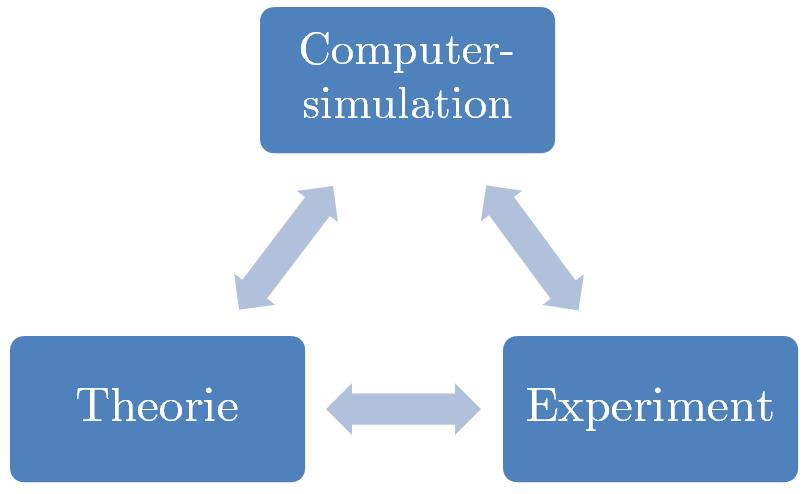
\includegraphics[width=0.45\textwidth]{Null_DrittesStandbein.jpg}
	%\caption{}
	\label{Null_DrittesStandbein}
\end{figure}
\begin{itemize}
\item Vorteile:

\begin{itemize}
\item löst Probleme für die es keine analytische Lösung gibt
\item schafft Raum für Modelle, zu denen es keine analytischen Verfahren gibt
\item kann physikalische Größen berechnen, die nicht messbar sind 
\item immer leistungsfähiger
\item immer billiger
\end{itemize}


\item Vorgehensweise:

\begin{itemize}
\item Modellierung: realistisch $\longleftrightarrow$ einfach
\item Programmierung / Test
\item Erzeugen von Daten / Optimierung
\item Analyse / Interpretation
\end{itemize}
\end{itemize}

\subsection{Hardware}
Diese Vorlesung beschäftigt sich nicht mit Hardware an sich, aber wir müssen abschätzen, ob ein Problem nummerisch lösbar ist! 

\textbf{Beispiel:} Wie weit kann ein Rechner zählen?
\begin{align*}
S(N)= \sum_{i=1}^N x_i \; \mbox{  beispielsweise mit: } x_i = 1
\end{align*}


\begin{enumerate}
\item \textbf{Rechenleistung:} 
typisch 10 GFLOP/S ('\textbf{G}igia \textbf{F}loating \textbf{P}oint \textbf{O}perations \textbf{P}er \textbf{S}econd', Gleitkommazahlen Operationen) \\
\underline{Zum Beispiel Additionen:} \\ %TODO format passt?
Bei $N=10^{10} $ pro Sekunde \\
$\Rightarrow$  Für die Zahl der Atome  ($N = 10^{23}$) dann $10^{13} s \approx 3 \cdot 10^5 a$

\item \textbf{Speicherbedarf:} \\
'Trivialmodell' eines Rechners: 
\begin{center}
\begin{figure}[ht]
	\centering
  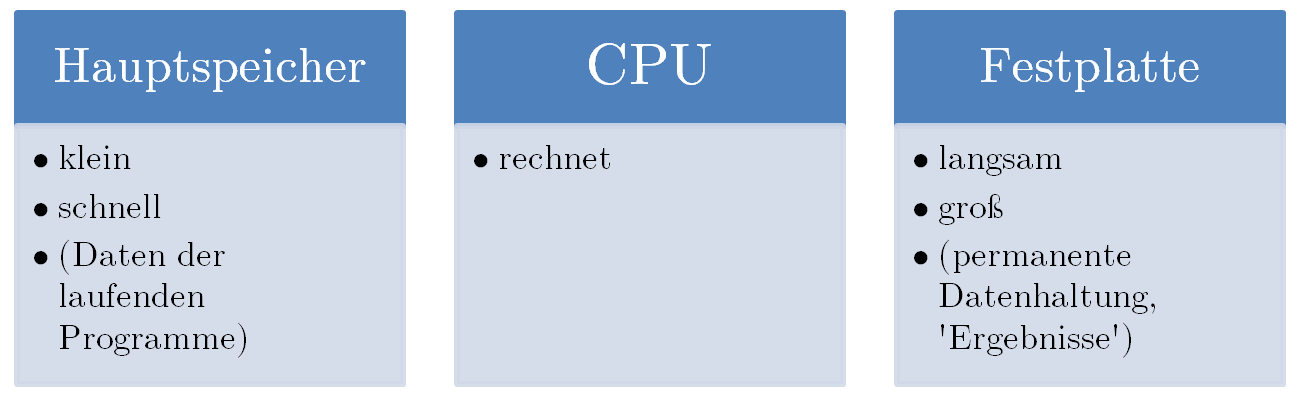
\includegraphics[width=0.8\textwidth]{Null_Rechner.png}
	%\caption{}
	\label{Null_DrittesStandbein}
\end{figure}
\end{center}

Informationseinheit: 
\begin{align*}
 1 Byte \;   \widehat{=} & \; 1 \mbox{ Zeichen (z.B. einer Tastatur)} \\
 1 kByte \; \widehat{=} & \;  1 \mbox{ Seite Text (z.B. 50 Zeilen, 20 Seiten}) 
\end{align*}
Typisch beim Programmieren ist die Gleitkommazahl (\textit{'double'} in C):
\begin{align*}
double \; \widehat{=} \; 8
\end{align*}
\begin{align*}
\Rightarrow 10^{10} \mbox{ Zahlen} \; \widehat{ \approx } \; 10^{11} Byte \; \approx \; 100 \; GB
\end{align*}
Typischer \textbf{Hauptspeicher} (bei uns $16 \; GB$) wäre im Bruchteil einer Sekunde voll. Die Zahlen, die der Rechner in einer Sekunde verarbeitet \textit{passen nicht} in den Hauptspeicher, falls Zwischenergebnisse gespeichert werden (ist aber auch nicht nötig). Eine typische \textbf{Festplatte} fasst $500 \; GB$. Hier passen die Daten drauf. 

\item \textbf{Präzision:} \\

\begin{center}
\begin{tabular}{|c|c|c|}
\hline 
 & \textbf{Integer} (ohne Komma) & \textbf{Double} (mit Komma) \\ \hline
 Wertebereich (min/max) & $\pm 2147 \; 483 \; 647 \approx 2 \cdot 10^9$ & $\pm 2 \cdot 10^{308} $ \\
 Genauigkeit & 1 & $2 \cdot 10^{-16} \widehat{=} 17$ Stellen \\ \hline
\end{tabular} 
\end{center}
Vorsicht - der Computer nähert/rendert! \\
\begin{itemize}
\item Der Wertebereich vom Integer wird nach $0,2 s$ verlassen
\item Der Wertebereich vom Double wird nach $2 \cdot 10^6 s \; \widehat{=} \; 23 d$ verlassen.
\end{itemize}
\textbf{Beispiel:} (Addieren) Wo sind die Grenzen?
\begin{align*}
\sum_{i=1}^N 1
\end{align*}
\begin{enumerate}

\item Wenn alle Partialsummen in ein Feld aufgeschrieben werden, läuft der Hauptspeicher nach spätestens $16/100s$ über.

\item nach $0,2s$ reicht Integer Wertebereich nicht mehr %TODO missing word, 

\item Nach $ 2 \cdot 10^6 s \; \widehat{=} \; 23 d$ reicht Double Präzision nicht \\
(Beispielsweise 17 Stellen: $ 1\; 2 \; 3\; 4\; 5\; 6\; 7\; 8\; 9\; 0 \;1\; 2\; 3\; 4 \; 5 \; 6 +1$ obwohl $10^{18} < 2 \cdot 10^{308}$) \\
 %TODO missing words 

\textbf{Beispiel:} (Addition von Double) \\
5 signifikante Stellen - Berechnung von $10^9 + 10^4$:
\begin{align*}
& \mbox{ \textit{Exakt:} }  \;  && = 1 \cdot 10^9 + 0,00001 \cdot 10^9 = 1,00001 \cdot 10^9 \\
& \mbox{ \textit{Rechner:} }  &&= 1,0000 \cdot 10^9 + 0,0000... \cdot 10^9 = 1 \cdot 10^9
\end{align*}

\underline{Bemerkung:} $\Rightarrow $ 1. Kommutativgesetz der Addition gilt nicht nummerisch! 

Denn:
\begin{align*}
1 \cdot 10^9 + \underbrace{ 0,000001 \cdot 10^9 + ... }_{10^{5}} = 1 \cdot 10^9
\end{align*}
während
\begin{align*}
\underbrace{0,00001 \cdot 10^9 + ... }_{10^5} + 1 \cdot 10^9 = 1,0001 \cdot 10^9
\end{align*}
$\Rightarrow$ Regel für den Programmierer: Bei langen Zahlenreihen erst die kleinen addieren! 
\end{enumerate}
\end{enumerate}

\section{Stochastische Physik}

\subsection{Mikrozustände, Phasenraum und Entropie}
Die \textbf{Gesamtheit (Ensemble)} ist eine Menge von Mikrozuständen, die einen Makrozustand repräsentieren (Zeit/Systemabhängig). Der \textbf{Mikrozustand} eines Systems wird durch generalisierte Koordinaten $q_i$ und Impulse $p_i$ mit $i=\{ 1,...,3N\} $ beschrieben. \\
$\to 6N$-dimensionaler Phasenraum. Ein Punkt im Phasenraum ist ein Mikrozustand, Dynamik führt auf eine Bahn (\textit{Phasenraumtrajektorie)} Siehe Abbildung \ref{fig:Phasenraum}.

\begin{figure}[h]
		\begin{subfigure}[h]{0.5 \textwidth}
		\centering
		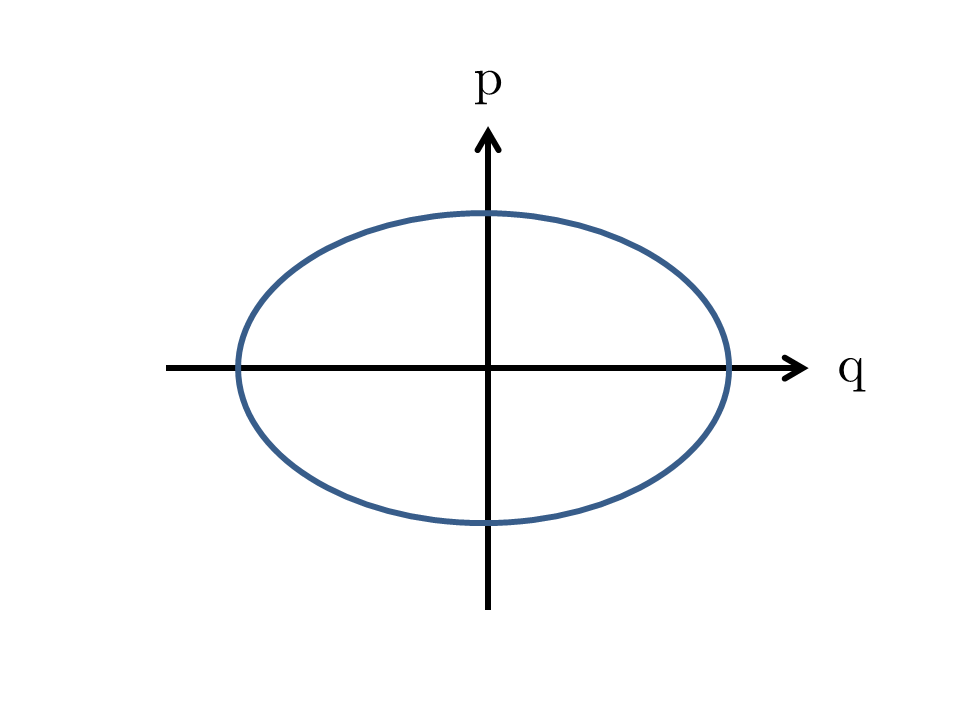
\includegraphics[width=\textwidth]{Folie1.png}
		\caption{Phasenraumtrajektorie des $1d$ harmonischen Oszillators. $q(t) \propto cos( \omega t)$ und $p(t) \propto sin(\omega t)$} 
		\label{fig:Phasenraum}
		\centering
	\end{subfigure}
	~
	\begin{subfigure}[h]{0.5\textwidth}
		\centering
		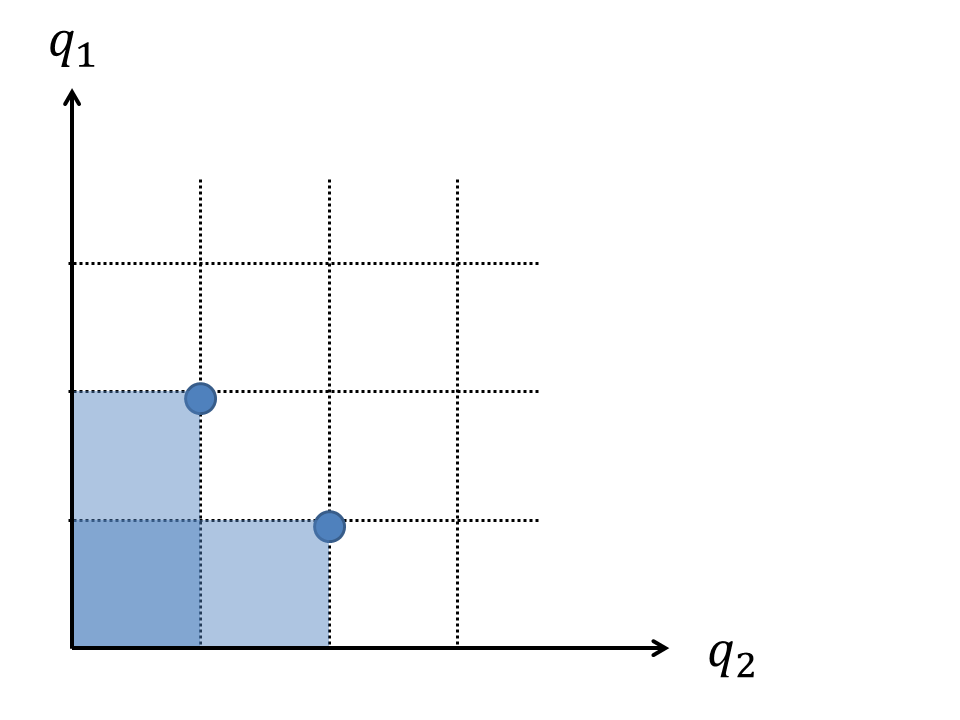
\includegraphics[width=\textwidth]{Folie2.png}
		\caption{Ununterscheidbare Zustände} 
		\label{fig:unterscheidbar}
		\centering
	\end{subfigure}
	\caption{ }
\end{figure}


Die \textbf{Hamiltonfunktion} $H(q,p)$ entspricht der Gesamtenergie des Systems. \textbf{Energieerhaltung:} Im abgeschlossenen System ist die Gesamtenergie konstant mit $U = H (q (t), p(t)) = const.$ (\textit{innere Energie}). \\
Die stochastische Beschreibung ist zurückzuführen auf die \textbf{Wahrscheinlichkeitsverteilung} $\rho (p,q)$\footnote{ besser: eine Wahrscheinlichkeitsdichte} mit der Wahrscheinlichkeit $\rho (q,p) dq^{3N} dp	^{3N}= \prod_{i=1}^{N} \; dq_i dp_i =: d\Gamma $  die Mikroszustände im Phasenraumelement $dq^{3N} dp^{3N} $ des Systems zu finden. Die Normierung verlangt: 
\begin{align}
1 = \int \rho (q,p) \; d\Gamma \mbox{ (mit Phasenraumvolumen } d\Gamma)
\end{align}

Das Phasenraumintegral wird also etwas anders definiert:
\begin{enumerate}
\item Faktor $\frac{1}{h^{3N}}$ wird eingeführt, damit $\rho $ dimensionslos ist. Mit dem \textsc{Planck}schen Wirkungsquantum $h$ und macht Sinn wegen $\Delta q \Delta p \approx h$ (kleinstmögliches Phasenraumelement)
\item Bislang gehen wir davon aus, dass die Teilchen ununterscheidbar sind (durchnummerierbar). Siehe Abbildung \ref{fig:unterscheidbar}. Bei unterscheidbaren Teilchen wäre das gleiche Zustände! Deswegen muss zusätzlich durch die Zahl der Vertauschungen ($N! $) dividiert werden! (\textsc{Gibbson}scher Korrelationsfaktor)
\begin{align}
1 = \frac{1}{h^{3N} N!} \int \rho (q,p)\;  d\Gamma
\end{align}
Ohne diese Korrektur kommt man zum \textsc{Gibb}schen Paradoxon. Der \textbf{thermische Mittelwert} $A(q,p)$ einer beliebigen Größe ist damit

\begin{tcolorbox}[ams gather,title= thermischer Mittelwert, colback=blue!10!white, colframe=blue!30!black] 
 \langle A \rangle = \frac{1}{h^{3N} N!} \int \rho (q,p)\; A(q,p) \;  d\Gamma 
\end{tcolorbox}
Dieser ist Nummerisch nicht lösbar, da für 10 Teilchen bereits $10^{60}$ Rechenoperationen nötig wären! 
\end{enumerate}
Die \textbf{Entropie} definieren wir analog zur Informationstheorie über 
\begin{align}
S = - \langle k_B ln(\rho ) \rangle  = -\frac{k_B}{h^{3N} N!} \int \rho \; ln(\rho ) d\Gamma 
\end{align}
Bedeutung der Entropie: 
\begin{itemize}
\item Informationsgehalt und Ungewissheit (\textit{Informationstheorie});
\item  thermisches Mittel, 'Unordnung' (\textit{Physik})
\end{itemize}  

\textbf{Beispiel:} (gezinkter Münzwurf)\\
Es sei $p(Kopf) = p \neq p(Zahl)= q$ und $1=p+q$. %TODO zweimal gleiches P? oder Pp?
\begin{align*}
\Rightarrow S =& - k_B \underbrace{\sum_{_{Kopf, Zahl}} \rho \; ln(\rho ) }_\text{Integral wird Summe} = -k_B  (p \; ln(p) + q \; ln(q)) \\
=&  -k_B ( p \; ln(p) + (1-p) \; ln(1-p))
\end{align*}
Wir werfen N-mal: (siehe Abbildung \ref{fig:Bogen})

\begin{figure}[h]
		\begin{subfigure}[h]{0.5 \textwidth}
		\centering
		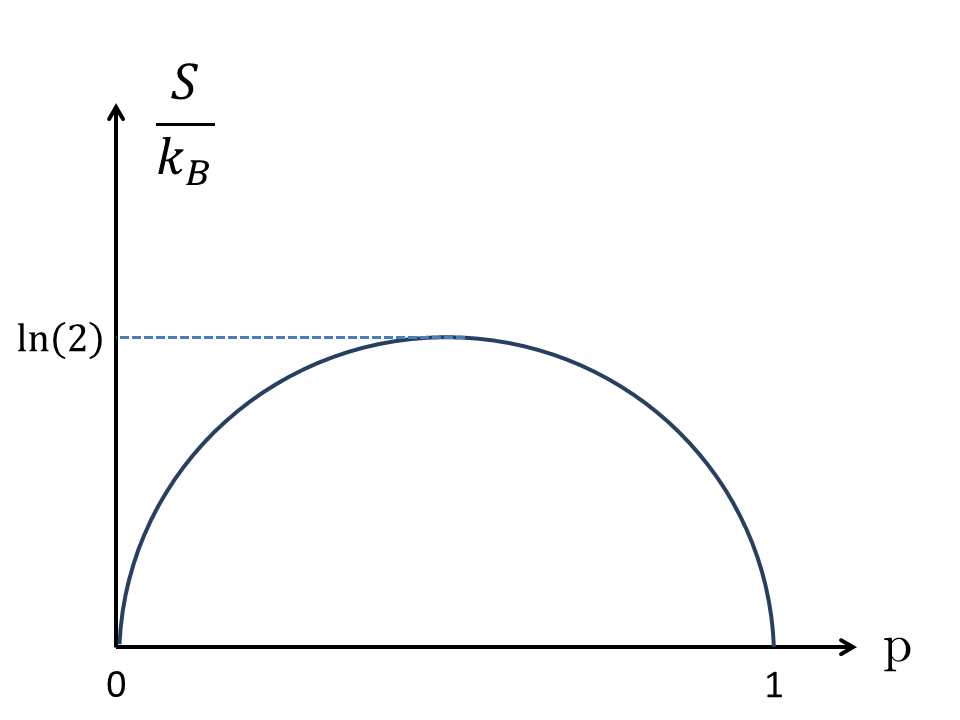
\includegraphics[width=\textwidth]{Folie3.png}
		\caption{(Gezinkter) Münzwurf} 
		\label{fig:Bogen}
		\centering
	\end{subfigure}
	~
	\begin{subfigure}[h]{0.5\textwidth}
		\centering
		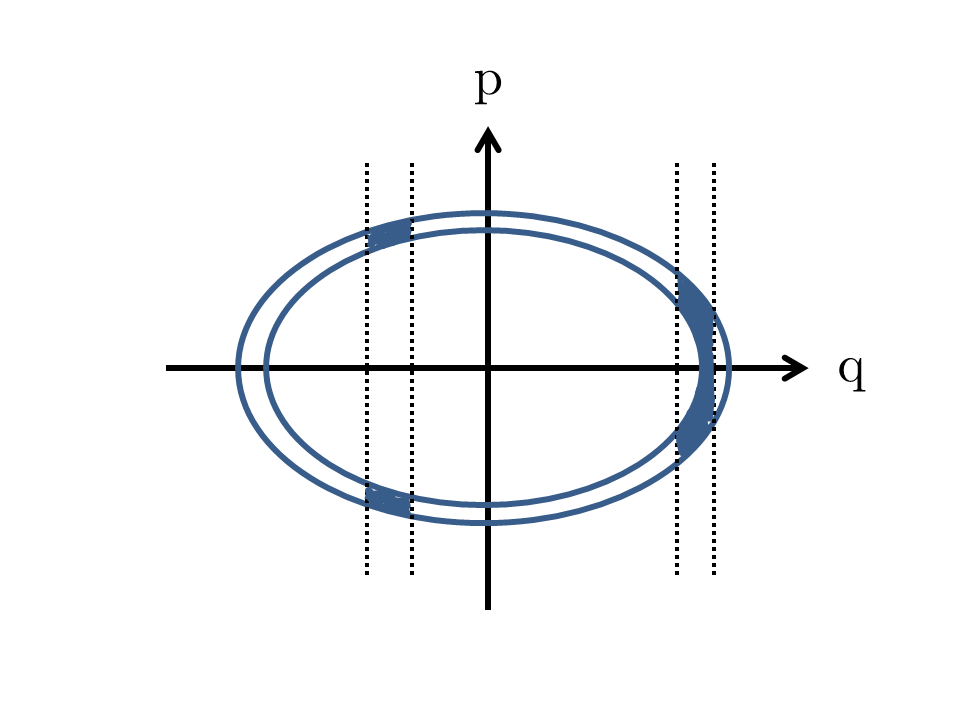
\includegraphics[width=\textwidth]{Folie4.png}
		\caption{Hyperfläche} 
		\label{fig:Trajektorie}
		\centering
	\end{subfigure}
	\caption{ }
\end{figure}

\begin{align*}
\begin{rcases}
p= 0: Z\; Z\; Z\; Z\; Z\; Z\; Z\; ... \\ 
p= 1: K\; K\; K\; K\; K\;  ...  
\end{rcases}
\text{ 'Unordnung', 'Informationsgehalt' S = 0} \\
\end{align*}
\begin{align*}
\begin{rcases}
p= 0.5: K\; K\; Z\; K\;  Z\; ...
\end{rcases}
\text{S maximal}
\end{align*}
Im Phasenraum: $S=0$ bestehen überall $\rho = 0$ außer an einem Punkt $\rho(p_0, q_0) = 1$ $\Rightarrow$ nur \textit{ein} Mikrozustand zu vorgegebenen Makrozustand. Hohe Entropie heißt, viele, gleich wahrscheinliche Mikrozustände. 

\subsection{Mikrokanonische Gesamtheit}
\textbf{Ziel allgemein:} Bestimmung von $\rho$ für definierte physikalische Systeme \\
\underline{Hier (mikrokanonisch):} Isoliertes (abgeschlossenes) System mit festem $U,V,N$ (innere Energie, Vauum, Teilchenzahl). \footnote{Zur Erinnerung: \\ Die \textit{kanonische} Gesamtheit: festes N, Energiefluktuation\\ Das\textit{ großkanonische} Ensemble: Energie- und Teilchenfluktuation}

Wir postulieren, dass dann $\rho$ für alle erlaubten Zustände gleich ist, also
\begin{align}
\rho (q,p) = 
\begin{cases}
\rho  & \mbox{ für } H(p,q) = U \\
0 & \mbox{ sonst }
\end{cases}
\end{align}
Da $\rho $ Volumenintegral, ist es zweckmäßig, Volumen zwischen zwei Hyperfllächen zu betrachten (siehe Abbildung \ref{fig:Trajektorie}):
\begin{align}
\beta = \{ (p,q): U \leq H (p,q) \leq U +\Delta \}
\end{align}
später dann $\Delta \to 0$. 
\begin{align}
\int_\beta \underbrace{ \; d \Gamma }_{ inkl.  \; (h^{3N} N!)^{-1}  } = 1 \; \Rightarrow \rho = \frac{1}{Z}
\end{align} 

mit der \textbf{Zustandssumme der mikrokanonischen Gesamtheit}
\begin{align}
Z_\Delta = \int_\beta d\Gamma = Z_\Delta (U,V,N) 
\end{align} \footnote{U steht in $\beta$, V steckt in $d\Gamma$, N steckt in Dimension des Phasenraums. Z ist eine thermodynamische Größe. Im mikrokanonischen Ensemble führt Z auf S.}
\begin{align}
\Rightarrow S =& - \langle k_B \rho \; ln(\rho ) \rangle = - k_B \underbrace{\int_\beta d\Gamma \rho \; }_{=1} \underbrace{ln(\rho)}_\text{unabhängig von p,q} \\
=& k_B ln (Z_\Delta(U,V,N)) \\
=& - k_B \; ln(\rho )
\end{align}

Zusammenhang zur Thermodynamik: S(U,V,N) ist ein thermodynamisches Potential mit natürlichen Variablen U,V,N
\begin{align}
\begin{rcases}
& \frac{\partial S}{\partial U} \biggr\vert_{V,N} = \frac{1}{T} = k \frac{1}{Z} \left( \frac{\partial Z}{\partial U}\right)_{V,N} \\
& \frac{\partial S}{\partial V} \biggr\vert_{U,N} =  -\frac{p}{T} \\
& \frac{\partial S}{\partial N} = \frac{\mu }{T}
\end{rcases}
 dS = \frac{\partial S}{\partial U} dU +\frac{\partial S}{\partial V}dV+  \frac{\partial S}{\partial N} dN
\end{align}

Abschließende Bemerkungen: 
\begin{itemize}
\item Zustandssumme der mikrokanonischen Gesamtheit kann als 'Zahl der Zustände' zu vorgegebener Energie U interpretiert werden: 
\begin{align}
Z = \frac{1}{h^{3N} N!} \int_{H(p,q)=U} dp \; dq
\end{align}
also Entropie $\propto ln(\mbox{Zahl der Zustände})$
\item Rechnungen in der mikrokanonischen Gesamtheit sind recht kompliziert wegen der Randbedingung $H=U$. Besser sind andere Gesamtheiten. 
\item Statistik erfordert den Limes großer Teilchenzahlen
\end{itemize}
\textbf{Wichtig: löst man nummerisch Bewegungsgleichnungen unter Energieerhaltung, summiert man im mikrokanonischen Ensemble}
\subsection{Kanonisches Ensemble}

\begin{figure}[h]
		\begin{subfigure}[h]{0.5 \textwidth}
		\centering
		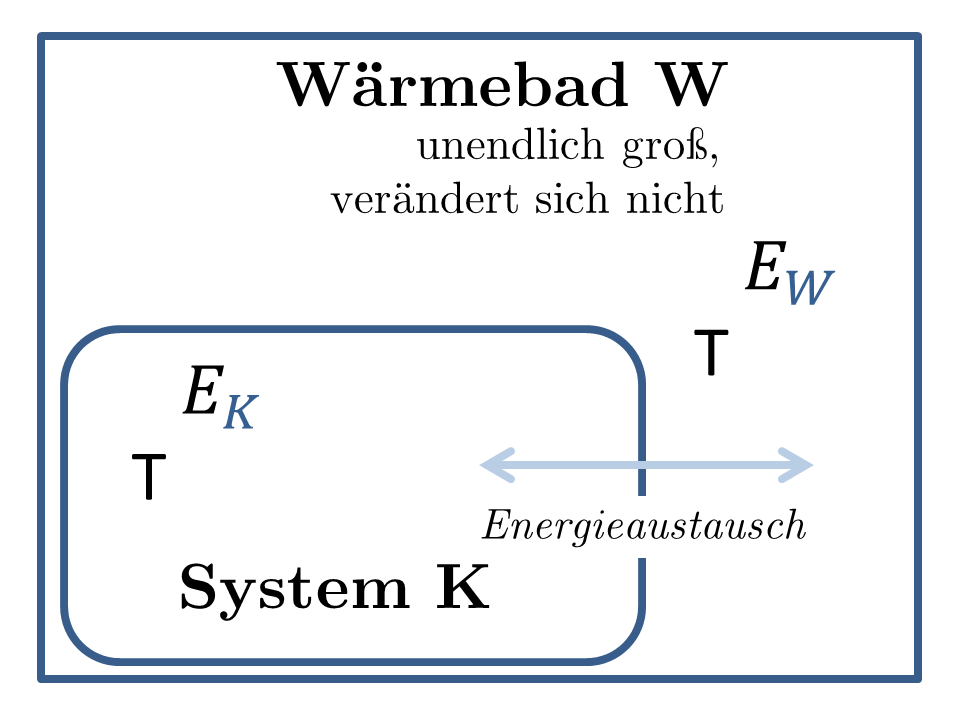
\includegraphics[width=\textwidth]{Folie5.png}
		\caption{kanonische Gesamtheit} 
		\label{fig:Waermebad}
		\centering
	\end{subfigure}
	~
	\begin{subfigure}[h]{0.5\textwidth}
		\centering
		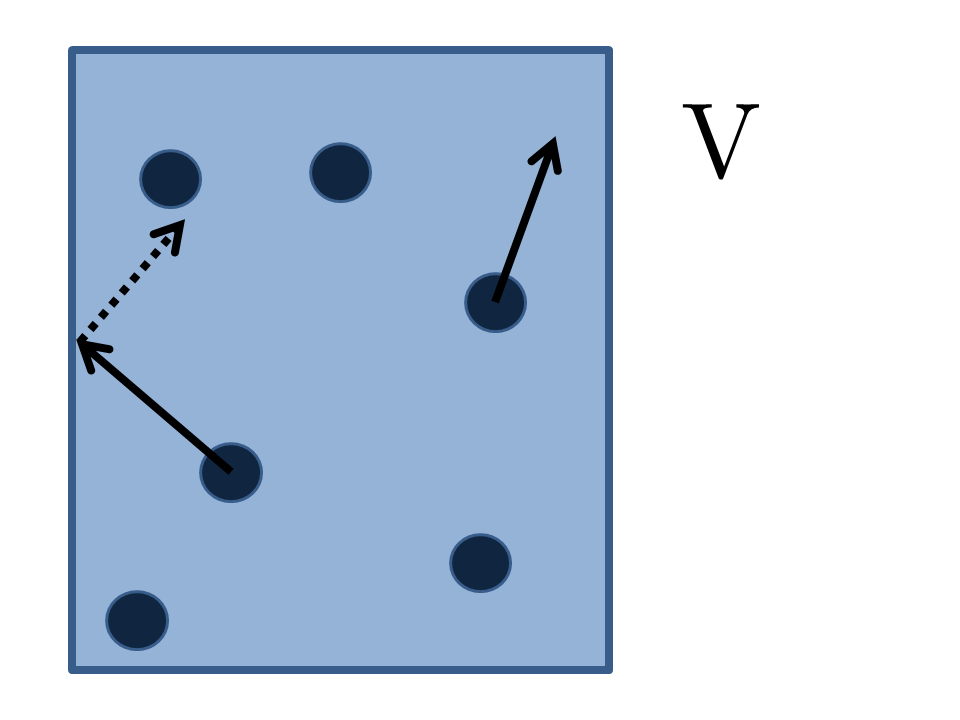
\includegraphics[width=\textwidth]{Folie6.png}
		\caption{Volumenbegriff, ideales Gas} 
		\label{fig:Volumen}
		\centering
	\end{subfigure}
	\caption{ }
\end{figure}

Wir betrachten jetzt ein System in Kontakt mit einem Wärmebad der Temperatur $T$, gemäß Abbildung \ref{fig:Waermebad}. \\



\begin{itemize}
\item Die Gesamtenergie $E = E_w + E_k$. \\
\item Das Wärmebad soll sehr groß sein, sodass $\frac{E_K}{E} << 1$
\item Die Energie in K ist nicht mehr Konstanz, nur im Gesamtsystem. Das Gesamtsystem ist mikrokanonisch, alle Gesamtzustände sind gleich wahrscheinlich. Gesucht ist die Wahrscheinlichkeitsdichte $\rho (p,q) = \rho_i $ der Mikrozustände in K. 
\item $\rho_i$ gehört zum Mikrozustand mit Energie $E_i$ (siehe links) %TODO what? LEft? 
Zahl der Makrozustände des Gesamtsystems ist gleich der Zahl der Mikrozustände des Wärmebads mit $E_w = E - E_i$ (bzw. gleich der mikrokanonischen Zustandssumme) 
\begin{align}
Z_w (E- E_i): \rho_i \propto Z_w (E-E_i)
\end{align}
Betrachte Entropie
\begin{align}
S_w &= k_B ln (Z_w (E-E_i)) \\
&= k_B ln (Z_w (E)) - \underbrace{ k_B \frac{\partial ln (Z_w (E-E_i))}{\partial E_i}}_{ \frac{1}{T}} E_i \; ( E >> E_i) \\
& \Rightarrow Z_w (E-E_i) = Z_w (E) e^{-\frac{E_i}{k_B T}} \\
&\Rightarrow \rho_i \propto e^{- \frac{E_i}{k_B T} } \; \mbox{  ('\textsc{Boltzmann}-Faktor')} \\
&\Rightarrow \rho (p,q) \propto e^{- \beta \; H(p,q)} \; \mbox{ mit: } \beta = \frac{1}{k_B T}
\end{align}
Die Normierung von $\rho$ verlangt: 
\begin{align}
\rho (p,q) = \frac{e^{- \beta \; H(p,q)}}{Z}
\end{align}
mit
\begin{align}
Z = \int d \Gamma e^{- \beta \; H(p,q)}
\end{align}
der \textbf{Zustandssumme der kanonischen Gesamtheit.} Integral erstreckt sich über den gesamten Phasenraum. \textbf{Thermodynamik:}
\begin{align}
S &= -k_B \int d\Gamma \rho \; ln(\rho ) = -k_B \int d\Gamma \frac{e^{- \beta \; H}}{Z} (- \beta H - ln(Z)) \\
&= \frac{1}{T} \underbrace{ \int d\Gamma \; H \; \rho}_U + k_B ln(Z) \int d\Gamma \; \rho \\
&=\frac{U}{T} + k_B ln(Z)
\end{align}
\begin{align}
&\Rightarrow TS = U + k_B T ln(Z) \; (F= U - TS) \\
& \Rightarrow \mbox{ Freie Energie: } F = - k_B T ln(Z) = F(T,V,N)
\end{align}
\textbf{Beispiel:} (Ideales Gas, gemäß Abbildung \ref{fig:Volumen})
\begin{align*}
H = \sum_{i=1}^N \frac{p_i ^2}{2m} \; ,  \; \mathbf{p_i} = (p_x, p_y, p_z)
\end{align*}
Kanonische Zustandssumme
\begin{align*}
Z(T,V,N) &= \frac{1}{h^{3N} N!} \int d\Gamma e^{- \beta \sum \frac{p_i ^2}{2m} } = \frac{V^N}{h^{3N} N!} \int dp_1 ^3 ...dp_N ^3 \;  e^{ - \beta \frac{p_1 ^2}{2m}} ... e^{- \beta \frac{p_N ^2}{2m}}  \\
&=  \frac{V^N}{h^{3N} N!} \; \prod_{i=1}^N \underbrace{\int dp_i ^3 \; e^{- \beta \frac{p_i ^2}{2m}} }_{ \sqrt{\frac{2m\pi}{\beta}}} \tag{$i = 1...N$ Teilchen} \\
&= \frac{V^N}{h^{3N} N!} \; \prod_{i=1}^{3N}  \int dp_i  \; e^{- \beta \frac{p_i ^2}{2m}} \tag{$i = 1...3N,$  N Teilchen mit $(x,y,z)$} \\
&= \frac{V^N}{h^{3N} N!} \sqrt[\frac{3N}{2}]{\frac{2m\pi}{\beta}}
\end{align*} %TODO alle p_i Vektoren?
\end{itemize}
Für die freie Energie verwenden wir die \textsc{Stirling}-Formel für große N:
\begin{align}
ln(N!) \approx N \; ln(N) - N
\end{align}
\begin{align}
\Rightarrow F = -k_B T \; ln(Z) = -k_B T N \left[ ln \left(\frac{V}{N}\right) + \frac{3}{2} ln \left(\frac{2 m \pi }{h^3} k_BT \right) +1 \right]
\end{align}

\begin{align}
\Rightarrow p = - \frac{\partial F}{\partial V} \biggr\vert_{T,N} = \frac{N k_B T}{V}
\end{align}

\begin{tcolorbox}[ams gather,title= ideale Gasgleichung, colback=blue!10!white, colframe=blue!30!black] 
 p V = N k_B T
\end{tcolorbox}

Es folgt also eine der Gasgleichungen. Die andere folgt aus
\begin{align}
U = F + TS = F + T \frac{\partial F}{\partial T} \biggr\vert_{V,N} = \frac{3}{2} N k_B T
\end{align}
\textbf{Diskussion:} \\
\begin{itemize}
\item gilt auch für großkanonische Gesamtheiten
\item Berechnung zu verschiedenen Gesamtheiten führen zu gleichen thermodynamischen Potentialen (also 'gleichen Ergebnissen'). $\to$ Nach \textsc{Legendre}-Transformation, Zustandssummen verschieden. \\
Rechnungen jedoch verschieden, Numerik auch! (z.B. Resultate) %TODO stimmt resultate?
\item Phasenraumintegrale werden meist nicht numerisch berechnet %TODO ?? Stimmt der satz?
(\textit{Ausblick:} MD, MC) 
\end{itemize}
\subsection{Weitere Resultate der statistischen Mechanik}
\begin{itemize}
\item \textbf{Extremalprinzip:} im Gleichgewicht werden thermodynamische Potentiale extremal\footnote{genau genomme wir $\rho$ so gewählt}, z. B. 
\begin{align}
& S(U,V,N) \, && \mbox{ maximal} \\
& F(T,V,N), \; U(S,V,N) \; && \mbox{ minimal}
\end{align}
\item \textbf{Schwankungen:} Die Wärmekapazität
\begin{align}
c_v = T \frac{\partial ^2 U}{\partial S ^2} \biggr\vert_{V,N} = \frac{\partial U}{\partial T}  \biggr\vert_{V,N} &= \frac{1}{k_B T^2} \langle (H - \langle H \rangle)^2\rangle \\
&= \frac{1}{k_B T^2} \left( \langle H^2 \rangle - \langle H \rangle ^2 \right) \mbox{ (numerisch geschickt)}
\end{align}
\item \textbf{Gleichverteilungssatz:} jede quadratische Form in H gibt einen Beitrag $\frac{k_B T}{2}$ in U. 
\textbf{Beispiel:} (ideales Gas) 
\begin{align*}
H = \sum_{i=1}^N \frac{p_i ^2}{2m}
\end{align*}
mit $p^2 = p_x^2 + p_y^2 + p_z^2 \Rightarrow U= \frac{3}{2} N k_B T$ (gut für Tests der Numerik) 
\end{itemize}

\section{Monte Carlo Verfahren}
\subsection{Zufallszahlen}
Statistik wichtig für Physik und andere Disziplinen. Physikalische Probleme sind oft ähnlich. Statt beispielsweise$10^{23}$ Atomen werden nur wenige betrachtet, dann 'hochgerechnet'.  \\
$\Rightarrow$ Zahl der Freiheitsgrade sinnvoll beschränken. Häufig wichtig für 'Stichprobe': zufällige Auswahl  $\to$ also Zufallszahl.\\
Im einfachsten Fall: \textit{diskrete Zufallszahlen} $x_1 ... x_N$\\

\begin{figure}[h]
		\begin{subfigure}[h]{0.5 \textwidth}
		\centering
		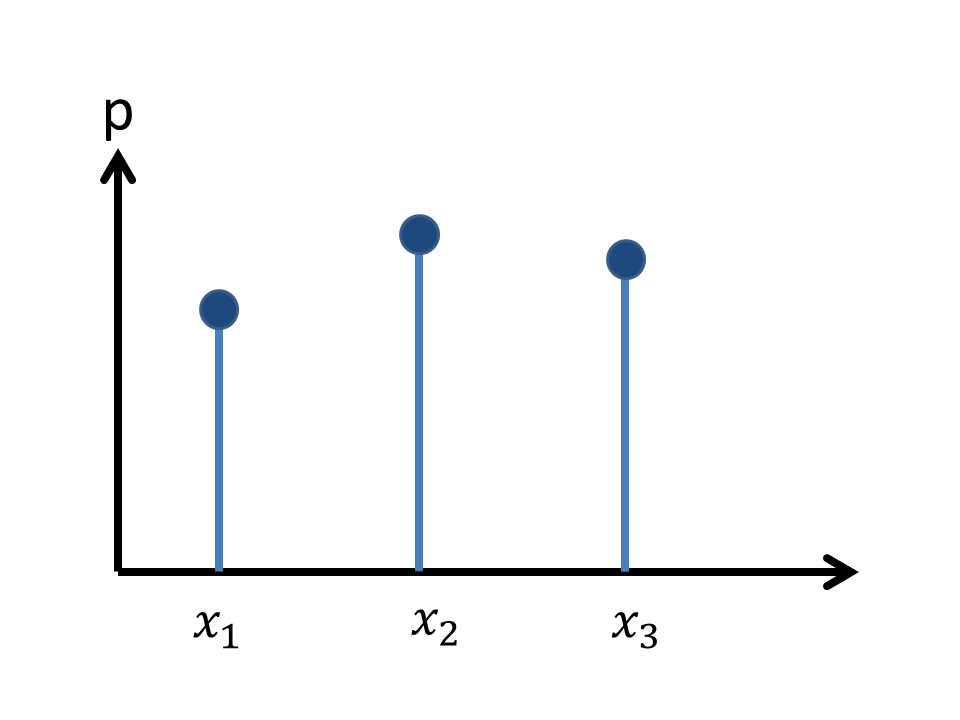
\includegraphics[width=\textwidth]{Folie7.png}
		\caption{Würfelwurf} 
		\label{fig:Wuerfelwurf}
		\centering
	\end{subfigure}
	~
	\begin{subfigure}[h]{0.5\textwidth}
		\centering
		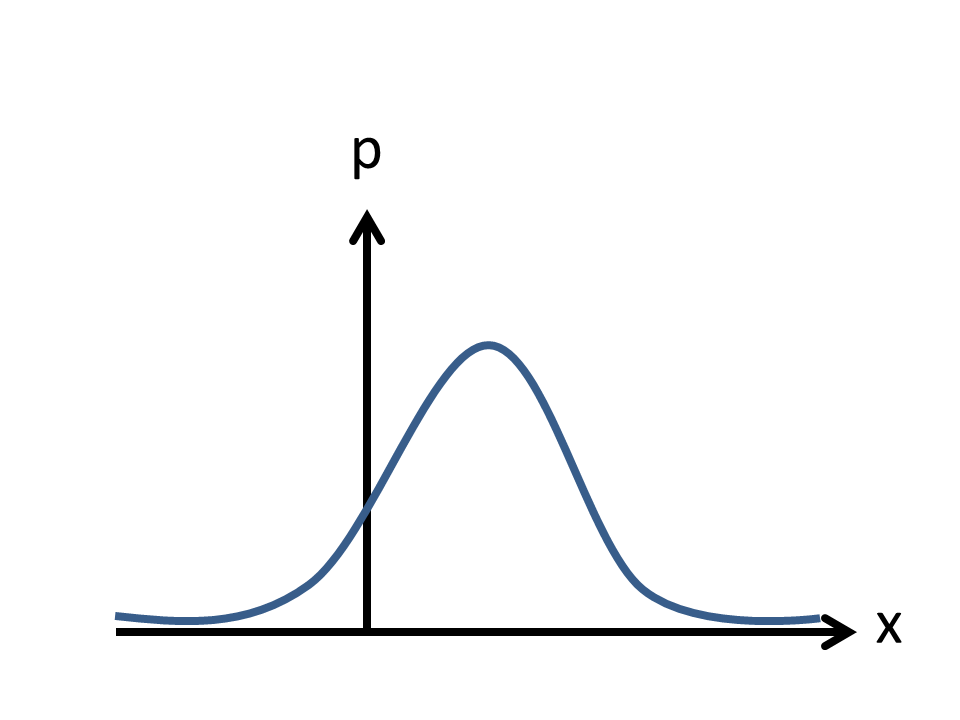
\includegraphics[width=\textwidth]{Folie8.png}
		\caption{kontinuierliche Verteilung von $p(x)$: Die Wahrscheinlichkeitsdichte} 
		\label{fig:wahrscheinlichkeitsdichte}
		\centering
	\end{subfigure}
	\caption{ }
\end{figure}


\textbf{Beispiel:} (Würfel, Abbildung \ref{fig:Wuerfelwurf})  \\
\begin{align*}
x_1 = 1 , \; ... \; ,  x_6 = 1 , \; (N=6)
\end{align*}
Die \textbf{Wahrscheinlichkeitsdichte} ist definiert über die
\begin{align}
p_i = \frac{\mbox{Häufigkeit für Auftreten von } x_i}{\mbox{Gesamtzahl der Messungen}} = \frac{m_i}{M} \biggr\vert_{M \to \infty}
\end{align}
\begin{align*}
\sum_{i=1}^N p_i = 1
\end{align*}
\textbf{Beispiel:} (zurück zum Würfel)
\begin{align*}
p_i = \frac{1}{6}, \; i=\{1,...,6\}
\end{align*}
Der \textbf{Mittelwert} ist definiert über
\begin{align}
\overline{x} = \sum_{i=1}^N p_i \; x_i \; = \sum_{i=1}^N \frac{M_i x_i}{M} \biggr\vert_{M \to \infty}
\end{align}
und entsprechend bei kontinuierlicher Verteilung $p(x)$ die 'Wahrscheinlichkeitsdichte' (siehe Abbildung \ref{fig:wahrscheinlichkeitsdichte})
\begin{align}
p(x) \; dx \; = \frac{dM_x}{M}
\end{align}
Normierung:
\begin{align}
\int dx \; p(x) = 1 
\end{align}
\begin{align}
\overline{x}= \int dx \; p(x) \; x
\end{align}
\textbf{Schwankung}
\begin{align}
\overline{(\Delta x)^2} = \sum_{i=1}^N p_i \left( x_i - \overline{x} \right) ^2 \widehat{=} \int dx \; p(x) \; (x- \overline{x})^2
\end{align}
häufig wichtig ist auch

\begin{align}
\overline{(x-\overline{x})^2} = \overline{x^2 - \underbrace{2 \overline{x} x}_\text{=0, s.u.} - \overline{x}^2} = \overline{x^2} - \overline{x}^2
\end{align}  \footnote{mittelt sich zu Null, da nach oben gleiche Abweichung wie nach unten} \\

\begin{figure}[h]
		\begin{subfigure}[h]{0.5 \textwidth}
		\centering
		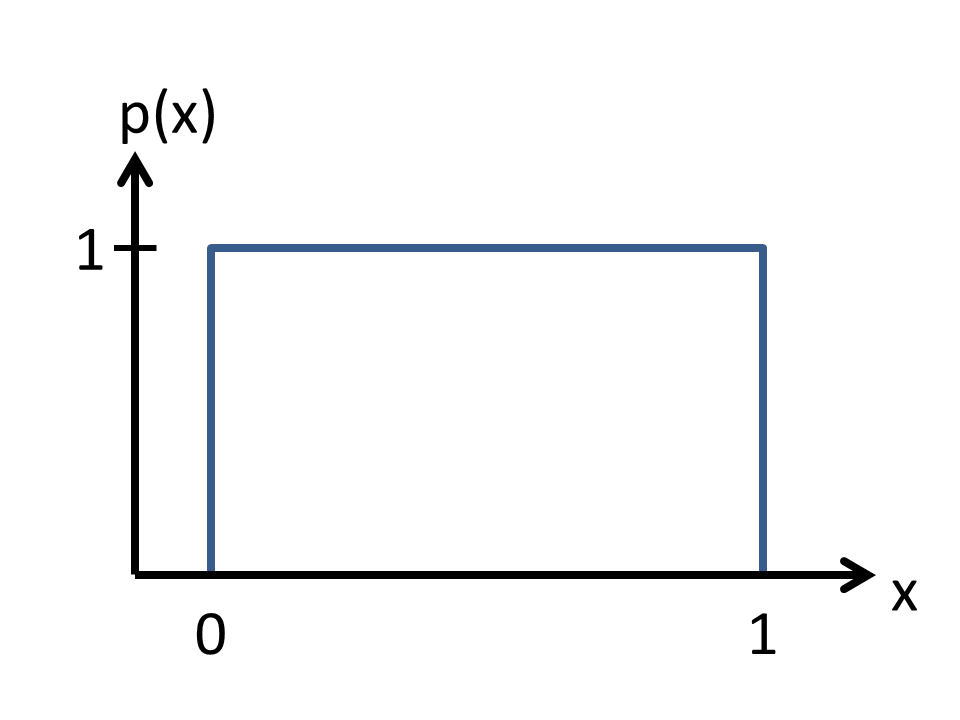
\includegraphics[width=\textwidth]{Folie9.png}
		\caption{Gleichverteilung} 
		\label{fig:Gleichverteilung}
		\centering
	\end{subfigure}
	~
	\begin{subfigure}[h]{0.5\textwidth}
		\centering
		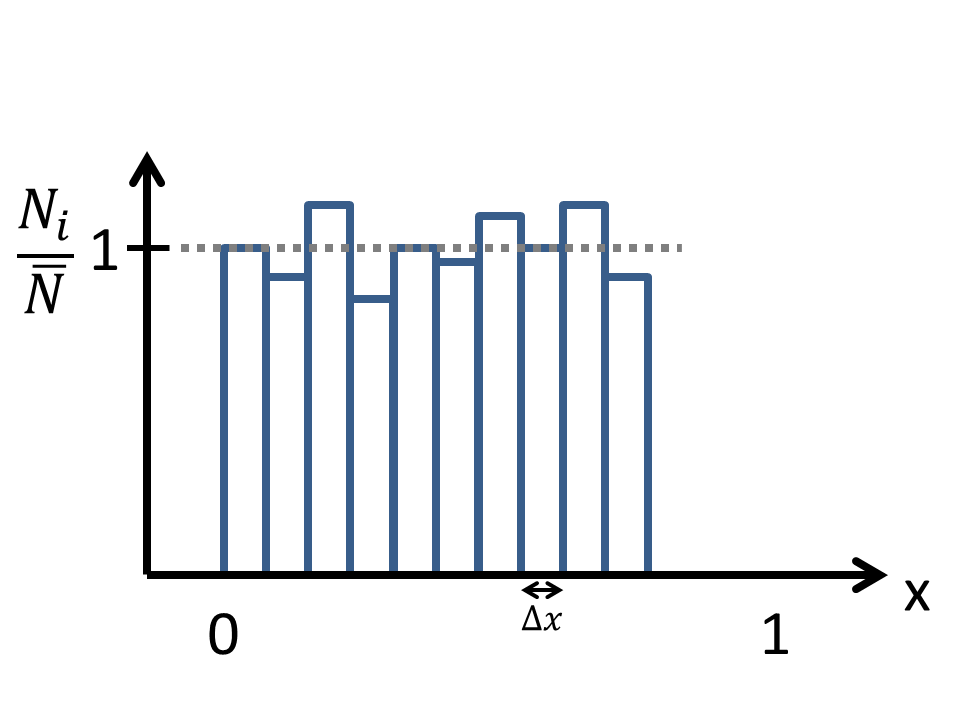
\includegraphics[width=\textwidth]{Folie11.png}
		\caption{Teilintervalle im Wertebereich} 
		\label{fig:Teilintervall}
		\centering
	\end{subfigure}
	\caption{ }
\end{figure}

\textbf{Beispiel:}(Gleichverteilung, Abbildung \ref{fig:Gleichverteilung}) 
\begin{align*}
p(x) = 
\begin{cases}
1  \quad \quad 0 \leq x \leq 1 \\
0  \quad \quad  \text{sonst}
\end{cases}
\quad \Rightarrow \overline{x}= \int_0^1 dx \; x = \frac{1}{2}
\end{align*}
\begin{align*}
\overline{(\Delta x)^2} = \int_0^1 dx \; (x-\frac{1}{2})^2 \approx  \int_0^1 dx \; (x^2-\frac{1}{4}) = \frac{1}{3} - \frac{1}{4} = \frac{1}{12}   \label{Anmerkung}
\end{align*} \footnote{Die Wurzel aus (\ref{Anmerkung}) wäre der Wert für die Breite }
\paragraph{Erzeugung von Zufallszahlen im Rechner}
...geht nicht, da es beim Rechner, einer deterministischen Maschine, keinen Zufall gibt. $\Rightarrow$ 'Pseudo-Zufallszahlen', deterministische Kette von Zahlen $x_i$, die bestimmten Anforderungen genügen: 
\begin{itemize}
\item definierter Wertebereich, \textbf{z.B.} $ [ 0,1] $ \textit{(double)}, $[ 0: RAND\_ \; MAX]$\textit{(Integer)}
\item wohldefinierte Wahrscheinlichkeitsverteilung, gleichverteilt (Abb. \ref{fig:Gleichverteilung}) \textbf{ z.B.} %TODO image doppeltes
\item lange Periode: $x_i$ ist immer periodisch denn
\begin{itemize}
\item Rechner speichert Information
\item Speicher begrenzt $\Rightarrow$ endliche Zahl von Zuständen
\end{itemize}
\item $x_i$ deterministisch $\Rightarrow$ aus \textit{einem} (gleichen) Zustand folgt immer die gleiche Kette $\Rightarrow \; x_i$ sind periodisch
\item großer Wertevorrat (nicht immer nötig) jedoch unmöglich, deshalb Periode lang,\textbf{ z.B.} 1 von N %TODO
aussuchen
\item keine Korrelation, d.h. kein 'einfacher' Zusammenhang zwischen den $x_i$, \textbf{ z.B.}
\begin{align*}
x_{i+k} = x_i 
\end{align*}
geht nicht wegen der Periode (hier wäre die Periode $k$).
\end{itemize}
\paragraph{Methode 1} 

linear konvergente Zufallsgeneratoren \footnote{Anmerkung: Der Rest bei Ganzzahldivision $mod$ $\widehat{=}$ $\% $ in C!} 
\begin{align}
& x_{i+1}= (a x_i + b)\; mod \; m \quad \\
\end{align}
 $x_i$: Integer ,  $m$: Wertebereich und $a,b$: 'magischen Zahlen'. \\
Man kann zeigen: Der Algorithmus hat keine Zyklen $< m$ wenn:
\begin{enumerate}
\item $b$ und $m$ teilerfremd
\item $a-1$ ein Vielfaches von jedem Primfaktor von $m$
\item $a-1$ ein Vielfaches von 4, falls 4 Teiler von $m$
\end{enumerate}
\textbf{Beispiele:} \begin{itemize}
\item $a= 137, \; \quad b= 187, \quad \quad m=256$
\item $ a= 1366, \quad b=150887, \; m=714025$
\end{itemize}
Mögliche Testverfahren dafür sind:
\begin{enumerate}
\item Histogramm bezüglich Gleichmäßigkeit der Verteilung: Man teilt den Wertebereich in $I$ Teilintervalle der Länge $\Delta x$. Es gilt $I \cdot \Delta x = 1$.  Ziehe N Zufallszahlen, $N_i$ im Teilintervall $i$, siehe Abbildung \ref{fig:Teilintervall}.
\begin{align}
N = \sum _{i=1}^I N_i, \quad \quad \quad \overline{N_i} = \frac{N_i}{I}= N \Delta x
\end{align}
\begin{itemize}
\item $\frac{N_i}{N}$ sollte für $N \to \infty $ gegen $\frac{N}{I}$ gehen
\item Konvergenz (Fehler) %TODO FELDER? \\
Betrachte 1. Teilintervall (als Beispiel) Wahrscheinlichkeit, dass von N Zufallszahlen $N_1$ im 1. Teilintervall sind:

\begin{figure}[h] %TODO %TODO IMAGE MISSING! S.59
		\begin{subfigure}[h]{0.5 \textwidth}
		\centering
		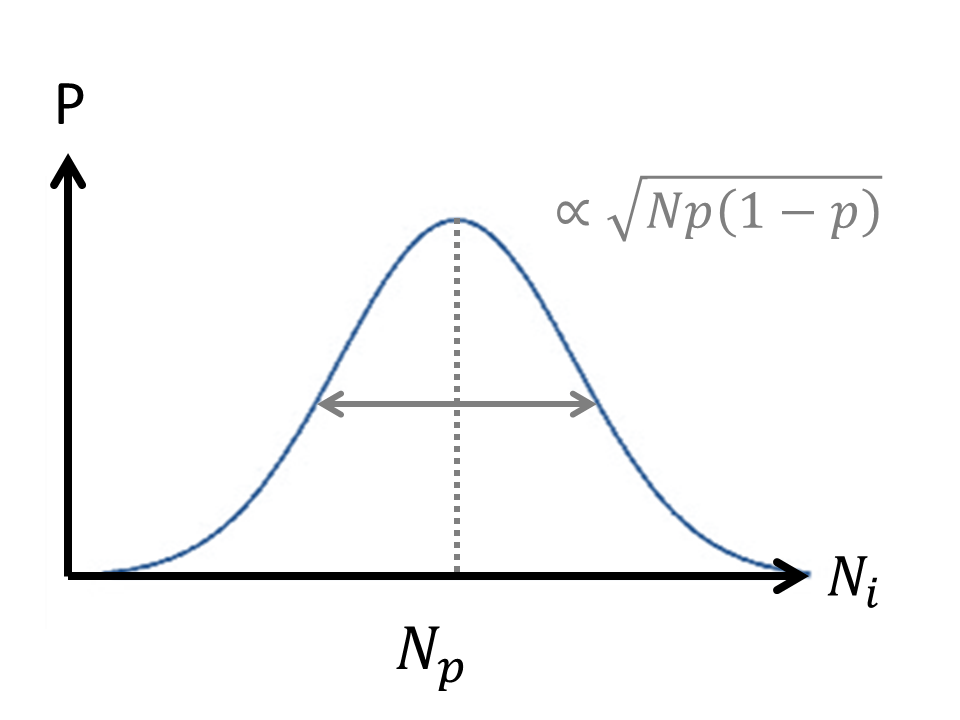
\includegraphics[width=\textwidth]{Folie12.png}
		\caption{Binomialverteilung} 
		\label{fig:Binomialverteilung}
		\centering
	\end{subfigure}
	~
	\begin{subfigure}[h]{0.5\textwidth}
		\centering
		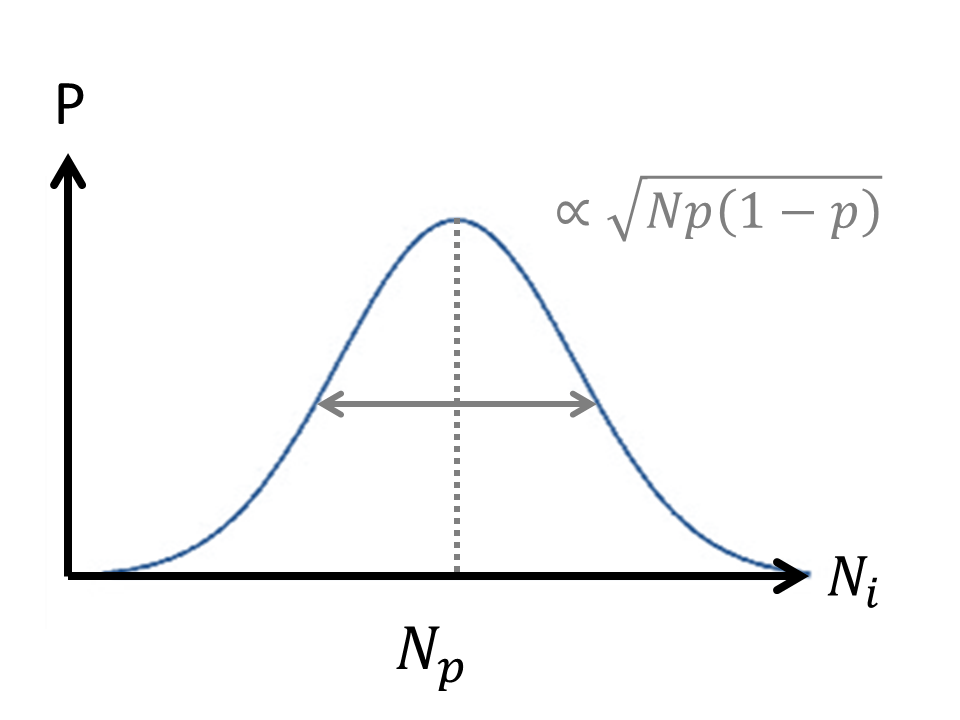
\includegraphics[width=\textwidth]{Folie12.png}
		\caption{\textsc{Gauß}-Funktion} 
		\label{fig:Gaussfunktion}
		\centering
	\end{subfigure}
	\caption{ }
\end{figure}
Anschauliche Darstellung, siehe Abbildung \ref{fig:Binomialverteilung}.
\begin{align}
p_N (N_1) = p^{N_1} (1-p)^{N-N_1} \frac{N!}{N_1 ! (N-N_1)!} \quad  \mbox{ \textbf{'Binomialverteilung'}} \\
 \mbox{ mit } p= \Delta x
\end{align}

Die Binomialverteilung geht in Grenzfällen in einfachere, d.h. analytische Verteilungen über: In diesem Beispiel geht sie für $N \to \infty$ und konstantes $p$ in die \textbf{\textsc{Gauss}verteilung} über.
\begin{align}
p_N (N_1) = \frac{1}{\sqrt{2 \pi N p (1-p)}} e^{- \frac{(N_1 - N_p)^2}{2 N_p (1-p)}}
\end{align}
Der Beweis hierfür ist etwas komplizierter, unter Anderem mit \textsc{Stirling}-Formel $ln(N!) = N \; ln(N) - N + \frac{1}{2} \; ln( 2 \pi N)$. \\
Die Eigenschaften der \textsc{Gauß}-Funktion, siehe auch Abbildung \ref{fig:Gaussfunktion}, auf einen Blick:
\begin{itemize}
\item Mittelwert: $\overline{N_1}= N_p$
\item Schwankung: $\chi ^2 = \overline{(N_1 - \overline{N_1})^2} \propto N p (1-p)$ 
\item $\Rightarrow$ relativer Fehler: $\frac{\sqrt{\chi ^2}}{\overline{N_1}} \propto \frac{\sqrt{N}}{N} \propto \frac{1}{\sqrt{N}}$ 
\end{itemize}
\end{itemize}
\item Weiteres Testverfahren: \\
Auf Korrelation prüfen. Aufeinanderfolgende Zufallszahlen werden als Punkte in einem d-dimensionalen Einheitskubus dargestellt:
\begin{align}
(x_k, x_{k+1}, \; ...\; ,\; x_{k+(d-1)}) \in \mathbb{R}^d
\end{align}
Falls Korrelation vorhanden: Punkte füllen nicht den Raum sondern liegen auf $(d-1)$-dimensionalen Ebenen. \\

\begin{figure}[h] 
		\begin{subfigure}[h]{0.5 \textwidth}
		\centering
		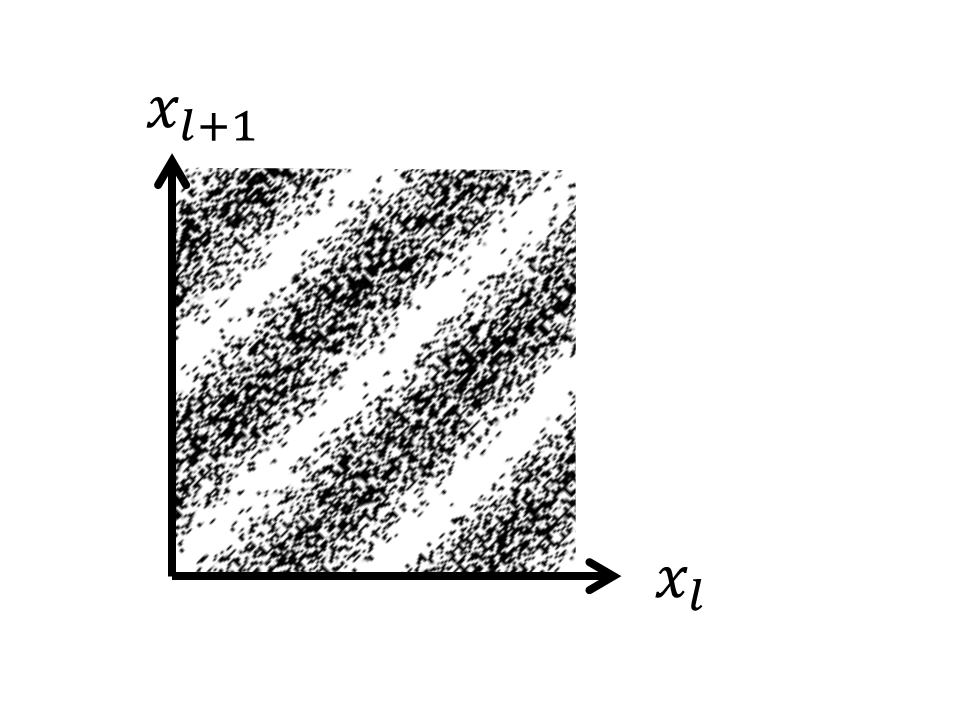
\includegraphics[width=\textwidth]{Folie13.png}
		\caption{Musterbildung als beispiel für schlechten Zufallszahlgenerator} 
		\label{fig:Interferenz}
		\centering
	\end{subfigure}
	~
	\begin{subfigure}[h]{0.5\textwidth}
		\centering
		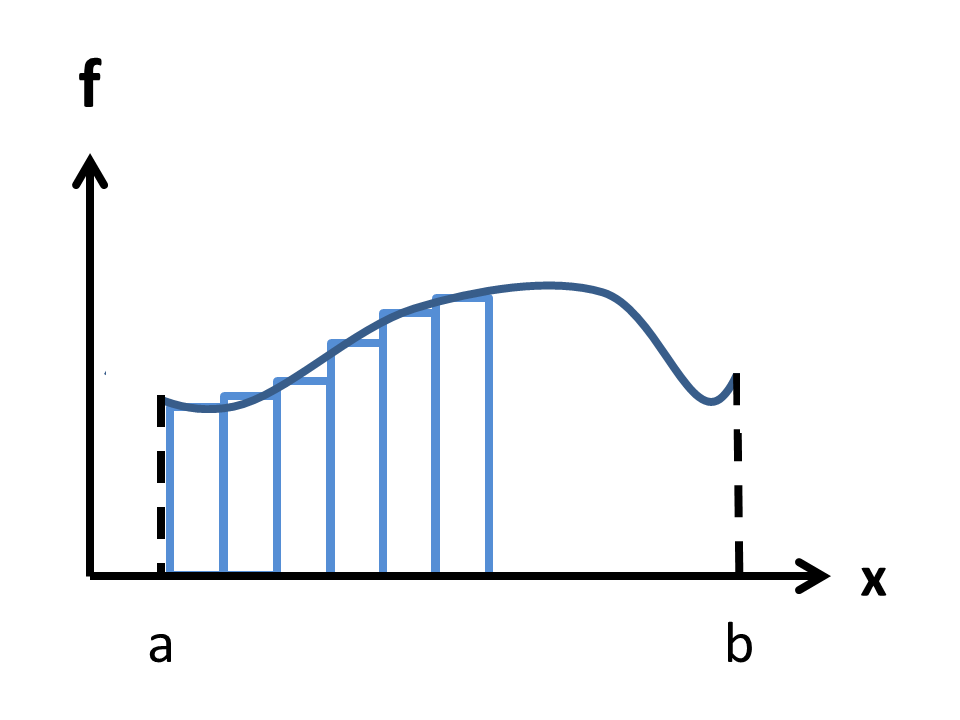
\includegraphics[width=\textwidth]{Folie14.png}
		\caption{Integral} 
		\label{fig:Integral}
		\centering
	\end{subfigure}
	\caption{ }
\end{figure}


\textbf{Beispiel:} $d=2 \; \to$ Abbildung \ref{fig:Interferenz}

Muster $\widehat{=}$ schlechter Zufallszahlengenerator. 

\item Momente testen: \\
Bilde \begin{align}
\frac{1}{N} \sum_{i=1}^N x_i^n
\end{align}
Falls zufällig verteilte $x_i$ (also gleichverteilt) gilt analytisch: \begin{align}
\overline{x_i^n} = \int _0 ^1 dx \; x_i^n = \frac{1}{n+1}
\end{align}
Dies muss auch stimmen für eine große Zahl $N$ von Zufallszahlen:
\begin{align}
\frac{1}{N} \sum_{i=1}^N x_i^n = \frac{1}{n+1}
\end{align}
\begin{itemize}
\item Es existieren zahlreiche Weiterentwicklungen des linear-konvergenten Zufallszahlen-Generators. (siehe z.B. \texttt{ rand()}), immer in C implementiert aber mit verschiedenen Methoden realisiert. 
\item bessere Zufallszahlen-Generatoren sind:
\begin{itemize}
\item Schieberegister (shift, Tanswert...TODO) Generator: Speichert Array von Zufallszahlen und berechnet die nächste Zufallszahl auf Basis mehrerer Vorgänger, \textbf{z.B} Kirchpatrick-Stall %TODO
$z[250]$ \begin{itemize}
\item $Z= Z[0] \underbrace{ \string^ }_\text{ \texttt{XOR} linewise} Z[147]$
\item dann wird Feld umsortiert
\item 250 Startwerte mit anderem Zufallszahlen-Generator %TODO 
\end{itemize}
\end{itemize}
\item seed reproduzierbar halten (wegen Reproduzierbarkeit wirtschaftlicher Ereignisse)
\item Programmbibliotheken!
\item Häufig sind anderen Verteilungsfunktionen gewünscht $\Rightarrow $ Transformationen
\end{itemize}

\end{enumerate}


\subsection{ Monte Carlo Integration}
Betrachten Integral (Abb. \ref{fig:Integral})
\begin{align}
I= \int_a^b f(x) \; dx
\end{align}
Konventionelle nummerische Methode: \\
Zerlegung in kleine Intervalle $\Delta x$:

\begin{align}
I_n= \sum_{\nu =1}^n \; \Delta x \; f(x_\nu) \quad \mbox{ \textbf{'Rechteckregel'}}
\end{align}
für $n \to \infty \Rightarrow I_N \to I$ (falls integrierbar).

Besser ist die Trapezregel oder die von Simpson. Sie sind im Prinzip 'gleich', unterscheiden sich allerdings bezüglich ihrer Konvergenz. \\

Verallgemeinerung auf höhere Dimensionen:

d-dimensionales Integral, $n$ Unterteilungen (Stützstellen) pro Achse \\
$\Rightarrow n^d$ Hypercubi der Göße $(\Delta x)^d$ und damit \\
$\Rightarrow n^d$ Terme müssen summiert werden\\
Für kleine $d$ kein Problem, für große jedoch absolut unmöglich. \\

\textbf{Beispiel:} (Phasenraumintegral) \\
 3TL, Freiheitsgrade $\mathbf{r}, \mathbf{p} \; \quad \Rightarrow$ Integral im Phasenraum: 

\begin{align*}
\int d^3 \mathbf{r}_1 d^3 \mathbf{r}_2 d^3 \mathbf{r}_3 \; d^3 \mathbf{p}_1 d^3 \mathbf{p}_2 d^3 \mathbf{p}_3 .... 
\end{align*} %TODO bild
ist immerhin 18-dimensional mit 
\begin{align*}
 n=100, d=18 \Rightarrow n^d=100^{18}=10^{36} \mbox{ Summanden (Rechenoperationen)}
\end{align*} 
Unsere Cluster schaffen $10^{10}$FLOPS
$\Rightarrow$ Summation dauert $10^{36 } / 10^{10}= 10^{26}s$ \\ (Vergleich: alter des Universums ist $10^{19}s$!) \\
Wir brauchen also ganz andere Methoden für hochdimensionale Integrale - die Statistik! 

Dafür betrachten wir wieder (der Einfachheit halber) folgendes Integral:
\begin{align}
I= \int_a^b f(x) \; dx
\end{align}

\begin{figure}[h] 
		\begin{subfigure}[h]{0.5 \textwidth}
		\centering
		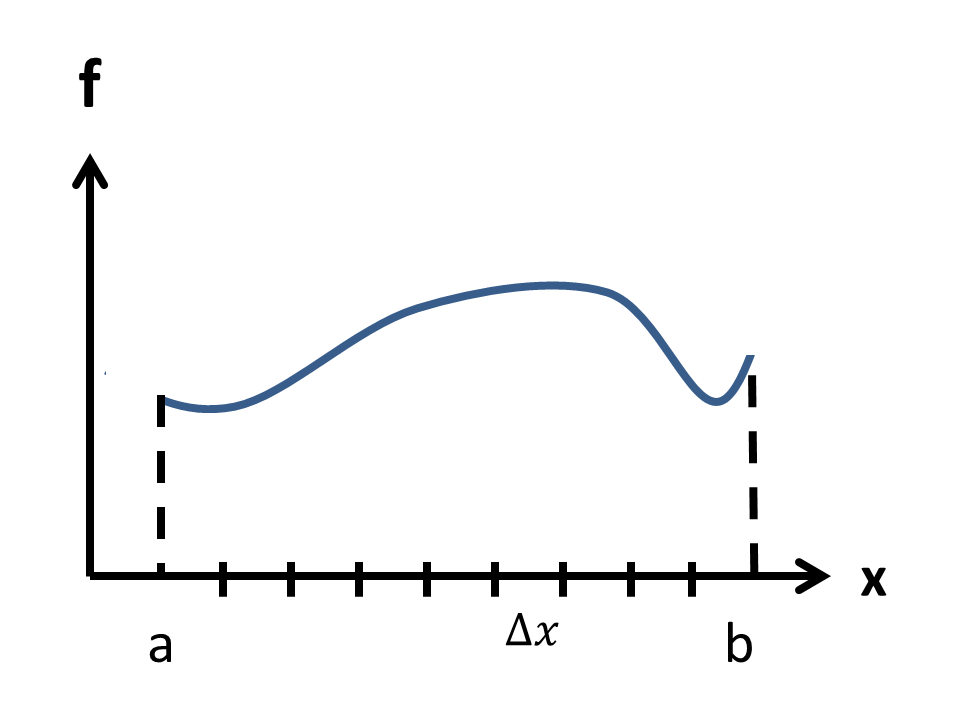
\includegraphics[width=\textwidth]{Folie15.png}
		\caption{Integral in Intervallzerlegung} 
		\label{fig:Intervall}
		\centering
	\end{subfigure}
	~
	\begin{subfigure}[h]{0.5\textwidth}
		\centering
		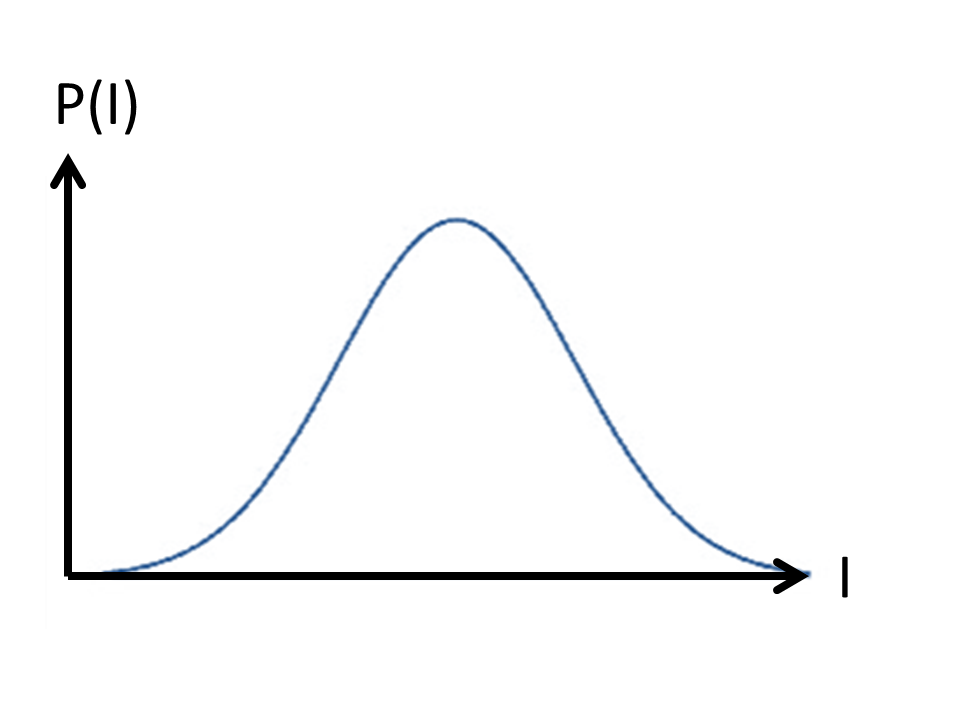
\includegraphics[width=\textwidth]{Folie16.png}
		\caption{Integral} 
		\label{fig:Integralwert}
		\centering
	\end{subfigure}
	\caption{ }
\end{figure}


mit $x_1,....x_N$ als $N$ gleichverteilte Zufallszahlen über $[a,b]$. 
Wir zerlegen das Intervall in $n$ Kästchen der Länge $\Delta x$, gemäß Abbildung \ref{fig:Intervall}.
$N_\mu$ sei weiterhin die Anzahl der $x_i$ im $\nu$ten Teilintervall. Dann gilt
\begin{align}
n \cdot \Delta x =&\;  b-a \; \quad
\Rightarrow \frac{\overline{N}_\nu}{N}= \frac{1}{n}= \frac{\Delta x}{b-a} \\
 \Rightarrow I= & \int_a^b f(x) \; dx  \approx  \sum_{\nu =1}^N \Delta x \; f(x_\nu )  \quad \quad \mbox{(Rechteckregel)} \\
 =& \sum_{\nu =1}^n (b-a)  \frac{\overline{N}_\nu}{N} f(x_\nu) 
= \frac{b-a}{N} \sum_{\nu =1}^n \underbrace{\overline{N}_\nu f(x_\nu)}_{ \approx \sum_{x_j \in [\,]_\nu} f(x_j)} \\ =& \frac{b-a}{N} \sum_{i=1}^N f(x_i)
\end{align}
Diese Formel ist nicht auf $d=1$ beschränkt, sondern gilt auch in höheren Dimensionen:
\begin{tcolorbox}[ams gather,title= , colback=blue!10!white, colframe=blue!30!black] 
 I \approx \frac{V_d}{N} \sum_{i=1}^N f(\mathbf{x}_i) 
\end{tcolorbox}
d.h. das Integral ist der Mittelwert der Funktionswerte an zufälligen Stützstellen $\mathbf{x}_i$.\\
\paragraph{Fehler:} (für $I = \int_0^1 f(x) dx$)\\
$\{ x_1, x_2,..., x_N\}$ sei spezielle Folge von Zufallszahlen mit $I_1$ als Integralwert (also Resultat). Eine andere Folge erzeugt anderes Ergebnis $I_2,...$. \\
$\Rightarrow$ Es existiert eine Wahrscheinlichkeitsverteilung $P(I)$ um dafür einen bestimmten Integralwert $I$ zu erhalten.  (Abb. \ref{fig:Integralwert})
Betrachte deswegen unendliche viele Ketten\footnote{$\to$ exaktes Resultat, aber wie groß ist dann die Schwankung?} von Zufallszahlen der Länge $N$:\\
$\Rightarrow P(I) dI$ wäre dann die Wahrscheinlichkeit, dass $I$ im $I$-ten Intervall $dI$ um $I$ liegt.
\begin{align}
\langle I \rangle =& \int dI \; P(I) \; I \; \quad \quad \left( \mbox{ mit } I= \frac{1}{N} \sum_{i=1}^N f(x_i)= I(x_1,x_2,...,x_N) \right) \\
=& \int dx_1,...,dx_N \; \rho(x_1) ... \rho(x_N) \; \frac{1}{N} \sum_{i=1}^N f(x_i) \\
=& \int_0^1 dx \; f(x) 
\end{align}
unendlich viele Folgen von Zufallszahlen der Länge $N$ liefern gemittelt das exakte Ergebnis! Die Berechnung des Fehlers folgt dann:
\begin{align}
\langle (I- \langle I \rangle)^2 \rangle =& \langle I^2 \rangle - \langle I \rangle ^2 \\
=& \langle \frac{1}{N^2} \left( \sum_{i=1}^N \; f(x_i) \right) ^2 \rangle - \langle \frac{1}{N} \sum_{i=1}^N \; f(x_i)\rangle^2 \\
=& \frac{1}{N^2} \sum_{i,j=1}^N \langle f(x_i) \; f(x_j) \rangle - \frac{1}{N^2} \sum_{i,j=1}^N \langle f(x_i) \rangle \; \langle f(x_j) \rangle \\
=& \frac{1}{N^2} \sum_{i=1}^N \langle f(x_i)^2 \rangle - \frac{1}{N^2} \sum_{i=1}^N \langle f(x_i) \rangle ^2 \; +\mathcal{O} \quad \mbox{ für } i = j
\end{align}

weil
\begin{align*}
\langle f(x_i) \; f(x_j) \rangle = \langle f(x_i) \rangle \; \langle f(x_j) \rangle \; \mbox{ für } i \neq j
\end{align*}

brauche
\begin{align}
\int dx_1 dx_2 \; & \rho(x_1) \rho(x_2) \; f(x_1) f(x_2) \\
&= \int dx_1 \rho(x_1)f(x_1)  \underbrace{\int dx_2 \rho(x_2)}_\text{=1}\times  \int dx_2 \rho(x_2)f(x_2) \cdot \underbrace{\int dx_1 \rho(x_1)}_\text{=1} 
\end{align} 
aber
\begin{align*}
\int dx_1 \; \rho (x_1) f(x_1)^2 \neq \left( \int dx_1 \; \rho (x_1) f(x_1) \right) ^2
\end{align*}

\begin{align*}
 \Rightarrow \langle \Delta I \rangle ^2= \frac{1}{N} \left( \langle f(x)^2 \rangle - \langle f(x) \rangle^2 \right)
\end{align*}
\paragraph{Diskussion:} \begin{itemize}
\item[1)] Konvergenz:
\begin{align}
\Delta I \propto \frac{1}{\sqrt{N}}
\end{align}
Zum Vergleich der Konvergenz mit herkömmlichen Methoden, \textbf{z.B.} der Trapezregel. Ihr Fehler in einer Dimension ist $\propto h^2 $. $N$ Rechenschritte: $h \propto N^{ \frac{-1}{d} }$ in $d$ Dimensionen. $\Rightarrow \Delta I \propto N^{\frac{-2}{d}}$\\
$ \Rightarrow$ für $d<4$ ist Monte Carlo 'besser' als Trapezregel

\item[2)] $I \to \langle I \rangle$ für $N \to \infty$. \textit{Eine} $\infty$-lange Kette (o. Folge) führt (auch) zum exakten Resultat, d.h. das Verfahren ist sebstmittelnd.

\begin{figure}[h] 
		\begin{subfigure}[h]{0.5 \textwidth}
		\centering
		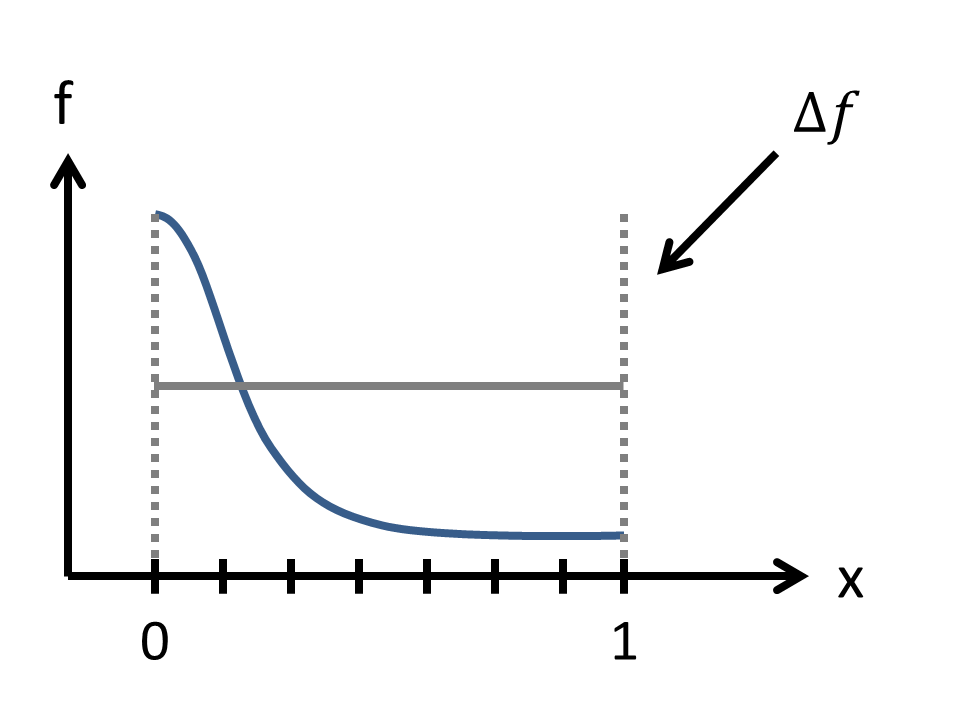
\includegraphics[width=\textwidth]{Folie17.png}
		\caption{Dichtefluktuation} 
		\label{fig:Dichtefluktuation}
		\centering
	\end{subfigure}
	~
	\begin{subfigure}[h]{0.5\textwidth}
		\centering
		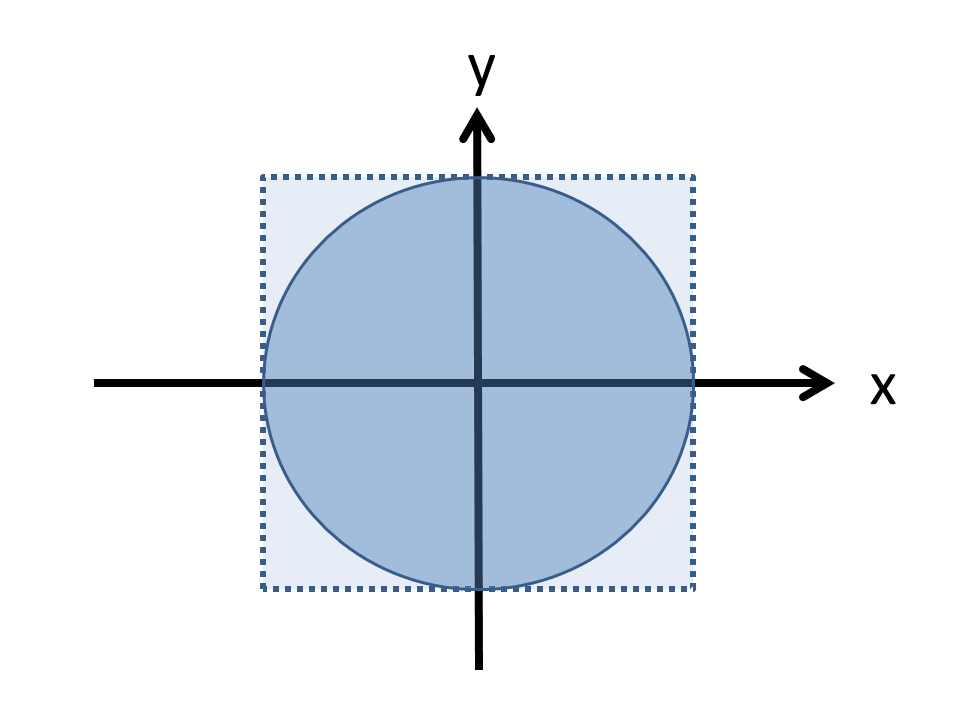
\includegraphics[width=\textwidth]{Folie18.png}
		\caption{Volumen einer $2-$dimensionalen Kugel}
		\label{fig:Kugel}
		\centering
	\end{subfigure}
	\caption{ }
\end{figure}



\item[3)] Verfahren gut, wenn $f$ möglichst konstant.  Anschaulich in Abbildung . Man sieht (Abb. \ref{fig:Dichtefluktuation}), dass das Verfahren exakt ist, falls $f= const.$
\item[4)]Der Fehler lässt sich während der Integration berechnen und sollte endlich bleiben.
\end{itemize}
\textbf{Beispiel:} (Volumen einer D-Dimensionalen Einheitskugel) \\
Wir starten in 2D, gemäß Abbildung \ref{fig:Kugel}.
\begin{align*}
f(x,y)=
\begin{cases}
1 & x^2+y^2 <1 \\
0 & \mbox{sonst}
\end{cases}
\end{align*}
Flächenberechnung: 
\begin{align*}
I= \int_0 dx \; dy \; 1 = \int_{-1}^1 dx \int_{-1}^1 dy \; f(x,y) 
\approx \frac{4}{N} \sum_{i=1}^N f(x_i,y_i)
\end{align*}
mit $[x_i, y_i]$ gleichverteilt aus $[-1,1]$.

\begin{figure}[h] 
		\begin{subfigure}[h]{0.5 \textwidth}
		\centering
		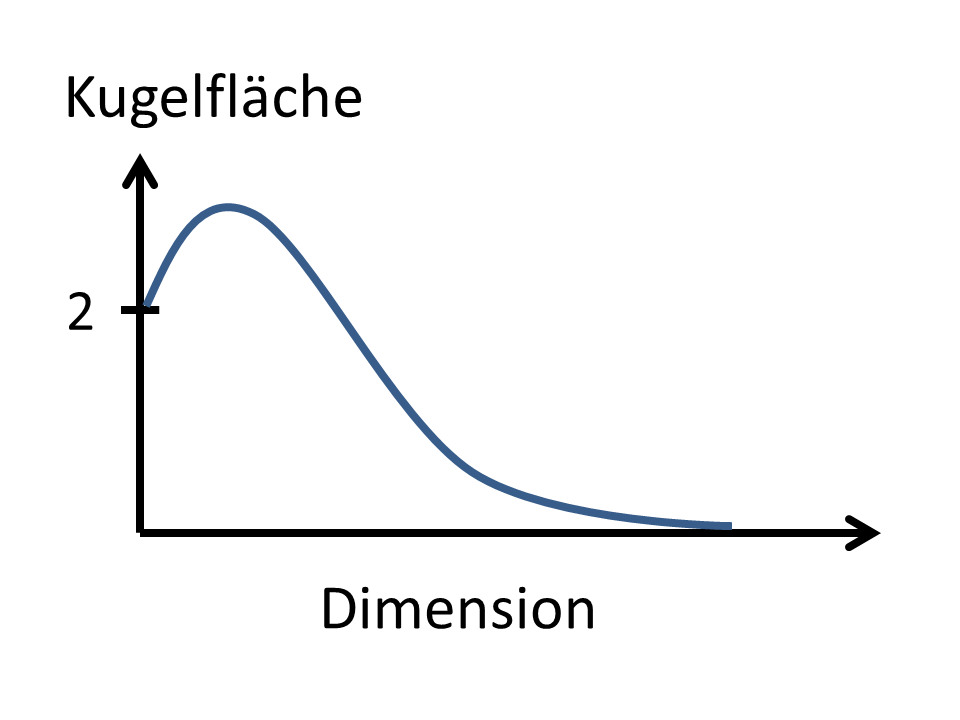
\includegraphics[width=\textwidth]{Folie19.png}
		\caption{Relatives Volumen für wachsende Dimension} 
		\label{fig:RelativesVolumen}
		\centering
	\end{subfigure}
	~
\begin{subfigure}[h]{0.5\textwidth}
		\centering
		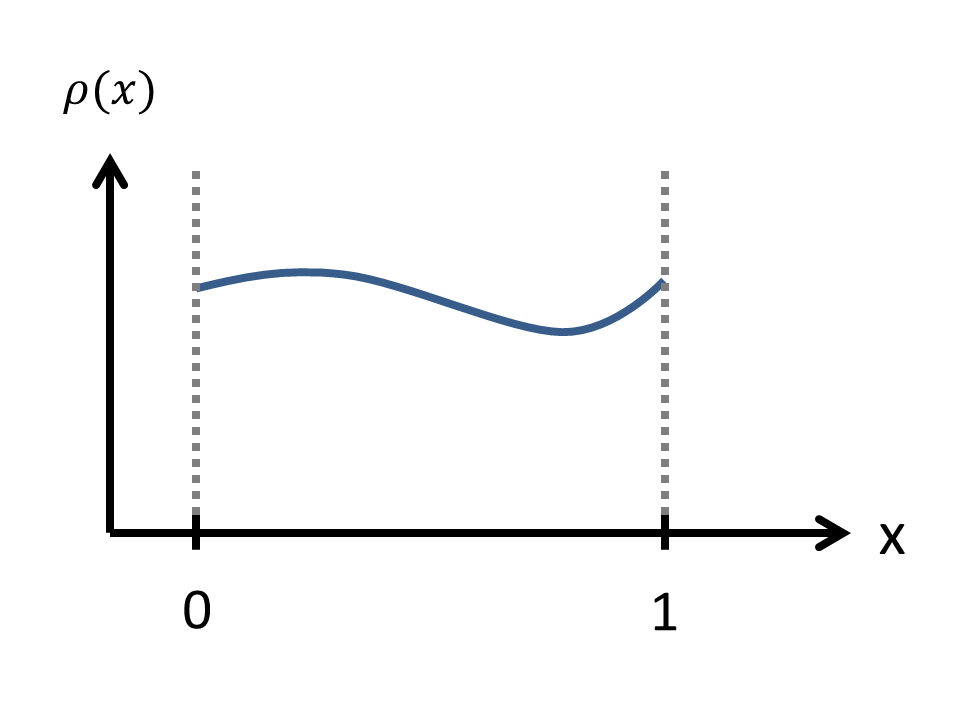
\includegraphics[width=\textwidth]{Folie22.png}
		\caption{Problemstellung}
		\label{fig:Problemstellung}
		\centering
	\end{subfigure}
	\caption{ }
\end{figure}	
	

\begin{figure}[h] 
		\begin{subfigure}[h]{0.5 \textwidth}
		\centering
		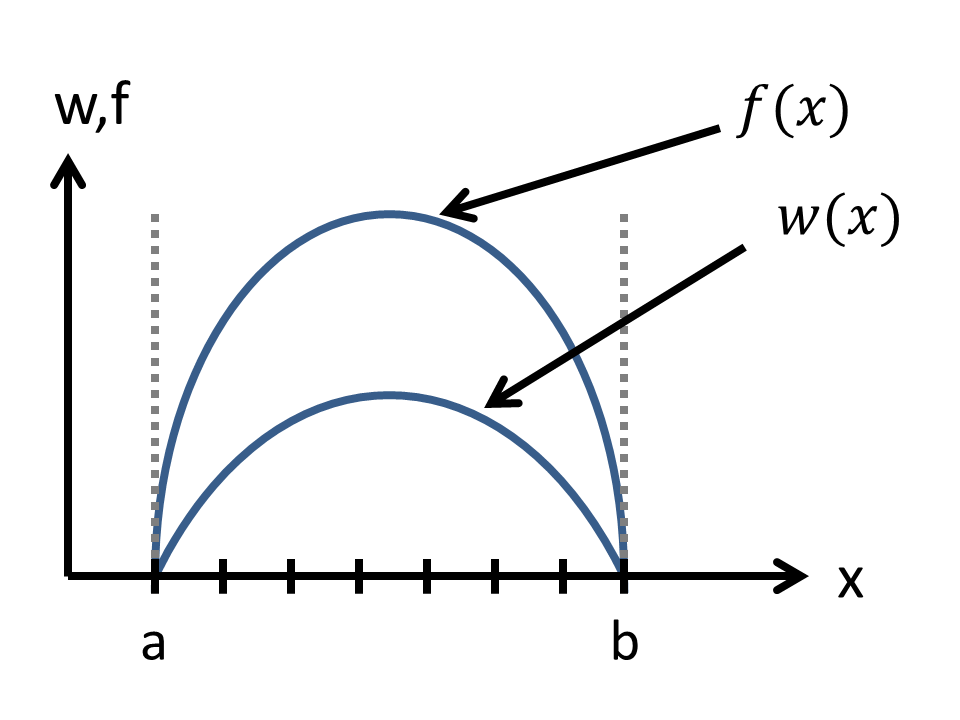
\includegraphics[width=\textwidth]{Folie20.png}
		\caption{} 
		\centering
	\end{subfigure}
	~
\begin{subfigure}[h]{0.5\textwidth}
		\centering
		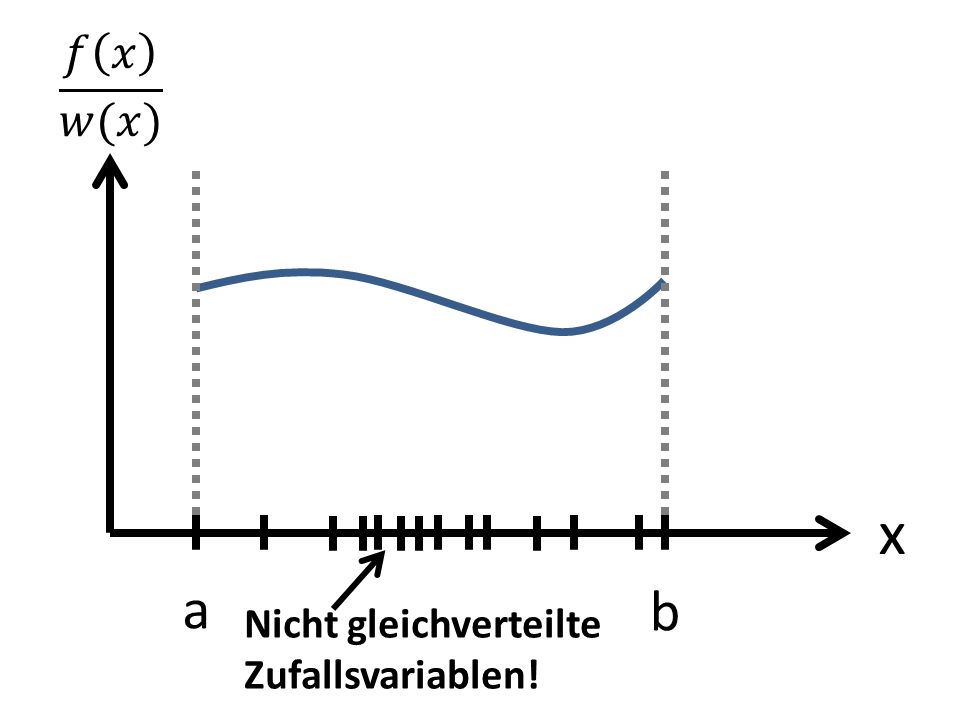
\includegraphics[width=\textwidth]{Folie21.png}
		\caption{}
		\centering
	\end{subfigure}
	\caption{ Importance sampling}
	\label{fig:Funktion}
\end{figure}
	
 


Zeige Programm: Das Volumen verschwindet für hohe Dimensionen: Eindimensionale Betrachtung: Intervall geht exakt von $[-1,1]$, bei einem Kreis in $[-1,1] \times [-1,1]$ fallen schon die Ecken weg. Das Volumen auf den Einheitsradius ist nicht mehr ganz so groß. Bei drei Dimensionen fallen schon die 8 Ecken weg, daher nimmt das relatives Volumen für große Dimensionen ab. (Abbildung \ref{fig:RelativesVolumen}) \\
$\to$ Wie kann man das Verfahren verbessern?

\paragraph{Verbesserung:}
\begin{align}
(\Delta I )^2 = \frac{1}{N} \underbrace{\left( \langle f^2(x) \rangle - \langle f(x)\rangle^2 \right)}_\text{Schwankungsbreite der Fkt}
\end{align}
Idee: Transformation, so dass der Integrand $\approx const$, dafür aber Zufallszahl \textit{nicht} gleichverteilt.
\begin{tcolorbox}[ams gather,title= , colback=blue!10!white, colframe=blue!30!black] I= \frac{1}{N} \sum_{i=1}^N \frac{f(y_i)}{w(y_i)} 
\end{tcolorbox}

wobei $y_i$ eine Folge von Zufallszahlen gemäß Verteilung $w(y)$ mit $w(y)>0$, $\int w(y) \; dy=1$. \\
Beweis:
\begin{align}
\langle I\rangle = \langle \frac{1}{N} \sum_{i=1}^N \frac{f(y_i)}{w(y_i)} \rangle = \frac{1}{N} \sum_{i=1}^N \langle \frac{f(y_i)}{w(y_i)} \rangle = \frac{1}{N} \sum_{i=1}^N \int dy_i \; w(y_i)  \frac{f(y_i)}{w(y_i)} 
= \int dx \; f(x)
\end{align}
Fehler: \begin{align}
\Delta I=\frac{1}{\sqrt{N}}
 \sqrt{\langle \left(\frac{f}{w}\right)^2 \rangle - \langle \frac{f}{w} \rangle ^2}
 \end{align}
 
 

 
 
 $\Rightarrow$ für kleine Felder: $w$ so wählen, dass $\frac{f}{w} \approx const.$ Man muss allerdings $w$ integrieren können und $w$ muss $f$ ähnlich sein und man braucht Zufallszahlen mit einer vorgegebenen Verteilung! (Abbildung \ref{fig:Funktion})
 
 
 $\Rightarrow$ Mann nennt dieses Verfahren:\textbf{Importance sampling}, (weil 'wichtige'$\widehat{=}$ 'hohe' Werte des Integranden $f(x)$ in der ursprünglichen Funktion häufiger genommen werden, im Gegensatz zum herkömmlichen \textbf{simple sampling})\\ $\Rightarrow$ die Wurzel N im Fehler ist geblieben. Leider konnten wir die Konvergenz dadurch nicht verstärken. Neues Problem hierbei ist jetzt: 
 
 \subsection{Zufallszahlen einer vorgegebenen Verteilung}
 

 
 Problem: (Problemstellung siehe Abbildung \ref{fig:Problemstellung}).
 Zufallszahlen $x_i$ aus einem Intervall berechnen mit einer Verteilung $\rho(x)$ mit
 \begin{itemize}
 \item $\rho(x)>0$
 \item $\int_0^1 dy \rho(x)=1$.
\end{itemize} 
 

 
 \begin{figure}[h] 
		\begin{subfigure}[h]{0.5 \textwidth}
		\centering
		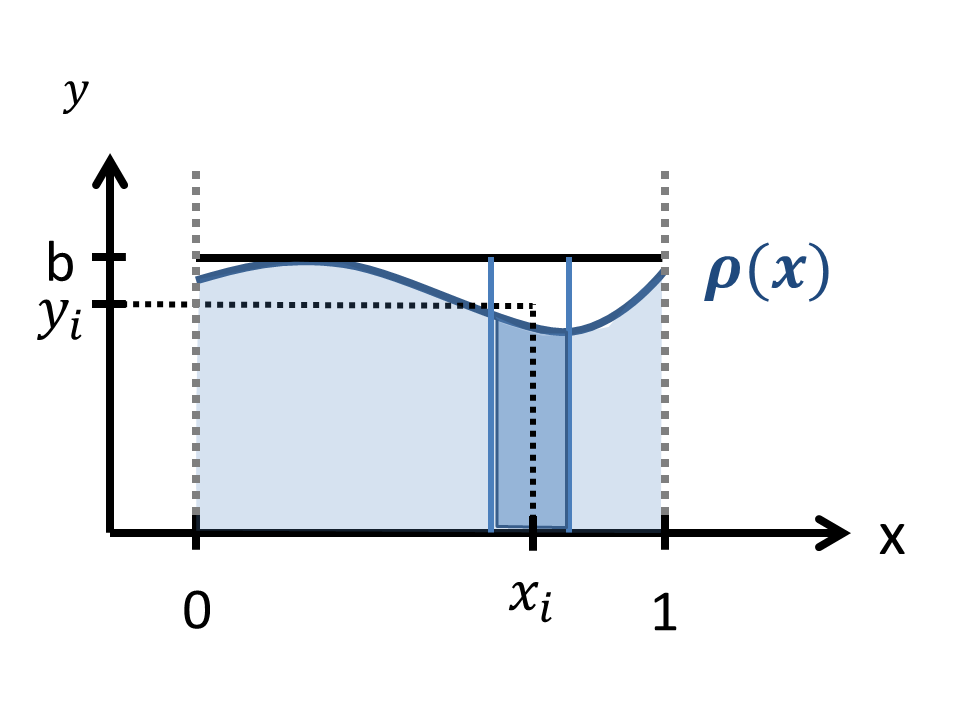
\includegraphics[width=\textwidth]{Folie23.png}
		\caption{Rejection Method} 
		\label{fig:Neumann}
		\centering
	\end{subfigure}
	~
\begin{subfigure}[h]{0.5\textwidth}
		\centering
		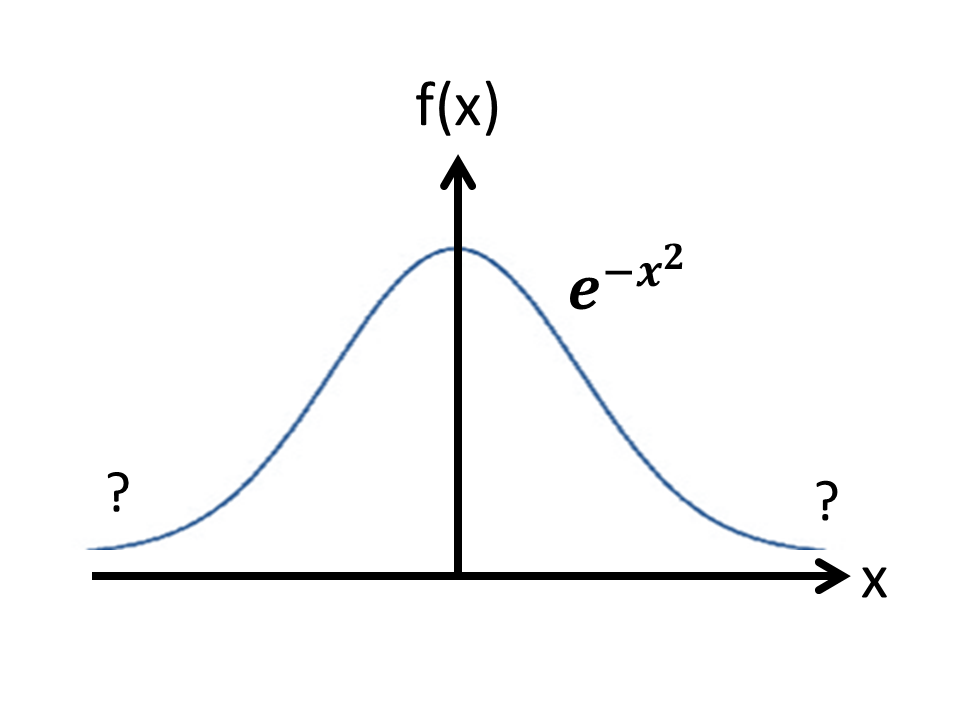
\includegraphics[width=\textwidth]{Folie24.png}
		\caption{\textsc{Gauß}-Funktion}
		\label{fig:Gaussunktion}
		\centering
	\end{subfigure}
	\caption{ }
\end{figure}	

 \begin{itemize}
 \item[a)] \textbf{Rejection-Method} nach \textsc{von Neumann} (1947) \\ (Abbildung \ref{fig:Neumann}).
 betrachte Paar von Zufallszahlen, $x_i \in [0,1], y_i \in [0,b]$ mit $b=Max(\rho(x))$.
 
$\to$ wenn $y_i < \rho(x_i) \Rightarrow x_i$ wird akzeptiert mit $\xi_i=x_i$\\
 $\to$ wenn $y_i > \rho(x_i) \Rightarrow x_i$ wird nicht akzeptiert. \\
 
 $\Rightarrow$ Folge von Zufallszahlen $\xi_i$. Zahl der $\xi_i \in \Delta x$ ist proportional zur Fläche $\rho(x) \cdot \Delta x$ und damit proportional zu $\rho(x)$.
 
 \textbf{Problem:} viele Züge notwendig, wenn selten akzeptiert wird. 
 
 \textit{Schlecht wäre zum Beispiel:} die Betrags-Exponentialfunktion (\textsc{Gauß}funktion) benötigt ein großes $x-$Intervall: Abbildung \ref{fig:Gaussunktion}.
 
\textit{Gut wäre dafür aber:} Kugeln - 
Vektoren innerhalb (oder auf) Einheitskreis



\item[b)] \textbf{Transformationsmethode} \\
betrachte monotone Funktion (Abbildung \ref{fig:Problemstellung}) . Dabei seien wieder $x_i$ gleichverteilte Zufallsvariablen aus $x_i \in [0,1]$ und $y_i = f(x_i)$.Frage: Wie sind die verteilt? \footnote{Dafür muss man die Wahrscheinlichkeiten umrechnen. In ein $\Delta x$ fallen irgendwelche Zufallsvariablen rein und werden auf $\Delta y$ abgebildet, das ja kleiner sein kann. Die dichte in $\Delta y$ sowie $\Delta x$ kann also verschieden sein.} %TODO siehe image

$N$ Zufallszahlen \\
 $\Rightarrow$ $N \cdot \Delta x$ fallen in das Intervall $\Delta x$. Die entsprechenden abgebildeten Zufallszahlen $y_i=f(x_i)$ fallen in $\Delta y$ um $f(x)$.

$\Rightarrow$ Änderung der Punktdichte $\rho(y)\Delta y = \Delta x$. \\
Der limes $\Delta x \to 0$ mit 
\begin{align*}
\rho(y)=\frac{dx}{dy}
\end{align*}
soll vorgegeben werden. Wie lautet dann $f(x)$?
\begin{align}
\Rightarrow  \int_0^x dx' = \int \rho(y) dy \; \Rightarrow \; x(y) = \int \rho(y) \; dy = x(y) = f^{-1}(y) 
\end{align}
\begin{tcolorbox}[ams gather,title=, colback=blue!10!white, colframe=blue!30!black] 
 f(x)= \left( \int \rho(y) \; dy \right)^{-1} 
\end{tcolorbox}
\begin{align*}
\Rightarrow  f(x_i)=y_i \mbox{ sind gesuchte ZZ}
\end{align*} 
also: $\rho(y)$ gegebene Verteilung muss man 
\begin{enumerate}
\item[1)] Integrieren
\item[2)] Invertieren
\end{enumerate}

\textbf{ Beispiel:}
 \begin{align*}
  \rho(y)=
 \begin{cases}
e^{-y} & \text{für } y \geq 0 \\
0 & \text{für } y < 0.
 \end{cases}
 \end{align*}
 und wie gewünscht 
 
 \begin{itemize}
	 \item Normierung 
  		$\int_0^\infty  \rho(y) \; dy = 1 $
 	\item Positiv
 		$\rho(y) \geq 0 $
\end{itemize}

 \begin{enumerate}
 \item Es gilt: \begin{align*}
 \int_0^y dy' \rho(y') = 1- e^{-y} \equiv x(y)
 \end{align*}
 \item Umkehrfunktion:
  \begin{align*}
 y= - ln(1-x) = f(x)
 \end{align*}
 $\Rightarrow$ ziehe gleichverteilte Zufallszahl $x_i \in [0,1)$ (nicht die 1 selber!) \\
 $\Rightarrow y_i = -ln(1-x_i)$ sin exponentiell verteilte Zufallszahlen $\in [0,\infty]$.
 \end{enumerate}
 Nachteil: 
\footnote{Der Computer ist nicht so schnell beim logarithmieren...deswegen ist die rejection Methode diesbezüglich interessanter.}
Man muss die gewünschte Verteilung $\rho(y)$ erst integrieren und dann zusätzlich auch invertieren können. Dies geht nicht bei \textbf{z.B.} der \textsc{Gauß}-Verteilung

\item[c)] \textbf{Gauß-Verteilung } (Normalverteilung) \\
\begin{align*}
\rho(x)= \frac{1}{\sqrt{2 \pi} \sigma} e^{-\frac{x^2}{2 \sigma^2}}
\end{align*}
Wieder gilt:
 \begin{itemize}
	 \item Normierung 
  		$\int_0^\infty  \rho(y) \; dy = 1 $
 	\item Positiv
 		$\rho(y) > 0 $
\end{itemize}


Sie ist nicht analytisch (bestimmt) integrierbar, sodass die Transformationsmethode nicht anwendbar ist. Dafür gibt es aber einen Trick: \\

\begin{figure}[h] 
		\begin{subfigure}[h]{0.5 \textwidth}
		\centering
		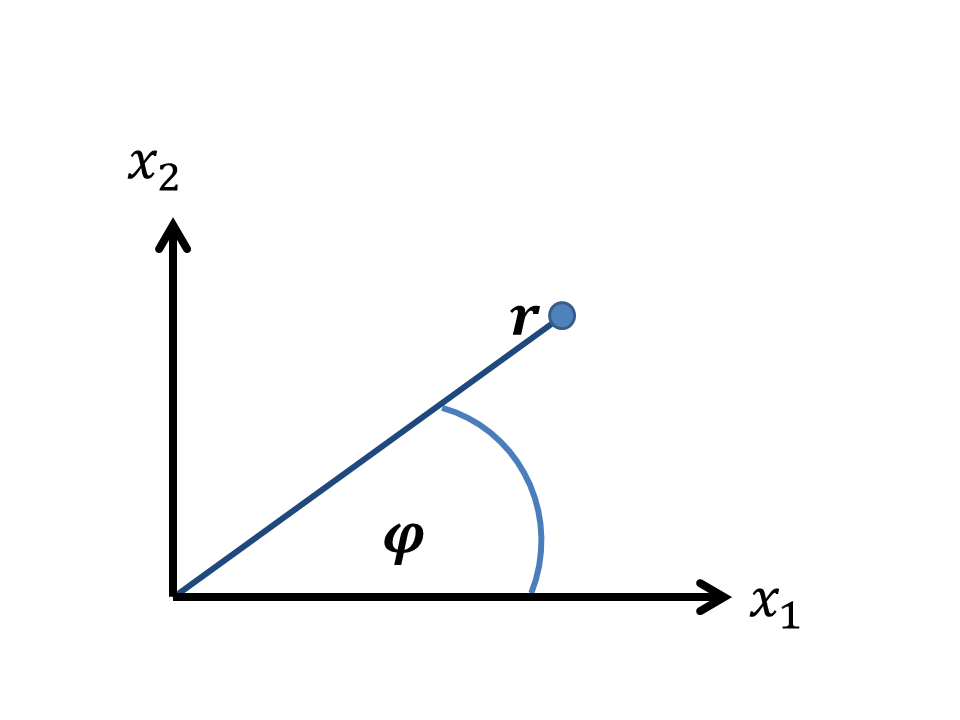
\includegraphics[width=\textwidth]{Folie25.png}
		\caption{Kugelkoordinaten} 
		\label{fig:Kugelkoordinaten}
		\centering
	\end{subfigure}
	~
\begin{subfigure}[h]{0.5\textwidth}
		\centering
		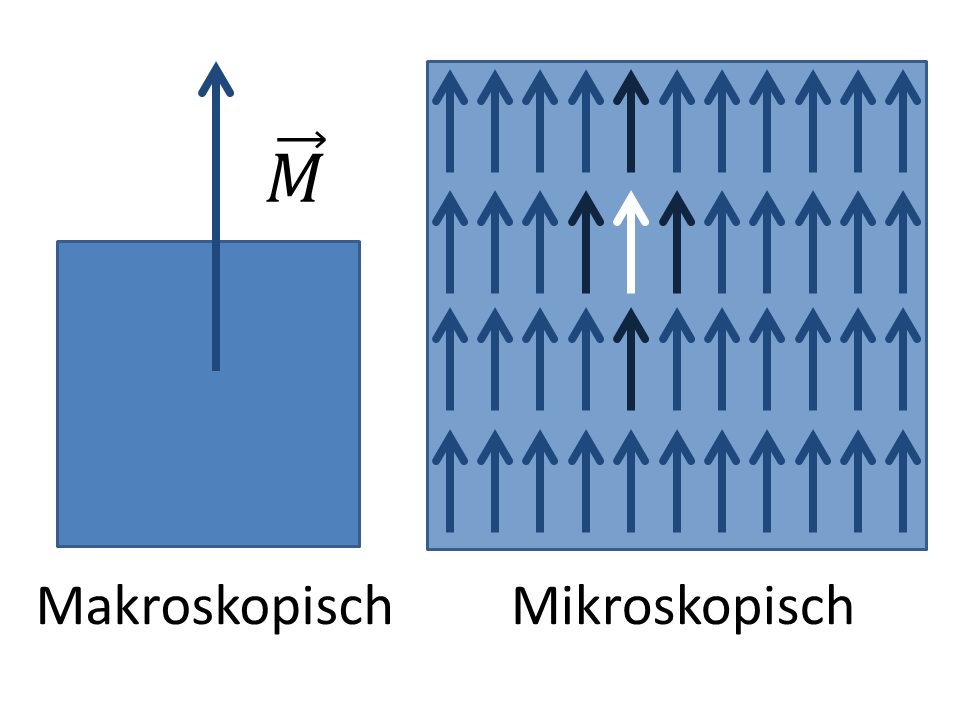
\includegraphics[width=\textwidth]{Folie26.png}
		\caption{Modell des Ferromagneten}
		\label{fig:Ferromagnet}
		\centering
	\end{subfigure}
	\caption{ }
\end{figure}	


betrachte eine zweidimensionale Wahrscheinlichkeitsverteilung
\begin{align}
p(x_1,x_2)=\frac{1}{	2 \pi \sigma^2} e^{- \frac{x_1^2 + x_2^2}{2 \sigma^2}} = \rho(x_1) \cdot \rho(x_2)
\end{align}
die Zahl der Punkte im Intervall $dx_1, dx_2$ ist:
\begin{align}
\frac{1}{	2 \pi \sigma^2} e^{- \frac{x_1^2 + x_2^2}{2 \sigma^2}} dx_1 dx_2= & \frac{1}{	2 \pi \sigma^2} e^{- \frac{r^2}{2 \sigma^2}} \;r \; dr  d\phi \quad \left( \mbox{subst: } u = \frac{r^2}{2 \sigma^2} \right) \\
= & \frac{1}{2 \pi} e^{-u} du \; d\phi
\end{align}
mit Koordinaten (Abb. \ref{fig:Kugelkoordinaten})
\begin{align*}
x_1=  r cos(\phi) = \sigma \sqrt{2 u} \; cos(\phi) \\
x_2=  r sin(\phi)= \sigma \sqrt{2 u} \; sin(\phi)
\end{align*}
also...
\begin{itemize}
\item[...] ziehe: 
\begin{itemize}
\item[-] Zufallszahl $\phi_i$ aus $[0,2\pi]$
\item[-] Zufallszahl $y_i$ ist exp-verteilt aus $[0, \infty]$
\end{itemize}
\item[...]rechne:
\begin{itemize}
\item[-] $x_i = \sigma \sqrt{2 u_i} \; cos(\phi)$
\item[-] $x_i' = \sigma \sqrt{2 u_i} \; sin(\phi)$
\end{itemize}
\end{itemize}



praktisch:
\begin{tcolorbox}[ams gather,title=, colback=blue!10!white, colframe=blue!30!black] 
x_{2i}= \sigma \sqrt{-2 ln(1-y_{2i})} \; cos(2\pi \; y_{2i-1}) \\
\mbox{ mit } \quad y_i\mbox{ ZZ} \in [0, 1) \mbox{ gleichverteilt} \nonumber
\end{tcolorbox}
Beispiel: Wir nehmen das Integral
\begin{align*}
\int_0^{2\pi} x \; e^x \; dx \underbrace{=}_\text{analytisch} e^{2\pi} (2\pi -1) +1
\end{align*} 
Importance: \begin{align*}
\rho(y)= \frac{e^y}{e^{2\pi} -1}\quad  \left( \mbox{normiert } \int_0^{2\pi} e^y \; dy =1 \right) 
\end{align*}
\begin{align*}
\int_0^y \rho(y') \; dy' = \frac{e^y - 1}{e^{2\pi} - 1} = x(y)
\end{align*}
\begin{align*}
 \Rightarrow y= ln(\underbrace{(e^{2\pi}-1)}_\text{Norm.-Konst} x+1) 
 \end{align*}
 \begin{align*}
\Rightarrow  I = \frac{1}{N} \sum_{i=1}^N \frac{f(y_i)}{\rho(y_i)}= \frac{1}{N} \sum_{i=1}^N y_i (e^{2\pi}-1)
\end{align*}
wobei $x_i \in [0,1)$.
\end{itemize}

 
% %TODO Review:
% Importance sampling: \begin{equation}
% i= \frac{1}{N} \sum_{i=1}^N \frac{f(y_i)}{w(y_i)} \mbox{ mit } y_i: \mbox{ Zufallszahl normalverteilt }
% \end{equation}
% 
%\textbf{ Beispiel: }
% \begin{align}
% \int_0^{2\pi} x \; e^x \; dx = e^{2\pi} (2\pi -1) +1\\
% \rho (y)= \frac{e^y}{e^{2\pi}-1} \\
% y= ln \left( (e^{2\pi} -1)\; x \; +1\right) \mbox{ mit } x \in [ 0,1] \\ \Rightarrow I= \frac{1}{N}\sum_{i=1}^N y_i (e^{2\pi}-1)
% \end{align}
% %TODO Review END
 
 \subsection{Ising Modell}
 Das \textsc{Ising}Modell\footnote{Zweizustandsmodell: minimales Modell für ein reales system, jeder einzelne Freiheitsgrad hat nur zwei Zustände, ist aber das erste Modell das einen Phasenübergang zeigt. Es ist im $2d$ Fall aber exakt lösbar und daher gut für uns.} findet zahlreiche Anwendungen (\textbf{z.B.} in den Sozialwissenschaften, in der Physik für Fest-Flüssig-Übergänge oder mehr noch für \textit{magnetische Eigenschaften}, wie etwa dem Ferromagneten). Es ist \textit{sehr einfach} und zudem auch \textit{exakt lösbar} für Lösungen im $1d$ (\textsc{Ising}), $2d $ (\textsc{Onsager}) Fall.
($\to$ Nobelpreis) \\
Wir benutzen das Modell eines Ferromagneten, gemäß Abbildung \ref{fig:Ferromagnet}.  \\
Makroskopisch ist eine Gesamtmagnetisierung zu beobachten. Auf mikroskopischer Ebene findet man Atome mit 'Spin', atomare Momente, die in eine Richtung ausgerichtet sind. Sie wechselwirken mit ihren umliegenden Nachbarn\footnote{ Die Wechselwirkung ist im einfachsten Fall nur mit den nächsten Nachbarn, Idee: Überlapp der Wellenfunktion ist begrenzt exponentiell}. Es gibt Vorzugsrichtungen, abhängig von den Kristallstrukturen (Wegen Spin-Bahn Wechselwirkungen) \\
$\Rightarrow$ Vorzugsachse (\textbf{Anisotropie}). Der Kristall hat eine leichte Achse, d.h. Spins wollen in diese Richtung stehen.\\
$\Rightarrow$ nur noch zwei Zustände! ('rauf' $\uparrow$ oder 'runter' $\downarrow$) \\

 \begin{itemize}
\item[-] Gitter aus Spins, im einfachsten Fall $S= \pm 1$, sodass beispielsweise $S_i$ nur Index $i= \{+,-\}$ hat.
\item[-]Hamilton-Funktion\footnote{Spin ist hier kein Drehimpuls sondern wirklich ein Spin, das Minuszeichen kommt vom Drehimpuls des \textit{Elektrons}. Es ist ein phänomenologisches klassisches Modell, also nicht wirklich ein quantenmechanisches Spin-$1/2$-Modell sonder im klassischen Limes (Limes Heisenbergmodell und gleichzeitig Anisotropie gegen unendlich)}
\begin{align}
H= - \sum_{i=1}^N B \; S_i
\end{align}
\begin{itemize}
\item[-] $B> 0 : \; S_i = 1$ günstig 
\item[-]  $B<0 : \; S_i = -1$ günstig 
\item[-] $B=0; \; S_i = \pm 1$ unmöglich
\end{itemize}
 \item[-]Hinzüglich einer \textbf{Wechselwirkung:} Überlapp der Wellenfunktion führt zu Austauschenergie $J$ zwischen denjenigen Spins, die nächste Nachbarn sind. (Dies ist nicht die makroskopische (Dipol-)Wechselwirkung) 
 
 \begin{align}
  H(S_1, S_2, ..., S_N) = \underbrace{ -J \sum_{i,j=1;\; i,j NN}^N S_i S_j }_{\substack{\text{Nachbarn auf dem Gitter} \\ \text{jedes Paar einmal}}} - B \sum_{i=1}^N S_i
\end{align}  
($B$ gibt vor, welche Ausrichtung energetisch günstiger ist. Beispiel: $\uparrow \uparrow, B: \Uparrow$)
  \begin{itemize}
  \item $J>0: \; \uparrow \uparrow  \quad E= -J$ günstig $\rightarrow$ Ferromagnet
  \item $J<0: \; \uparrow \downarrow  \quad E= -J$ günstig $\rightarrow$ eventuell Antiferromagnet ($\uparrow \downarrow \; , \; \downarrow \uparrow$)
  \end{itemize}
  Im Folgen $J>0$. 

\begin{enumerate}
\item Grundzustand (Kette): $E_0= -J(N-1)-BN $. $\uparrow \uparrow \uparrow \uparrow \uparrow \uparrow$
\item Endliche Temperatur $T$: angeregte Zustände kommen vor, z.B. $\uparrow \uparrow \uparrow \downarrow \uparrow$ \textit{(erster angeregter Zustand)}
\end{enumerate}

\textbf{Beispiel:} System mit abzählbar vielen (quantisierten) Zuständen.  
\begin{align*}
N(4) \mbox{ Spins, } S= \frac{1}{2} \quad \quad \Aboxed{ \uparrow \downarrow \uparrow \uparrow }
\end{align*}
Wie berechnet man nun das \textbf{thermische Mittel} einer Observablen?
\begin{align}
\langle \Omega \rangle= \sum_{ \{\bar{S} \}}  p(\{ S \}) \; \Omega(\{S\})
\end{align}
Dabei ist $\{ S \}$ ein Zustand des Systems und $\Omega(\{ S \})$ die zu diesem Zustand gehörende Größe. Die Wahrscheinlichkeit $p(\{ S \})$ meint die Wahrscheinlichkeit, dass das System in diesem Zustand ist. Eine vereinfachte Schreibweise ist
\begin{align*}
\{ S \} \; \widehat{=} \; \underline{S}
\end{align*}
Wir nummerieren die Zustände durch
\begin{align}
\langle \Omega \rangle = \sum_{\underline{\dot{S}}} p_{\underline{\dot{S}}} \; \Omega_{\underline{\dot{S}}}
\end{align}
wobei man zeigen kann dass:

%\item[-] kanonische Gesamtheit 
\begin{align}
p_{\underline{\dot{S}}} = p ( H_{\underline{\dot{S}}}) = \frac{e^{- \beta H_{\underline{\dot{S}}} }}{\underbrace{ 
\sum_{\underline{\dot{S}}}  e^{-\beta H_{\underline{\dot{S}}} } 
}_{\text{Normierung:} \sum_{\underline{\dot{S}}} p_{\underline{\dot{S}}} =1 }}\; , \quad \beta = \frac{1}{k_BT}
\end{align}
mit \textit{Zustandssumme} 
\begin{tcolorbox}[ams gather,title= kanonisches Ensemble, colback=blue!10!white, colframe=blue!30!black] 
Z= \sum_{\underline{\dot{S}}} e^{- \beta H_{\underline{\dot{S}}} } 
\quad
\mbox{ und } \quad  \langle \Omega \rangle = \frac{1}{Z}  \sum_{\underline{\dot{S}}} \Omega({\underline{\dot{S}}}) \;  e^{- \beta H_{\underline{\dot{S}}} }
\end{tcolorbox}
 (fürs kanonische Ensemble bestimmbar in obiger Form)
\end{itemize}
Das \textsc{Ising}-Modell ist lösbar in $1d$ und $2d$. Wir beobachten im Folgenden aber Numerik und deswegen analytisch lösbare 'Vorüberlegung' mit nur 2 Spins:\\
\textbf{ Beispiel:} ($N=2$): 
Die beobachtbare Magnetisierung 
\begin{align}
M = \frac{1}{N} \sum_{i=1}^N S_i = \frac{1}{2} (S_1 + S_2)
\end{align}
Wieder betrachten wir den thermischen Mittelwert bei Ankopplung der Spins an ein Wärmebad:
\begin{align}
\langle M \rangle = \frac{1}{Z} \sum_{ \{ S_1, S_2 \} } M \; e^{- \beta \;  H(S_1,S_2)} \quad \left(\mbox{ mit: } Z = \sum_{ \{ S_1, S_2 \} }  e^{- \beta \; H(S_1, S_2)} \right)
\end{align}
im Allgemeinen haben wir
\begin{align*}
2^N \mbox{ Zustände } \uparrow \uparrow \; \downarrow \uparrow \; \uparrow \downarrow \; \downarrow \downarrow
\end{align*}
aus $2$ Spins folgen also 4 Zustände.

\begin{align*}
Z= e^{-\beta (-J -2B)} + 2 e^{-\beta J} + e^{- \beta (-J +2B)}
\end{align*}
\begin{align*}
 M &= \frac{1}{2} \frac{2 e^{-\beta (-J - 2B)} - 2 e^{-\beta (-J + 2B)}}{Z} = \frac{e^{\beta J} \left( e^{2 \beta B} - e^{-2\beta B} \right)}{e^{\beta J} \left( e^{-2\beta B} + e^{-2 \beta B} + 2 e^{-2 \beta J} \right)} \\
 &= \frac{sinh( 2 \beta B) }{(cosh(2 \beta B) + e^{-2 \beta J}}
\end{align*}
Siehe auch Abbildung \ref{fig:Magnetisierung}.

\begin{figure}[h] 
		\begin{subfigure}[h]{0.5 \textwidth}
		\centering
		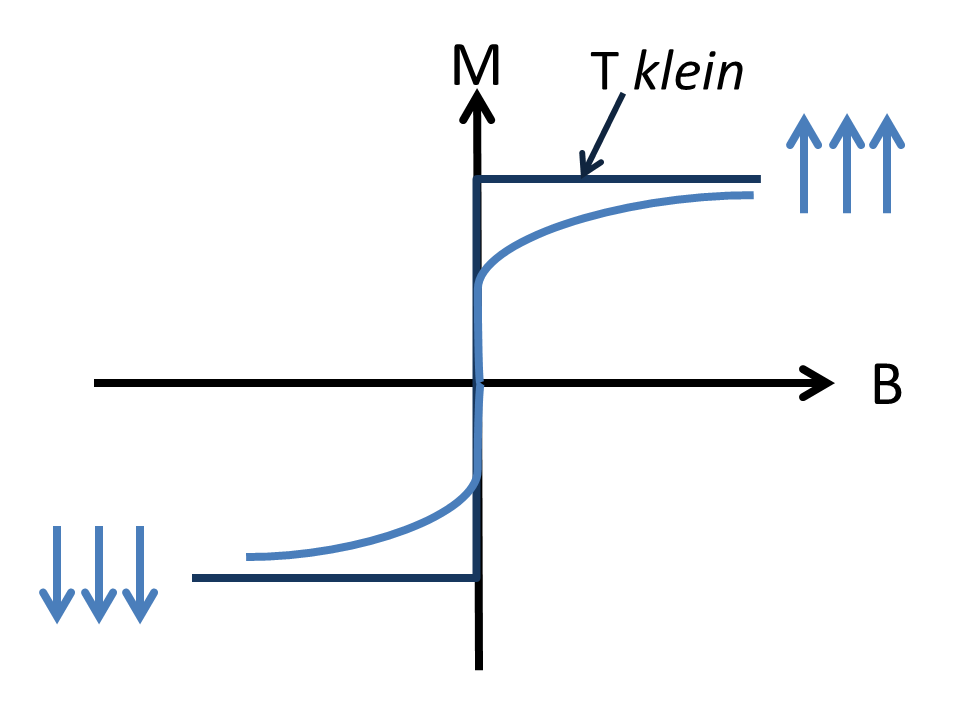
\includegraphics[width=\textwidth]{Folie27.png}
		\caption{Magnetisierung zum Beispiel} 
		\label{fig:Magnetisierung}
		\centering
	\end{subfigure}
	~
\begin{subfigure}[h]{0.5\textwidth}
		\centering
		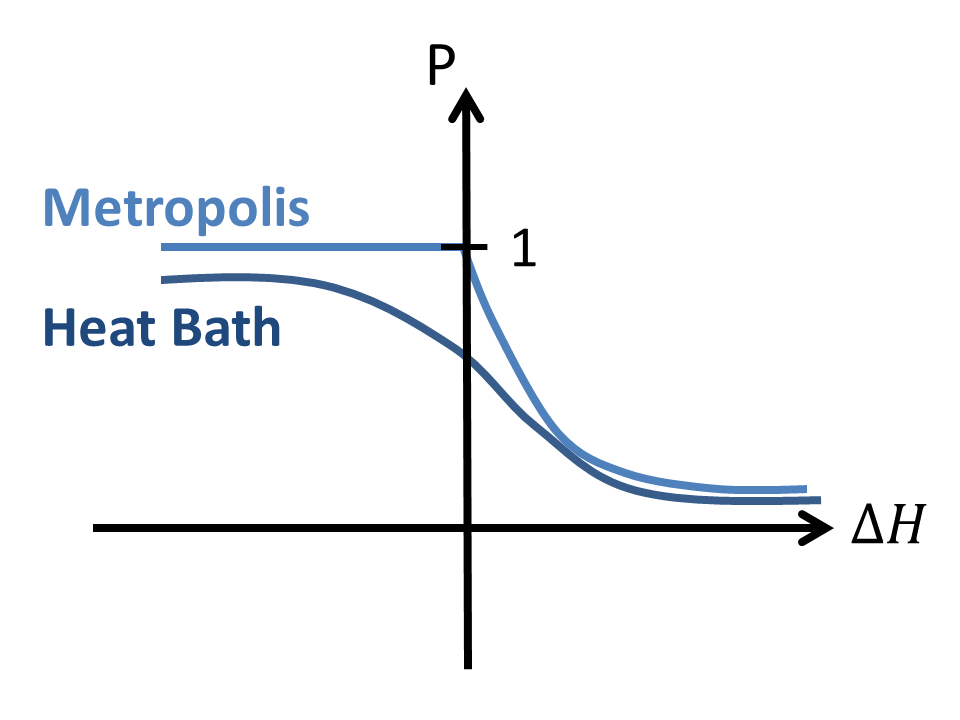
\includegraphics[width=\textwidth]{Folie28.png}
		\caption{Vergleich beider Algorithmen}
		\label{fig:MA_HB}
		\centering
	\end{subfigure}
	\caption{ }
\end{figure}	



Allgemein: N Spins \\
$\Rightarrow \; 2^N$-Zustände ($2^{100} = 10^{30}$) \\
$\Rightarrow$ d.h. durch direktes Summieren numerisch nicht lösbar \\
$\Rightarrow$ Näherungsverfahren!

\subsection{Monte Carlo Simulation}
(Wir rechnen im kanonischen Ensemble die Zustandssumme aus.)
\begin{align}
\langle M \rangle = & \frac{\sum^{2^N}_{\underline{S}} M(\underline{S}) \;  e^{-\beta H(\underline{S} ) }}{\sum^{2^N}_{\underline{S}} e^{-\beta H(\underline{S})}}  
\begin{cases}
 \underbrace{\approx}_{\substack{ \text{simple} \\ \text{sampling}}} 
& \frac{\sum^{k}_{\underline{S}} M(\underline{S}) \; e^{-\beta H(\underline{S})}}{\sum^{k}_{\underline{S}} e^{-\beta H(\underline{S})}} \mbox{ nicht alle } 2^N \mbox{Zust. sondern } k \\
\underbrace{\approx}_{\substack{ \text{importance} \\ \text{ sampling}}} & 
\frac{\sum^{k}_{\underline{S}} M(\underline{S}) \; e^{-\beta H(\underline{S})} \frac{1}{w(\underline{S})}}{\sum^{k}_{\underline{S}} e^{-\beta H(\underline{S})} \frac{1}{w(\underline{S})}}
\end{cases}
\end{align}

Dabei sind $[\underline{S}]$ Konfigurationen von Spins mit Wahrscheinlichkeit $w(S)$. Wähle 

\begin{tcolorbox}[ams gather,title=, colback=blue!10!white, colframe=blue!30!black]  
w(\bar{S})= e^{-\beta H(\underline{S})}  
\end{tcolorbox}
 und dann folgt

\begin{tcolorbox}[ams gather,title=, colback=blue!10!white, colframe=blue!30!black]  
\langle M \rangle = \frac{1}{K} \sum_{ [\underline{S}]}^{(k)} M(\bar{S})
\end{tcolorbox}
$\Rightarrow$ Problem: wir brauchen Zustände $\overline{S}$ mit Wahrscheinlichkeit $w(\overline{S})\propto e^{-\beta H(\overline{S})}$ ($\Rightarrow$Problematisch). Wir brauchen also ein Verfahren das Zustände des Systems (Spinkonfiguration $\underline{S}$) erzeugt die eben dieser eben genannten Wahrscheinlichkeitsverteilung genügt. Wie bekommt man jetzt Konfigurationen mit einer bestimmten Wahrscheinlichkeitsverteilung? 
Lösung: \textbf{ Metropolis-Algorithmus}. \\

Beginne einen Markov-Prozess (Kette)\footnote{meint dass der nächste Zustand nur von seinem Vorgänger abhängt, d.h. ein Zustand wird vom Vorgängerzustand erzeugt} 
\begin{align*}
\underline{S}_0 \rightarrow \underline{S}_1 \rightarrow \underline{S}_2
\end{align*}
(also beispielsweise $\uparrow \uparrow \uparrow \; \rightarrow \; \uparrow \downarrow \uparrow \; \rightarrow \; \uparrow \downarrow \downarrow$)

\begin{enumerate}
\item $\underline{S}_n $ sei ein Zustand
\item \label{Punkt2} erzeuge Versuchszustand \textit{(trial state)} $\underline{S}_r$ durch \textit{geeignete} Veränderung.
\item berechne: 
\begin{align}
r= \frac{w(\underline{S}_r)}{w(\underline{S}_n)} = \frac{e^{- \beta H(\underline{S}_r )}}{e^{- \beta H(\underline{S}_n )}}= e^{-\beta (H(S_r)-H(S_n))}
\end{align}

\item Fallunterscheidung: \\ 
$r>1$: akzeptieren, $\underline{S}_{n+1} = \underline{S}_r$\\
$r \leq 1:$ akzeptieren mit Wahrscheinlichkeit $r$
\item  $\rightarrow$ \ref{Punkt2}.
\end{enumerate}
\textbf{Implementierung:} am Beispiel einer Spinkette $\uparrow \uparrow \uparrow \uparrow \uparrow \uparrow$ (der letzte wechselwirkt wieder mit dem ersten wieder, periodische Randbedingungen also)

\begin{enumerate}
\item Array von Spins \texttt{int Spins}$[N]$: $ +1|+1|+1|+1|+1|+1|$ (mit Anfangsbedingung $S_i =1$)
\item \label{wiederPunkt2} Versuchsschritt: misst \textbf{'single spin flip'}, d.h. ein Spin wird gedreht: \\
$S_i \rightarrow - S_i$: $ +1|-1|+1|+1|+1|+1|$
\item $\Delta H= H(\underline{S}_r)  - H(\underline{S}_n) = 2 J (S_i S_{i-1} + S_i S_{i+1}) + 2BS_i \; \; \Rightarrow r= e^{-\Delta H / k_BT}$
\item \texttt{if (rand()/Randmax $<$r)} $S_r \rightarrow -S_i$
\item $\rightarrow$ \ref{wiederPunkt2}.
\end{enumerate}

\begin{itemize}
\item Wenn alle Spins einmal abgefragt wurden: $1MCS$ (\textbf{M}onte \textbf{C}arlo \textbf{S}chritt) pro Spin
\item Mittelung über viele MCS

\item Zu Beginn der Simulationen ist der Markov Prozess nicht im Gleichgewicht (hängen vom Anfangszustand ab) \\
$\Rightarrow$  die ersten $k$ MCS sollten nicht zur Mittlung herangezogen werden und damit bei der Berechnung von $\langle M \rangle$ weggelassen werden.
 \begin{align}
\langle M \rangle = \frac{1}{(K-k)} \sum_{i=k}^K M_i 
\end{align}
mit der Magnetisierung $M_i$ des $i-$ten Spinlaufs
\begin{align*}
M_i = \frac{1}{N} \sum_{j=1}^N \sigma
\end{align*}
\textbf{Beweis:} Metropolis-Algorithmus erzeugt Konfigurationen $\underline{S}$ mit einer Wahrscheinlichkeitsverteilung von $w(\underline{S}) \propto e^{-\beta H(\underline{S})}$ (Wie betrachtet man denn nun statistische nicht Gleichgewichtsprozesse so wie diesen Markov Prozess?)
\item $w(\bar{S}):$ Wahrscheinlichkeit im Zustand $\underline{S}$ zu sein.
\item Markov $\underline{S} \rightarrow \underline{S'}$ mit $p(\underline{S}, \underline{S'}): $ Wahrscheinlichkeit, im Prozess von $\underline{S}$ nach $\underline{S'}$ zu wechseln

Aufgabe: $p$ bestimmen, sodass $w(\underline{S})$ herauskommt
\end{itemize} %TODO bild mit strichen
\begin{align*}
\Delta w(\underline{S}) =& 
- \sum_{\underline{S'}} w(\underline{S}) \; p(\underline{S} \rightarrow \underline{S'})\quad  \mbox{ \textit{(raus)} } \\
 &+  \sum_{\underline{S'}} w(\underline{S'}) \; p(\underline{S'} \rightarrow \underline{S}) \quad \mbox{\textit{ (rein)} } \\ 
 \overset{!}{=}& 0
\end{align*}

%TODO ising modell: phasenübergang bei 2....irgendwas. Schwankungen in der reduzierten magnetisierung für werte kurz unter 2 kommen durch spezifische Wärmekapazität als schwankung der Energie und genauso die spezifische suszeptibilität als schwankung der Magnetisierung. Die zahl der Montecarlo schritte steigt bis man im gleichgewicht ankommt für steigende werte für T. Sie fällt für höhere werte detulich größer aus bis sie bei Null ankommt

Betrachte eine mögliche Lösung: jeder einzelne Summand wird $=0$. (\textbf{'detailed balance'}).
 \begin{align}
\Rightarrow   w(\underline{S}) \; p(\underline{S} \rightarrow \underline{S}')- w(\underline{S}') \; p(\underline{S}' \rightarrow \underline{S}) =0 
\end{align}
\begin{align}
\Rightarrow  \frac{p(\underline{S} \rightarrow \underline{S}')}{p(\underline{S}' \rightarrow  \underline{S})} = \frac{w(\underline{S}')}{w(\underline{S})} = e^{-\beta(E(\underline{S}')- E(\underline{S})}
\end{align}
\begin{enumerate}
\item \underline{Lösung:} (eigentlich. Metropolis Algorithmus)
 \begin{align}
p(\underline{S} \rightarrow \underline{S}')
\begin{cases}
e^{-\beta(E(\underline{S}')- E(\underline{S})} & \text{ für } \Delta E > 0 \\
1 & \text{ sonst}
\end{cases}
\end{align} 

\item \underline{Lösung:} (\textbf{Heat-bath algorithm})
\begin{align*}
p(\underline{S} \rightarrow \underline{S}') = \frac{1}{1+ e^{\beta \Delta E}} \mbox{, weil } 
\end{align*}

\begin{align*}
\frac{p(\underline{S} \rightarrow \underline{S}')}{p(\underline{S}' \rightarrow \underline{S})} = \frac{1+e^{-\beta \Delta E} }{1+e^{\beta \Delta E}} = \frac{e^{-\beta \Delta E} (e^{\beta \Delta E}+1)}{1+e^{\beta \Delta E}}= e^{-\beta \Delta E}
\end{align*}
\end{enumerate}
Siehe zum Vergleich auch nochmal Abbildung \ref{fig:MA_HB}.



\subsection{Master Gleichung und Monte Carlo Dynamik}
\textit{(Zusammenhang mit irreversibler Dynamik)}\\

\begin{figure}[h] 
		\begin{subfigure}[h]{0.5 \textwidth}
		\centering
		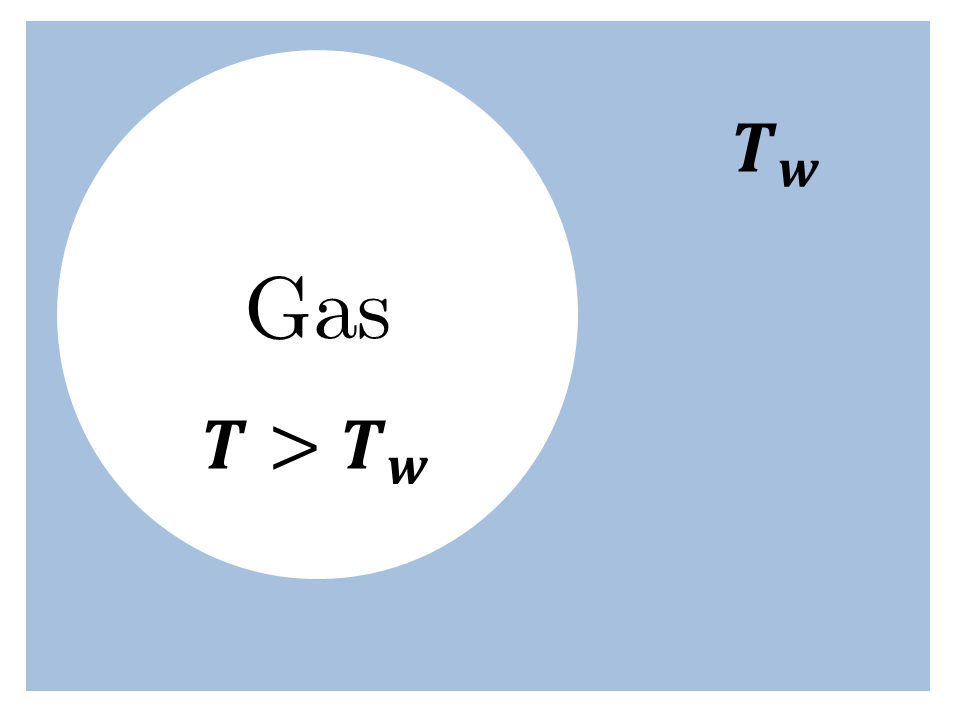
\includegraphics[width=\textwidth]{Folie29.png}
		\caption{Betrachtetes System aus Beispiel} 
		\label{fig:Gassystem}
		\centering
	\end{subfigure}
	~
\begin{subfigure}[h]{0.5\textwidth}
		\centering
		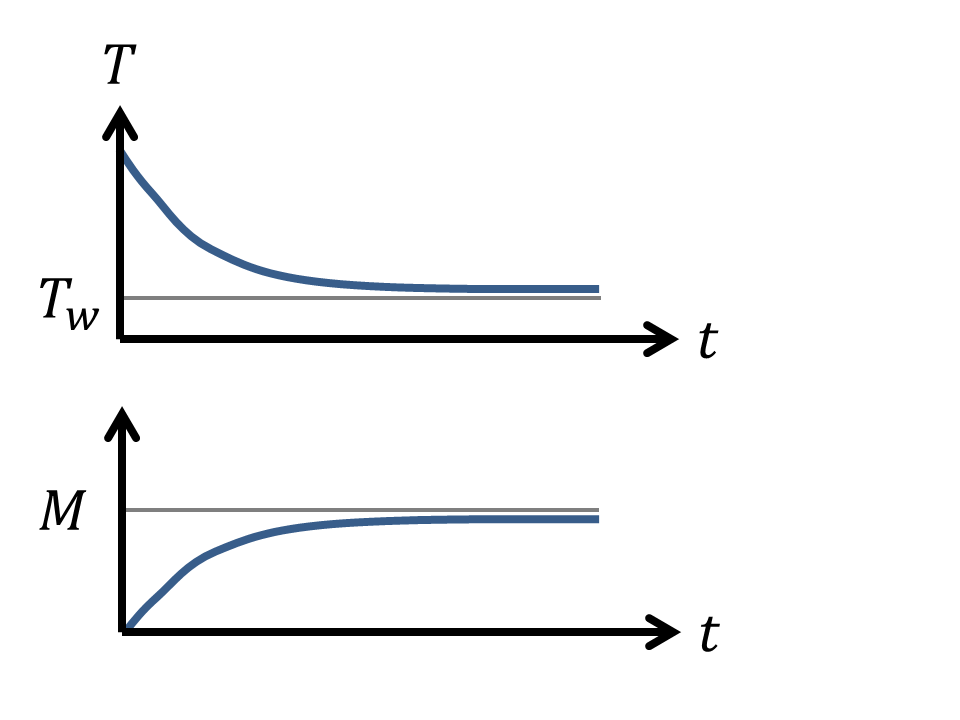
\includegraphics[width=\textwidth]{Folie30.png}
		\caption{(oben) Gas, das mit der Zeit sinkt. \\ (unten) Equibrilierung eines Spinsystems}
		\label{fig:sinken}
		\centering
	\end{subfigure}
	\caption{ }
\end{figure}	



Betrachte ein System im nicht-Gleichgewicht, das equilibriert (irreversibel): 
\textbf{Beispielsweise}
\begin{itemize}
\item ein Gas, das mit der Zeit sinkt (Abb. \ref{fig:Gassystem}, \ref{fig:sinken}).
\item oder ein Spinsystem. (equilibriert durch 'Ankopplung an Phononen', siehe Abbildung \ref{fig:sinken})
\end{itemize}    
Wie beschreibt man solche \textbf{irreversiblen Dynamiken}?
\begin{itemize}
\item Stellen uns vor, wir haben $\infty$ viele Kopien des Systems und machen nun 'Momentaufnahmen' der Zustände über der Zeit. 
\item Berechne nun die zeitliche Änderung der Wahrscheinlichkeit $p_r(t)$ (Wahrscheinlichkeit, das System zur Zeit $t$ im Zustand $r$ zu finden)
\item betrachte quantenmechanisches System im Kontakt mit einem Wärmebad
\begin{align}
\bar{H}_{gesamt} = \underbrace{ \bar{H}}_\text{System} + \underbrace{\bar{H}'}_\text{Wärmebad} + \underbrace{ \bar{H}_i}_\text{Wechselwirkung}
\end{align}
\item System sei im Zustand $r$, $\bar{H} \Psi_r = E_r \Psi_r$ mit Wahrscheinlichkeit $p_r(t)$.
\end{itemize}
\textbf{Master Gleichung}
\begin{align}
\frac{dp_r}{dt}= \sum_s \left( p_s \; w_{sr}  - p_r \; w_{rs} \right) 
\end{align}
mit $ w_{sr}, \;  w_{rs}$ als Übergangsraten. Eine  Anwendung im Wärmebad ergibt
\begin{align}
w_{rs}= & \sum_{r',s'} p_{r'}' w_g(rr' \rightarrow ss') = \frac{1}{Z'} \sum_{r',s'}  e^{-\beta E_{r'}'} w_g (rr' \rightarrow ss') \mbox{ Wärmebad ist kanonisch! } \\
w_{sr}= & \frac{1}{Z'} \sum_{r',s'}  e^{-\beta E_{s'}'} w_g (ss' \rightarrow rr')
\end{align}
\begin{itemize}
\item Energieerhaltung: $E_{r'}' + E_r = E_{s'}' + E_s$ (*)
\item Symmetrie im Gesamtsystem $w_g (rr' \rightarrow ss') = w_g (ss' \rightarrow rr')$(*)
\end{itemize}


aus (*) einsetzen folgt
\begin{align}
w_{sr}&= \frac{1}{Z'} \sum_{r',s'} e^{\beta (E_{r'}' -E_{s'}') } e^{-\beta E_{r'}'}  w_g (rr' \rightarrow ss') = w_{rs} \; e^{-\beta (E_r - E_s)} \\
& \Rightarrow  \frac{w_{sr}}{w_{rs}}= e^{-\beta (E_r - E_s)} \label{Master}
\end{align}
\underline{also:} Irreversible Dynamik eines Systems in Kontakt mit einem Wärmebad wird beschrieben durch Master-Gleichung (unter Verwendung von Formel \ref{Master})
\begin{align}
 \frac{dp_r}{dt}= \sum_s( p_s(t) w_{sr} - p_r(t) w_{rs})
\end{align}
 Diese Dynamik wird durch Metropolis Algorithmus (oder Heat Bath Algorithmus) simuliert. %TODO nicht durch MC?

\begin{figure}[h] 
		\begin{subfigure}[h]{0.5 \textwidth}
		\centering
		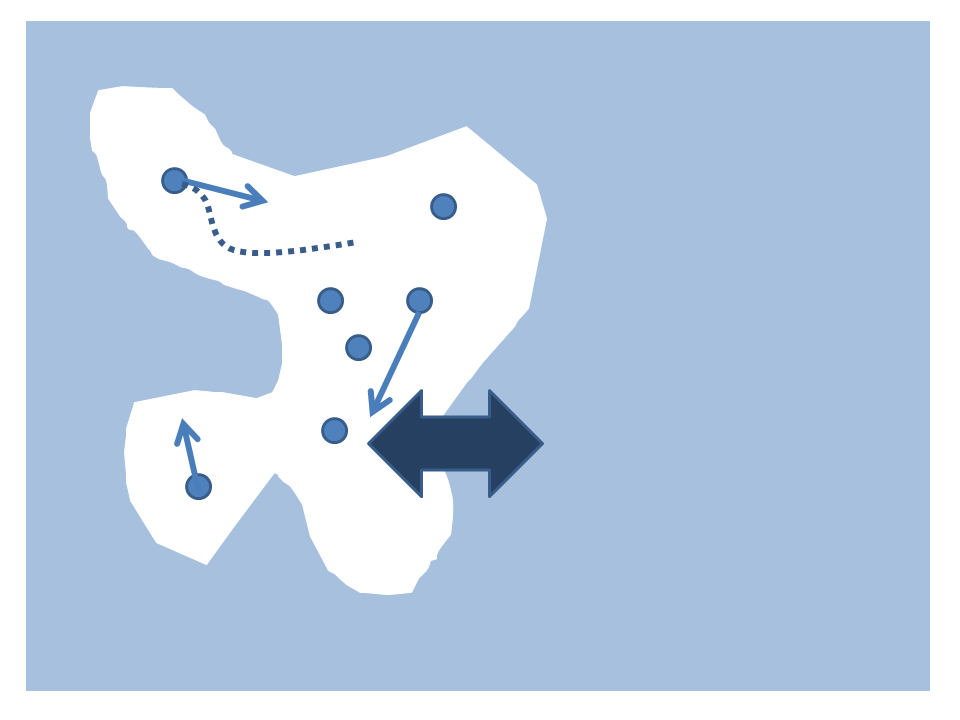
\includegraphics[width=\textwidth]{Folie31.png}
		\caption{betrachtetes System} 
		\label{fig:System}
		\centering
	\end{subfigure}
	~
\begin{subfigure}[h]{0.5\textwidth}
		\centering
		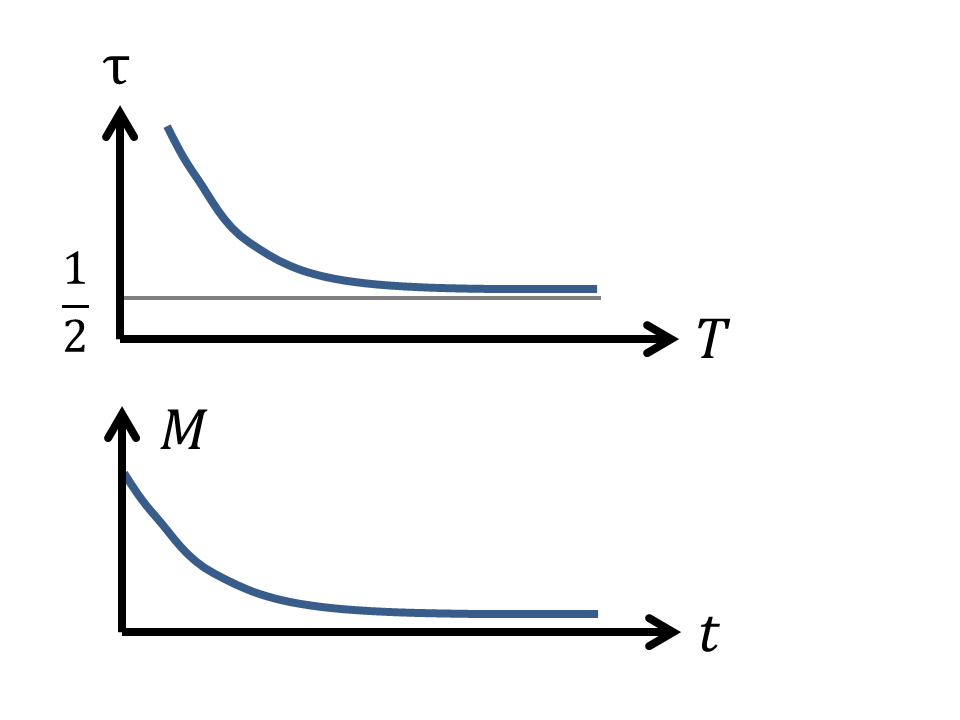
\includegraphics[width=\textwidth]{Folie32.png}
		\caption{Relaxationszeit und Magnetisierung}
		\label{fig:Relax}
		\centering
	\end{subfigure}
	\caption{ }
\end{figure}	

\underline{Beachte:} 
\begin{itemize}
\item $w_{sr}$ liegen nicht absolut fest. Mit $w_{sr}, w_{rs}$ ist auch $\gamma (t) w_{sr}, \gamma(t) w_{rs}$ Lösung \\  $\Rightarrow$ Zeitskala ist nicht absolut festgelegt!
\item $w_{sr}$ ist nicht mikroskopisch bekannt (im Raum nicht festgelegt)
\item Die Master Gleichung beschreibt \textit{ausschließlich} irreversible Dynamiken, nicht aber die Bewegungsgleichung innerhalb des Systems $\tilde{H}$, (Abb. \ref{fig:System})! 
\item speziell für das \textsc{Ising}-Modell heißt diese Dynamik, die durch die Mastergleichung beschrieben wird  \textbf{Glauber-Dynamik}.(Besonders wichtig, das \textsc{Ising}-Modell keine Bewegungsgleichung hat)
\end{itemize}


\textbf{Beispiel:} (Glauber Dynamik für 2 Spins) \\ 
$H=-J S_1 S_2$ mit $S_{1,2} = \pm 1$
$\Rightarrow 2^2 =4$ Zustände: 
\begin{center}
\begin{tabular}{c c c c}
$\uparrow \uparrow$ & $\uparrow \downarrow$ & $\downarrow \uparrow$ & $ \downarrow \downarrow$ \\ 
$++$ & $+-$ & $-+$ & $--$ \\ 
\end{tabular} 
\end{center}

 \begin{align*}
 \frac{dp_{++}}{dt} = \sum_s p_s w_{sr} - p_r w_{rs}
 \end{align*}
 (Energie $++$ und $--$ sind genau gleich, da ja kein externes Feld angelegt ist. Nur interessant ist also der Übergang von $++, --$ zu $+-,-+$) $\Rightarrow$ Annahme: Single spin flip und 'Metropolis' mit 
 \begin{align*}
 w=
 \begin{cases}
 1 & \Delta E <0 \\
 e^{- \frac{\Delta E}{kT}} & \Delta E>0
 \end{cases}
 \end{align*}
 Es gibt 
 \begin{itemize}
 \item  $w_{++ \rightarrow --}= w_{+- \rightarrow -+}$ etc...
 \item $w_{+- \rightarrow ++}= w_{-+ \rightarrow ++}=1$ etc...
 \item $w_{-- \rightarrow -+}= w_{-- \rightarrow +-}= w= e^{-\frac{2J}{k_BT}}$ etc... 
 \end{itemize}
 
  \begin{align*}
 \frac{dp_{++}}{dt} =& \sum_s p_s w_{s r} - p_{r} w_{r s} \\
 =& p_{+-} w_{+- \rightarrow ++} - p_{++} w_{++ \rightarrow +-} +
 p_{-+} w_{-+ \rightarrow ++} - p_{++} w_{++ \rightarrow -+} =
 p_{+-} + p_{-+} - 2 p_{++} w \\
 \frac{dp_{--}}{dt}= & p_{+-} + p_{-+} - 2p_{--}w \\
  \frac{dp_{+-}}{dt}= & p_{++}w + p_{--} w- 2p_{+-} \\
   \frac{dp_{-+}}{dt}= & p_{++}w + p_{--}w -2p_{-+}
 \end{align*}
$\Rightarrow$ homogenes, lineares Gleichungssystem \\
$\Rightarrow$ Lösung für $\lambda$ mit 
\begin{align*}
\begin{vmatrix}
-2w+\lambda & 0 & 1 & 1 \\
0 & -2w +\lambda & 1 & 1 \\
w & w & -2w + \lambda & 0 \\
w & w & 0 & -2+\lambda 
\end{vmatrix} 
\end{align*}
\begin{align*}
\Rightarrow \lambda_1=0, \lambda_2=2, \lambda_3=2w+2, \lambda_4=2w \end{align*}

\textbf{Wichtig:} Kleinstes $\lambda >0$ definiert die Relaxationszeit! \\
$\Rightarrow$ für lange Zeiten: 
\begin{align*} p_s(t) \approx a_s + b_s e^{-\lambda_4 t} \approx a_s + b_s e^{-\frac{t}{\tau}} \quad \quad \left(\text{mit} \tau= \frac{1}{20}= \frac{e^{2J/k_BT}}{2} \right)
\end{align*}

\textbf{Magnetisierung:} 
\begin{align}
M(t)= \sum_s p_s(t) M_s = p_{++}(t) + p_{--}(t) \underbrace{\approx}_{t \to \infty} M_0 \; e^{-\frac{t}{\tau}} + \underbrace{const}_{=0}
\end{align}


\underline{Diskussion:}  (siehe auch Abb. \ref{fig:Relax})
\begin{itemize}
\item $\tau$ hängt vom 'Algorithmus' ab (siehe auch Grenze für $T\to \infty $)
\item $p(t)$ hängt von Annahmen bezüglich Übergangswahrscheinlichkeitsraten  also der Dynamik ab (single spin flip oder nicht)
\end{itemize}
\subsection{Phasenübergange und Skalentheorie}

\begin{figure}[h] 
		\begin{subfigure}[h]{0.5 \textwidth}
		\centering
		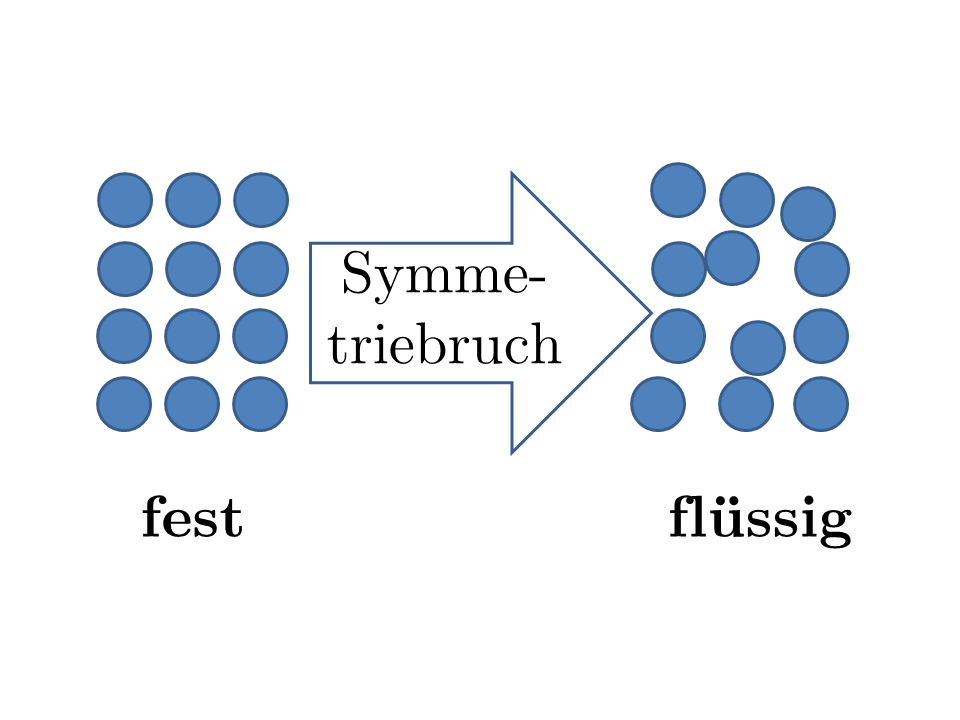
\includegraphics[width=\textwidth]{Folie33.png}
		\caption{Symmetriebruch beim Phasenübergang} 
		\label{fig:Symmetriebruch}
		\centering
	\end{subfigure}
	~
\begin{subfigure}[h]{0.5\textwidth}
		\centering
		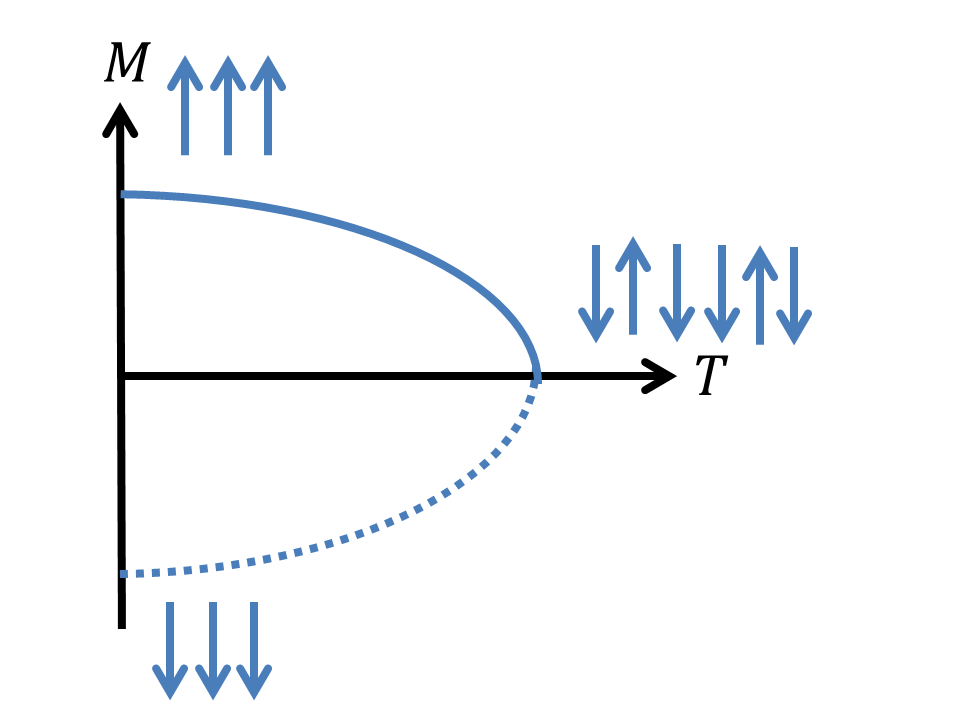
\includegraphics[width=\textwidth]{Folie34.png}
		\caption{Computer: \textsc{Ising}-Modell}
		\label{fig:Computer}
		\centering
	\end{subfigure}
	\caption{ }
\end{figure}	

Ideale Gase haben keine Wechselwirkung erst die Wechselwirkung zwischen Teilchen erklärt aber das Entstehen von Ordnung. Ordnung entsteht häufig spontan durch Phasenübergänge, bei dem eine Symmetrie gebrochen (Abb. \ref{fig:Symmetriebruch}) wird. Ein Analytisch lösbares Modell für das Studium von Phasenübergängen ist das in Abb. \ref{fig:Computer} dargestellte \textbf{ (2d) \textsc{Ising}-Modell}: 

Ordnungsparameter: 
\begin{align*}
 \lim\limits_{\substack{B \to 0 \\ N \to \infty}} M(B)
\end{align*}

\textbf{Analytisch:}  (2D, Quadratgitter mit $B=0$ und $N \to \infty$) 
\begin{align}
H= - \underbrace{ \sum_{i,j}}_{\substack{\text{ 4 nächste} \\ \text{Nachbarn}}} \frac{J}{2}\sigma_i \sigma_j \; , \quad \quad \sigma_i=\pm 1
\end{align}
Die exakte Lösung von Onsager (1944) erhielt einen Nobelpreis. Heutzutage löst man es jedoch auf andere Weise, beispielsweise
\begin{itemize}
\item[-] graph theory
\item[-] transfermatrix methods
\end{itemize} 

\begin{figure}[h] 
		\begin{subfigure}[h]{0.5 \textwidth}
		\centering
		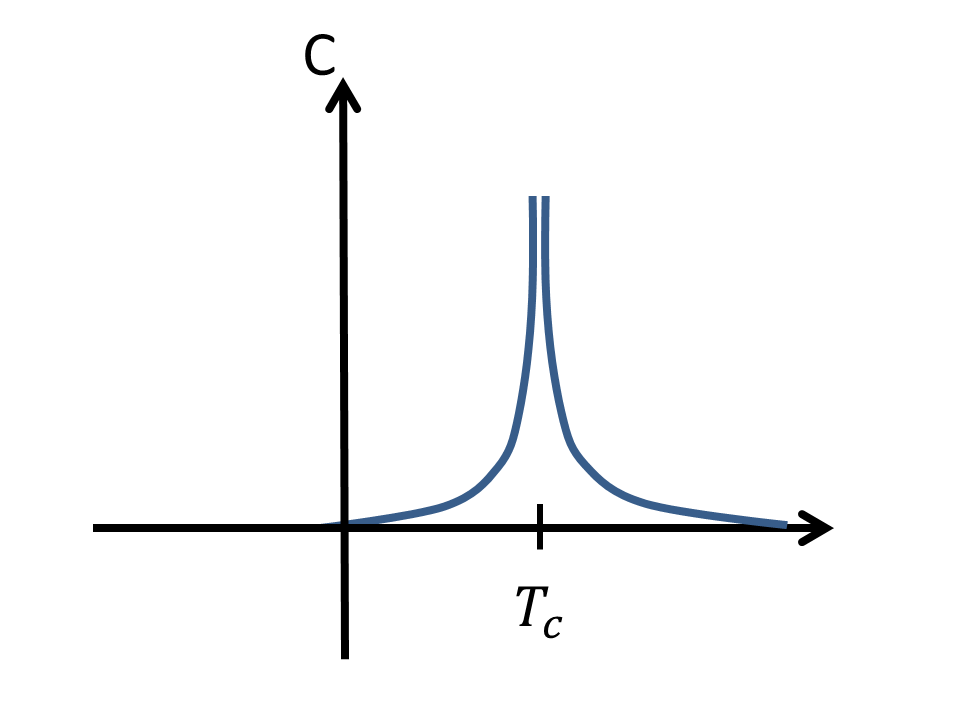
\includegraphics[width=\textwidth]{Folie35.png}
		\caption{Singularität bei der kritischen Temperatur} 
		\label{fig:Singularity}
		\centering
	\end{subfigure}
	~
\begin{subfigure}[h]{0.5\textwidth}
		\centering
		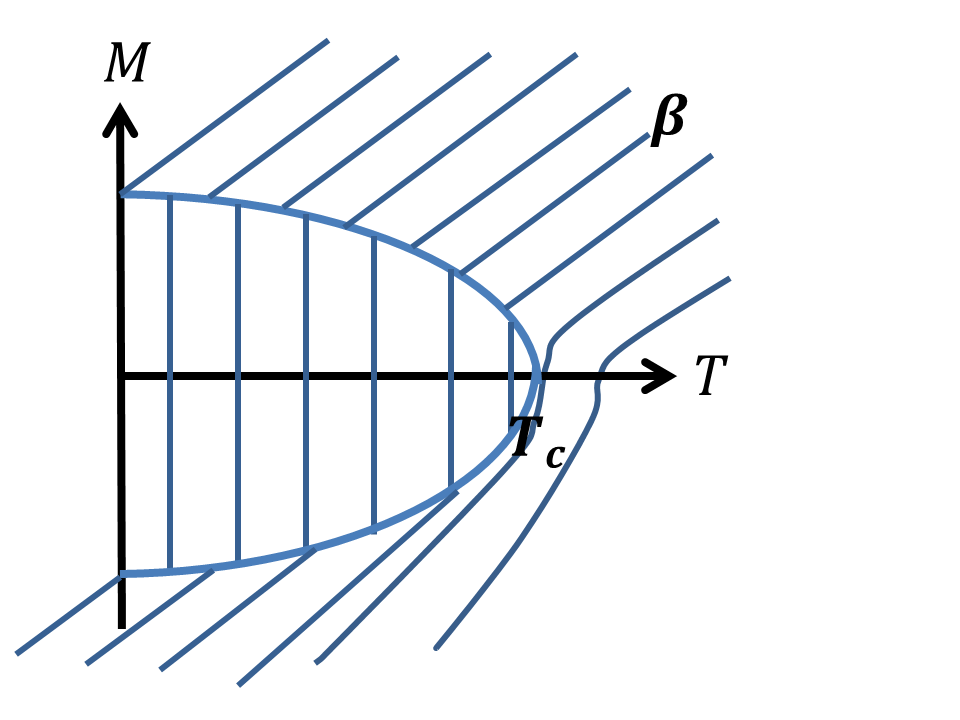
\includegraphics[width=\textwidth]{Folie36.png}
		\caption{\textsc{Ising}-Modell im Feld.}
		\label{fig:IsingmodellimFeld}
		\centering
	\end{subfigure}
	\caption{ }
\end{figure}	

\textbf{innere Energie:}
\begin{align}
\frac{U}{N}= - J \; coth\left( \frac{2J}{k_BT}\right) \left[ 1 + \frac{2}{\pi} \left( 2 \; tanh^2 \left( \frac{2J}{k_BT} \right) - 1 \right) K_1(\kappa ) \right]
\end{align}
mit
\begin{align}
\kappa= \frac{2 \; sinh \left( \frac{2J}{k_BT} \right)}{cosh^2 \left( \frac{2J}{k_BT} \right) } \; , \; K_1(\kappa)= \int_0^\frac{\pi}{2} \frac{1}{\sqrt{1- \kappa^2 \; sinh^2(\Phi)}} d\Phi
\end{align}
U ist nicht analytisch bei einer Temperatur $T_c$ mit 
\begin{align*}
sinh \left(\frac{2J}{k_BT_c} \right) = 1\quad \Rightarrow cosh \left(\frac{2J}{k_BT_c} \right)= \sqrt{2} \quad \Rightarrow 2 tanh^2\left( \frac{2J}{k_B T_c}\right) =1
\end{align*}
 mit $k_B T_c = 2.269 J$.
 Beachte, dass $K_1(\kappa)$ hat eine Singularität (Abb. \ref{fig:Singularity}) für $\kappa \to 1$:
 \begin{align*}
 K_1(\kappa) \propto  ln \left(\frac{U}{\sqrt{1-\kappa^2}} \right)
 \end{align*}
 $U$ bleibt endlich, aber seine Ableitung divergiert. Typisch für einen Phasenübergang sind unter anderem kritische Punkte mit nicht-analytischen Singularitäten sowie auch Werte hüpfen oder divergieren können. (kritisches Verhalten) Beispielsweise:
\begin{itemize}
\item[•] Dies spezifische Wärme $c(\underbrace{T \to T_c}_{\kappa \to 1}) \propto - ln \left(\vert 1- \frac{T}{T_c}\vert \right)$
\end{itemize}
Der Ordnungsparameter jedoch bleibt endlich. (Magnetisierung:)
\begin{itemize}
\item[•] Magnetisierung 
\begin{align}
m=
\begin{cases}
0 & T>T_c \\
\frac{\sqrt[4]{1+x^2} \sqrt[8]{1-6x^2 +x^4} }{\sqrt{1-x^2}}& T<T_c
\end{cases} \quad \quad \quad \mbox{ wobei } 
\begin{cases}
x= e^{- \frac{2J}{k_B T}}, \\
 x_c=  e^{- \frac{2J}{k_B T_c}} = \sqrt{2} -1
 \end{cases}
\end{align}
\end{itemize}

\textbf{Kritische Exponenten} \\
\textsc{Ising}-Modell mit Feld. (s. Abb. \ref{fig:IsingmodellimFeld})
\begin{itemize}
\item[•] Phasenübergang $1.$Ordnung bei %TODO missing word
des Feldes $\Rightarrow$ \textit{Hysterese}, Ordnungsparameter stetig, kritische Exponenten

\item[•] kritischer Punkt: $B=0, \; (T= T_c) \;  \widehat{=}$ Phasenübergang 2.Ordnung $\widehat{=} $ 2. Ableitung der freien Energie unstetig (z.B. spezifische Wärme) %TODO missing word
sind viele Größen nicht-analytisch. 
\end{itemize}
\begin{figure}[h] 
		\begin{subfigure}[h]{0.5 \textwidth}
		\centering
		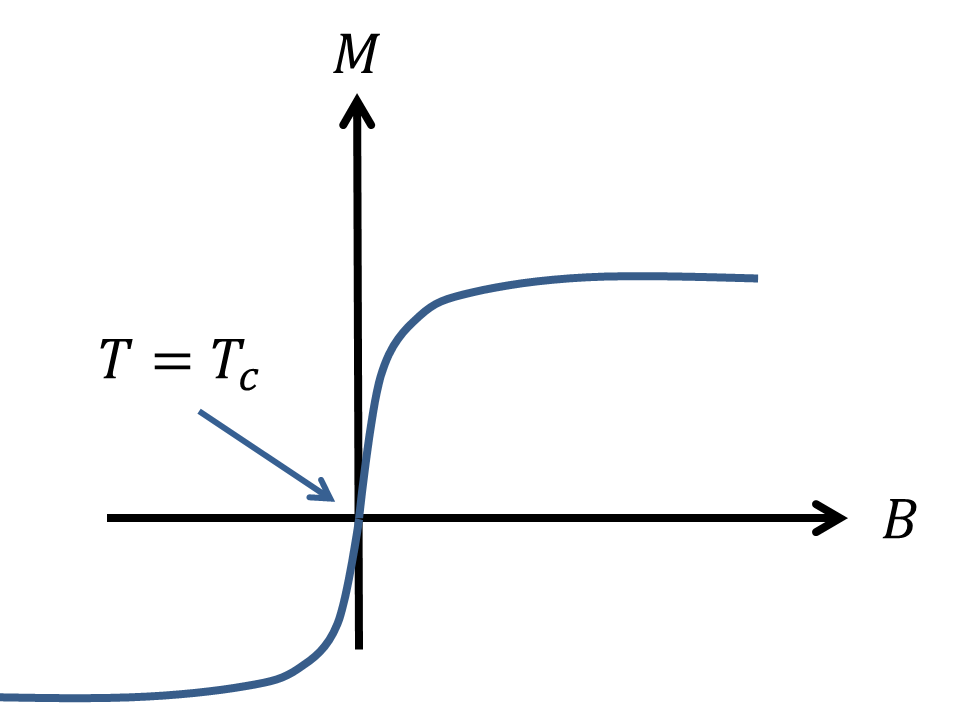
\includegraphics[width=\textwidth]{Folie37.png}
		\caption{} 
		%\label{fig:Symmetriebruch}
		\centering
	\end{subfigure}
	~
\begin{subfigure}[h]{0.5\textwidth}
		\centering
		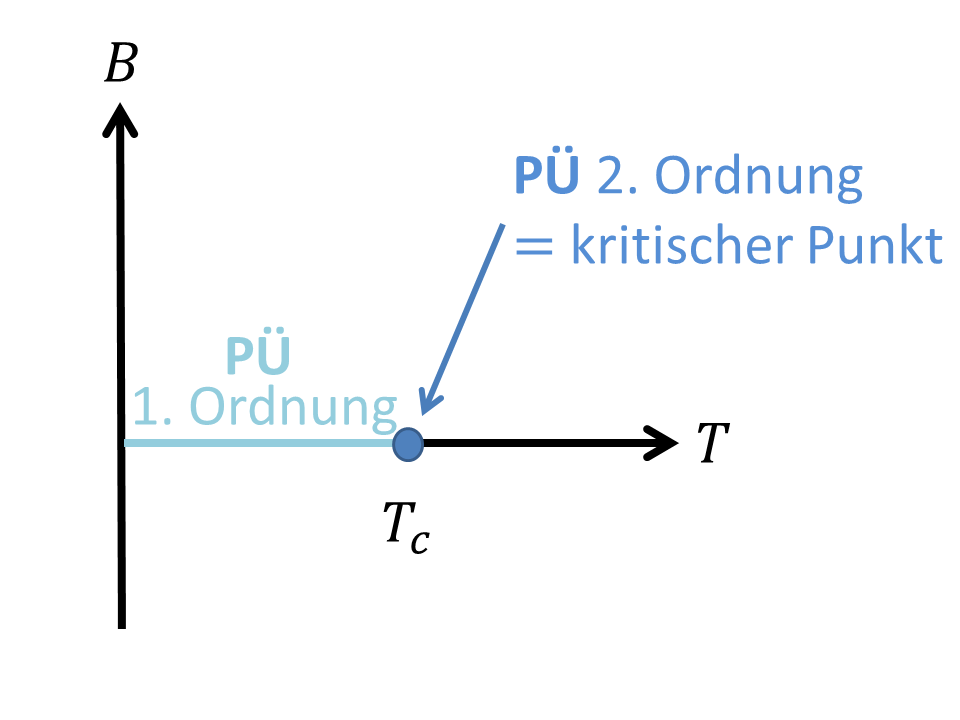
\includegraphics[width=\textwidth]{Folie38.png}
		\caption{}
		%\label{fig:Computer}
		\centering
	\end{subfigure}
	\caption{ Phasendiagramm und kritische Punkte} \label{Phasendiagramm}
\end{figure}	
\textbf{Definition:} Kritische Exponenten beschreiben das Verhalten in der Nähe des kritischen Punktes $(\epsilon = \frac{T - T_c}{T_c} , \;  B) = (0,0)$  ($\widehat{=}$ Abstand vom kritischen Punkt.) Siehe auch Abb. \ref{Phasendiagramm}.
\begin{itemize}
\item $T>T_c, \; B=0 : $ 
\begin{itemize}
\item[•] $c \propto \epsilon^{-\alpha}$ \textit{(spezifische Wärme)}
\item[•] $\chi \propto \epsilon^{-\gamma}$ \textit{(Suszeptibilität)}
\item[•]$\xi \propto \epsilon^{-\nu}$ \textit{(Korrelationslänge)}
\end{itemize}

\item $T<T_c, \; B=0 :$
\begin{itemize}
\item[•] $c \propto \vert \epsilon \vert ^{-\alpha}$ 
\item[•] $\chi \propto \vert \epsilon \vert ^{-\gamma}$
\item[•]$\xi \propto \vert \epsilon \vert ^{-\nu}$ 
\end{itemize}

\item $T=T_c, \; B \to 0:$ siehe \textit{(Magnetisierung)}

\item $+$ eventuelle weitere...
\end{itemize}
  
Magnetisierung (OP) \begin{align}
m= \begin{cases}
M \propto \vert E \vert ^{-\beta} & T<T_c \\
M \propto \vert B \vert ^\frac{1}{\delta} & T=T_c
\end{cases}
\end{align}
Kritische Exponenten beschreiben das führende nicht-analytische Verhalten einer Funktion. Genauer:
\begin{align*}
A(\epsilon)= 
\underbrace{ A_0 + A_1\;  \epsilon + A_2 \; \epsilon +...}_\text{analytisch} 
+ \underbrace{ A_3 \; \epsilon^{0.8}}_{\substack{ \text{führend} \\ \text{ nichtanalytisch} \\ \text{ (kritisch)} }}
+ \underbrace{ A_4 \epsilon^{1.7}}_\text{Korrekturen}
\end{align*}
\begin{align*}
\to A(\epsilon ) \propto A > \epsilon^{0.8}
\end{align*}
Kritische Exponenten haben Eigenschaften, die sie interessant machen:
\begin{enumerate}
\item[1)] Sie sind nicht unabhängig, d.h. es gibt sogenannte Skalengesetze %TODO words missing! 
\item[2)] Universalität, Werte hängen nur von räumlicher Dimension und Symmetrie des Hamiltonoperators ab und nicht von Stärke der Wechselwirkungen, ...
\end{enumerate}

Moderne Theorie der Phasenübergänge 2.Ordnung: \\
Verschiedene physikalische Systeme können dieselben kritischen Exponenten aufweisen! %TODO kommt dieser satz hier hin?
Bestimmung der kritischen Exponenten aus:
\begin{enumerate}
\item[a)] exakte Lösung (2d-\textsc{Ising}-Modell)
\item[b)]Reihenentwicklung
\item[c)]Computersimulation
\item[d)]Experimente
\end{enumerate}
$\Rightarrow$ Bestätigung des Konzepts der Universalität. Beweis später, zunächst werden Beziehungen zwischen den Exponenten hergeleitet. Die Folgen aus: \\
\textbf{Skalenhypothese:}  (\textsc{Widom, Griffith} 1965) als Postulat \\
Freie Energie ist eine verallgemeinerte, homogene Funktion der Variablen $\epsilon, B$:
 \begin{align}
G(a^{x_1} B, a^{x_2} \epsilon)= a \; G(B, \epsilon) \quad \quad \forall a > 0 \label{SkalenHypothese}
\end{align} 
für führenden nicht-analytischen Anteil. Gültig in unmittelbarer Nähe des kritischen Punktes $(\epsilon, B) =0$ für den singulären Anteil der freien Energie. Beachte, dass $G$ eine gerade Funktion von $B$ ist, $\epsilon = \frac{T-T_c}{T_c}$ kann beide Vorzeichen haben!\\
\textbf{Beispiel:}
\begin{align*}
f(x) = x^{0.5} \quad & \Leftrightarrow \quad f(bx) = (bx)^{0.5} = b^{0.5} \; x^{0.5} \\
b= y^2 \quad 
\end{align*}
\begin{tcolorbox}[ams gather,title=, colback=blue!10!white, colframe=blue!30!black] 
 f(a^2 x) = a \; x^{0.5} = a f(x)
 \end{tcolorbox}
'Normal' wäre: f analytisch
\begin{align*}
f(x) &= f(0) + f'(0)x + .... \\
 \Delta f(x) &= f(x) - f(0) = f'(0)x+... \\
\Delta f(ax) &= f'(0) ax +... 
\end{align*} 

\begin{tcolorbox}[ams align,title=, colback=blue!10!white, colframe=blue!30!black] 
\Delta f(ax) &= a\;  \Delta f(x)
\end{tcolorbox}
\textit{Erinnerung an 'Thermodynamik'} \\

\begin{figure}[h] 
		\begin{subfigure}[h]{0.5 \textwidth}
		\centering
		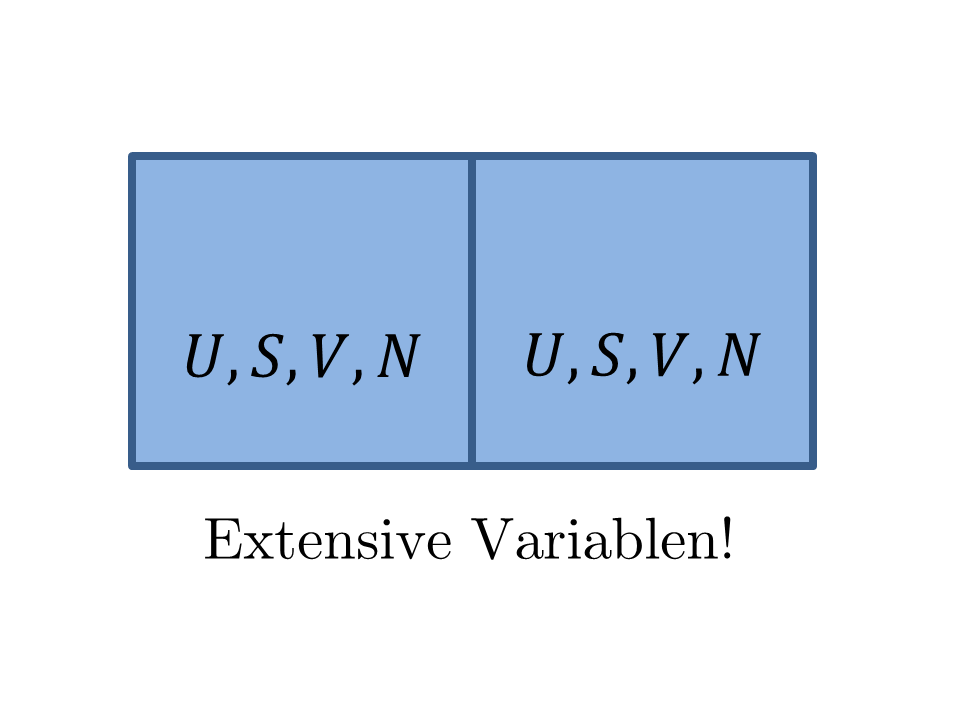
\includegraphics[width=\textwidth]{Folie39.png}
		\caption{Betrachtetes thermodyn. System} 
		\label{fig:Erinnerung}
		\centering
	\end{subfigure}
	~
\begin{subfigure}[h]{0.5\textwidth}
		\centering
		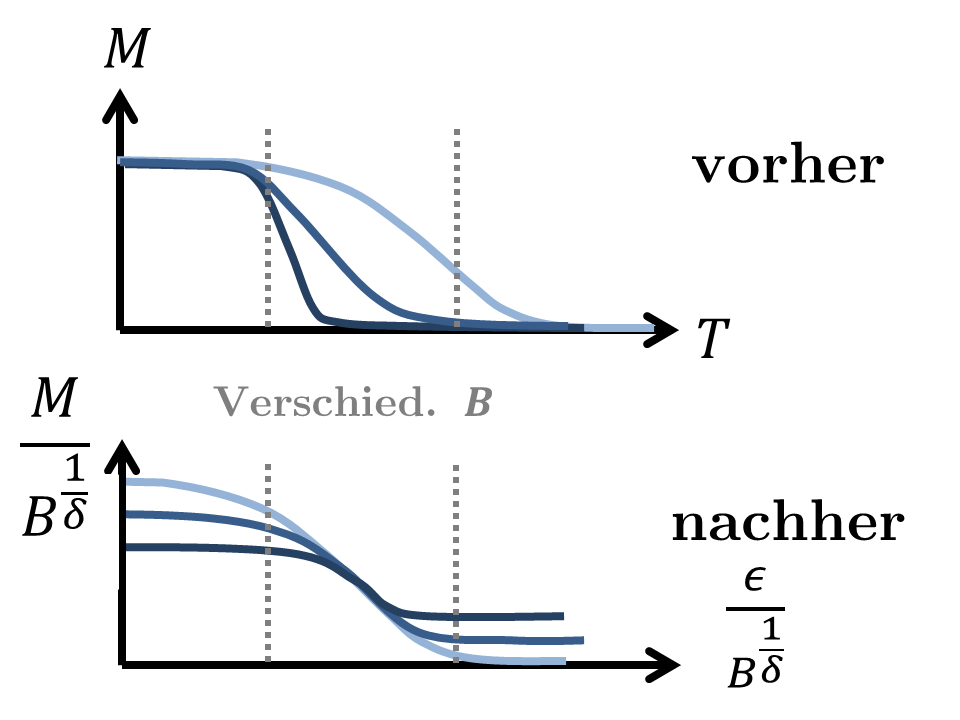
\includegraphics[width=\textwidth]{Folie40.png}
		\caption{scaling plot}
		\label{fig:scalingplot}
		\centering
	\end{subfigure}
	\caption{ }
\end{figure}	

\textit{Wir verdoppeln ein System, gem. Abbildung \ref{fig:Erinnerung},  sodass 
\begin{align*}
\begin{rcases}
U_{ges}= 2U \\
V_{ges} = 2V \\
N_{ges} = 2N \\
S_{ges} = 2S 
\end{rcases}
\quad  \mbox{ also } U(2S, 2V, 2N) = 2 U (S,V,N)
\end{align*}
allgemein
\begin{align*}
U( \lambda S, \lambda V, \lambda N) = \lambda U(S,V,N))
\end{align*}
die innere Energie $U$ ist eine homogene Funktion $1.$Grades!} \\

\textbf{Folgerungen aus der Skalenhypothese (\ref{SkalenHypothese}):} \\
setze $ a= \vert \epsilon \vert ^{-1/x^2}$
\begin{align}
\Rightarrow G\; (\vert \epsilon \vert ^{-\frac{x_1}{x_2}} \;  B, \underbrace{ \frac{\epsilon}{\vert \epsilon \vert}}_{\substack{ +1 \; (T>T_c) \\ -1 \; (T<T_c)}} ) \; = \; \vert \epsilon \vert^\frac{-1}{x^2} \; G(B, \epsilon)
\end{align}
\textbf{Definition:} Skalenfunktion: 
\begin{align}
f^\pm \left( \frac{B}{\vert \epsilon \vert ^\frac{x_1}{x_2}} \right) = G \left( \epsilon^{-\frac{x_1}{x_2}} \; B, \pm 1 \right)
\end{align} 
\underline{Skalenhypothese:}
\begin{align}
G(B,\epsilon) &= \vert \epsilon \vert ^\frac{1}{x_2} \; f^\pm \left( \frac{B}{\vert \epsilon \vert ^\frac{x_1}{x_2}} \right) \\
G(B,\epsilon) &= \vert B \vert ^\frac{1}{x_1} \; g^\pm \left( \frac{\epsilon}{\vert B \vert ^\frac{x_2}{x_1}} \right)
\end{align}
Letztere Gleichung erhält man durch tauschen von $(\epsilon, x_2)$ mit $(B,x_1)$. Außerdem ist
\begin{align*}
g^\pm \left( \frac{\epsilon}{\vert B \vert ^\frac{x_2}{x_1}} \right) = G\left( \frac{B}{\vert B \vert }, \; \frac{\epsilon}{\vert B \vert^\frac{x_2}{x_1}}\right)
\end{align*}
da $G$ eine gerade Funktion von $B$ ist, ist $\pm$ überflüssig.\\

\textbf{Eigenschaften der Skalenfunktionen $g,f$:} \\
G soll am kritischen Punkt ($B\to 0, \; \epsilon \to 0$) endlich bleiben\\
$\Rightarrow f^\pm (0)$ und $g(0)$ bleiben endlich (und ihre Ableitungen) \\
$\Rightarrow \alpha, \beta, \gamma, \delta$ lassen sich durch $x_1, x_2$ ausdrücken: \\
\begin{itemize}
\item \textbf{spezifische Wärme:} \begin{align}
G(0, \epsilon) &= \vert \epsilon \vert
^\frac{1}{x_2}\;  f^\pm (0) \quad \quad \quad  (B=0) 
\end{align}
\begin{align}
&\Rightarrow \;  c \; \propto \;  \frac{\partial^2 G}{\partial \epsilon^2} \; \propto \; \vert \epsilon \vert ^{\frac{1}{x_2}-2} \; = \; \vert \epsilon \vert ^{-\alpha}  \\
& \Rightarrow \;  \alpha = 2- \frac{1}{x_2} 
\end{align}
(Die Exponenten sind allgemein auf beiden Seiten gleich.)

\item \textbf{spontane Magnetisierung:} 
\begin{align}
M(0,\epsilon) \;  \propto \;  \frac{\partial G(B, \epsilon)}{\partial B} \Biggr\vert_{B \to 0} \propto \; \frac{\partial }{\partial B} \Biggr\vert_{B \to 0}  
 \vert \epsilon \vert ^\frac{1}{x_2} f^\pm \left(\frac{B}{\vert \epsilon \vert ^\frac{x_1}{x_2}} \right) \propto \; \vert \epsilon \vert ^\frac{1}{x_2} \frac{1}{\vert \epsilon \vert ^\frac{x_1}{x_2}} \; \propto \;  \vert \epsilon \vert ^\beta 
 \end{align}
 \begin{align}
 \Rightarrow \beta = \frac{1-x_1}{x_2}
\end{align}
\item \textbf{Suszeptibilität:}
\begin{align}
\chi = \frac{\partial M}{\partial B} \Bigg\vert_{B \to 0}
 \propto \vert \epsilon \vert ^\frac{1}{x_2} \frac{1}{\vert \epsilon \vert ^\frac{2 x_1}{x_2}} = \vert \epsilon \vert ^\gamma \quad \quad \Rightarrow \gamma = \frac{2x_1 -1}{x_2}
\end{align}
\item \textbf{Magnetisierung:} (für $\epsilon =0$)
\begin{align*}
G(B, 0 ) = \vert B \vert ^\frac{1}{x_1} \; g\left( \frac{E}{\vert B \vert^\frac{x_1}{x_2}} \right)
\end{align*}
\begin{align}
M \; \propto \;  \frac{\partial G(B,0)}{\partial B} \; \propto \; \vert B \vert ^{\frac{1}{x_1} - 1}
\end{align}
\end{itemize}
Da sich $\alpha, \; \beta, \; \gamma, \; \delta$ (die sogenannten \textit{thermischen Exponenten}) durch $x_1, \; x_2$ ausdrücken lassen, gibt es offensichtlich Zusammenhänge. Mann nennt sie die \\
\begin{itemize}
\item \textbf{Skalengesetze:}
\begin{align*}
\underbrace{\alpha = 2 - \frac{1}{x_2} \quad \quad \quad \quad \beta = \frac{1- x_1}{x_2} \quad \quad \quad \quad \gamma = \frac{2x_1 - 1}{x_2}} 
\end{align*}
\begin{tcolorbox}[ams gather,title= Rushbrooke-Gleichung, colback=blue!10!white, colframe=blue!30!black]  
\alpha + 2 \beta + \gamma = 2 
\end{tcolorbox}

und \begin{align*}
\delta= \frac{x_1}{1-x_1}  \quad \quad \Rightarrow \delta - 1 = \frac{x_1 - 1 + x_1}{1 - x_1} = \frac{2 x_1 - 1}{1 - x_1}
\end{align*}
\begin{tcolorbox}[ams gather,title= Widom-Gleichung, colback=blue!10!white, colframe=blue!30!black] 
\gamma = \beta \; (\delta - 1)
\end{tcolorbox}
\end{itemize}
Weitere Folgerungen sind
\begin{itemize}
\item \textbf{magnetische Zustandsgleichung:}
\begin{align}
M(B,\epsilon)& = - \frac{\partial G}{\partial B} = - \frac{\partial}{\partial B} \left[ \vert B \vert ^\frac{1}{x_1} \; g\left( \frac{\epsilon}{\vert B \vert ^\frac{x_2}{x_1}} \right) \right] \\
&= - B^{\frac{1}{x_1}-1} \; g\left( \frac{\epsilon}{B^\frac{x_2}{x_1}}\right) - \vert B \vert ^\frac{1}{x_1} \; \frac{x_2}{x_1} \; \frac{\epsilon}{\vert B \vert ^{\frac{x_2}{x_1}+1} }  \; \; g'\left( \frac{\epsilon}{\vert B \vert ^\frac{x_2}{x_1} }\right) \\
&= - B^{\frac{1}{x_1}-1} \left[ 
g\left( \frac{\epsilon}{B^\frac{x_2}{x_1}}\right) 
- \frac{x_2}{x_1} \; \frac{\epsilon}{\vert B \vert ^{\frac{x_2}{x_1}} } \; \;g'\left( \frac{\epsilon}{\vert B \vert ^\frac{x_2}{x_1} }\right) \right] 
\end{align}
\begin{tcolorbox}[ams gather,title=, colback=blue!10!white, colframe=blue!30!black] 
M(B,\epsilon)= B^\frac{1}{\delta} \; \; \tilde{g} \left( \frac{\epsilon}{B^\frac{1}{\beta \delta}} \right)   \label{Magnetisierung}
\end{tcolorbox}
\begin{align}
M(B,\epsilon)
= \underbrace{B^\frac{1}{\delta}}_{ \substack{ \text{Grösse hängt} \\ \text{ von einem Feld} \\ \text{ab}}} \cdot \; \text{\~{g}} \Big( \frac{\epsilon}{\underbrace{ B^\frac{1}{\beta \delta}}_{ \substack{ \text{hängt von} \\ \text{zwei Feldern} \\ \text{ ab}}}} \Big) 
\end{align} 
\begin{align*}
\mbox{vorher: } \; & M = M(B,\epsilon) \quad \text{ \textbf{eine} Größe hängt ab von \textbf{zwei} Parametern }\\
\mbox{jetzt: }\; & M = M(B,\epsilon) \quad \text{ \textbf{eine} Größe hängt ab von \textbf{einem} Parameter}
\end{align*}
Dies führt zum sogenannten \textbf{scaling plot}, der in Abbildung \ref{fig:scalingplot} zu finden ist. \\

\begin{figure}[h] 
		\begin{subfigure}[h]{0.5 \textwidth}
		\centering
		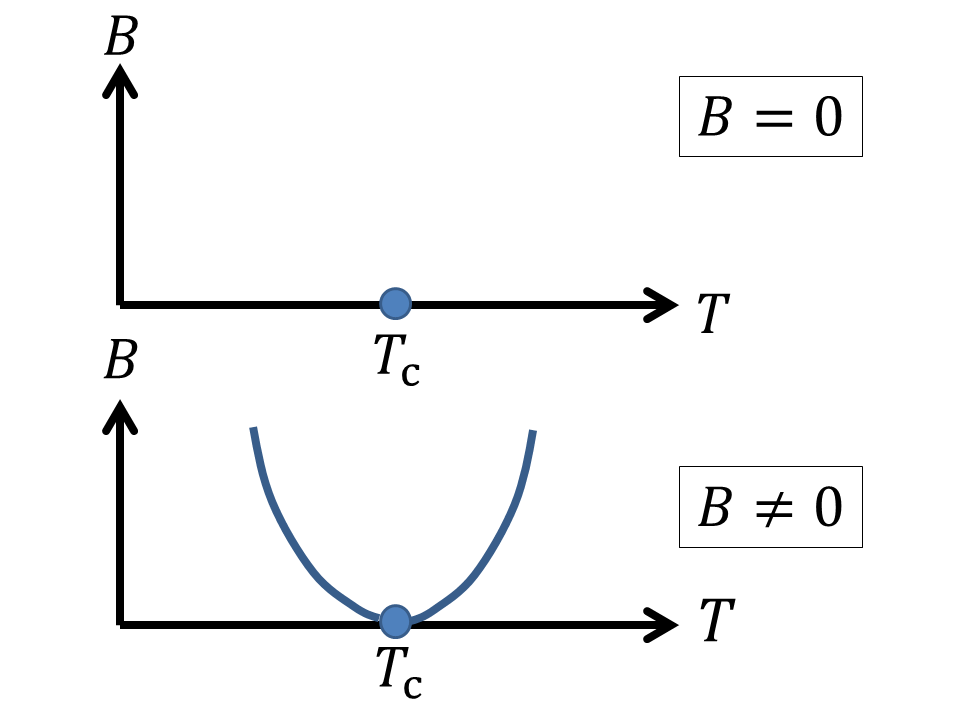
\includegraphics[width=\textwidth]{Folie41.png}
		\caption{Skalenverhalten der freien Energie} 
		\label{crossover}
		\centering
	\end{subfigure}
	~
\begin{subfigure}[h]{0.5\textwidth}
		\centering
		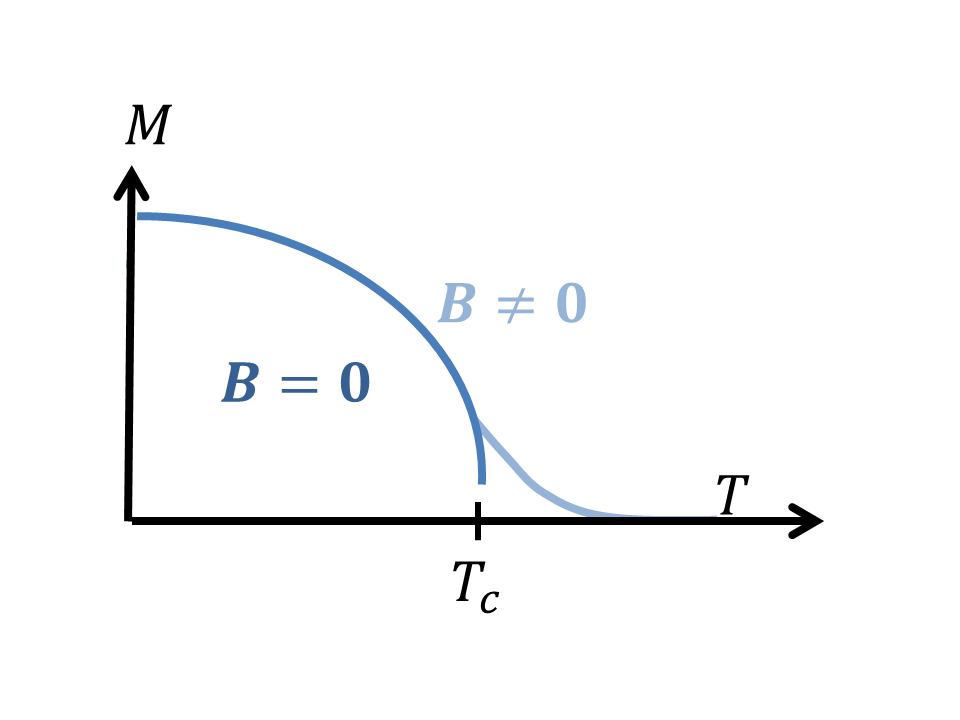
\includegraphics[width=\textwidth]{Folie42.png}
		\caption{Anschaulich zum Beispiel}
		\label{fig:Anschaulich}
		\centering
	\end{subfigure}
	\caption{} % \label{crossover}
\end{figure}	

\item \textbf{Crossover-Verhalten} \\
Skalenverhalten der freien Energie (siehe auch Abbildung \ref{crossover}) :
\begin{align}
G(B,\epsilon) \; =& \;  \vert \epsilon \vert ^\frac{1}{x_2} \; f^\pm \left( \frac{B}{\vert \epsilon \vert ^\frac{x_1}{x_2}} \right) \\
G(B,\epsilon) \; =  & \; \vert B \vert ^\frac{1}{x_1}\;  \; g \left( \frac{\epsilon}{B ^\frac{x_2}{x_2}} \right) \quad \quad \quad (B>0) \\
\end{align}
\begin{align}
\Rightarrow & B=0: \quad  G(0,\epsilon) \propto \vert \epsilon \vert ^\frac{1}{x_2} \propto \vert \epsilon \vert^{2- \alpha} \\
\Rightarrow & B \neq 0: \quad \mbox{solange } \frac{B}{\vert \epsilon \vert ^\frac{x_2}{x_1}} \ll 1 \quad \Leftrightarrow \quad B< \vert \epsilon \vert ^\frac{x_1}{x_2} \end{align}
Für $B\neq 0$ sieht man also ein gleiches kritisches Verhalten wie bei $ B=0.$ Erst wenn $ B/ \vert \epsilon \vert^\frac{x_1}{x_2} \approx 1 $ ändert sich das Verhalten.  $\to$ 'Crossover' zu anderem (oder keinem) kritischen Verhalten. Crossover setzt ein für $B \approx \vert \epsilon \vert^\frac{x_1}{x_2} = \vert \epsilon \vert ^{\Phi_B}$ \\
Für einen Ferromagnet im Feld beobachtet man jenseits des Crossover-Bereichs kein kritisches Verhalten. Es gibt aber erheblich interessantere Fälle, wo in Abhängigkeit von einem unsichtbaren %TODO wort stimmt?
 Systemparameter das kritische Verhalten wechselt (von einem zu einem anderen).
\end{itemize}

\subsection{Finite size scaling}
Phasenübergänge werden in einem endlichen System unterdrückt, weil $ \xi < L$. (Liniendimension %TODO wort?
des Systems). \\
Wir betrachten $\frac{1}{L}$ als Skalenfeld. (parameter, scaling field) \\
S-Ansatz: 
\begin{align}G(\xi, \frac{1}{L}) = \vert \epsilon \vert^{2-\alpha} \; f \left( \frac{\frac{1}{L}}{\vert \epsilon \vert^\Phi}\right) \; , \quad \quad \Phi = \mbox{ Crossover }
\end{align}
Wir erwarten, dass $G$ nur von dimensionslosen Größen abhängt:

\begin{align}
\frac{L}{\xi(T)} \quad \Rightarrow \quad \frac{\frac{1}{L}}{\frac{1}{\xi}} \; \propto \;  \frac{\frac{1}{L}}{\vert \epsilon \vert ^\nu} \quad \Rightarrow \quad \Phi = \nu
\end{align} Daraus folgt der allgemeine Ansatz:
\begin{align}
G(B, \epsilon, \frac{1}{L}) = \vert \epsilon \vert^{2-\alpha} \;  f^\pm \left( \frac{B}{\vert \epsilon \vert ^{\beta \delta}} ,\; \frac{1}{L \vert \epsilon \vert^\nu}\right) 
\end{align}
Betrachte: $\epsilon$ ist bezogen auf das unterschiedliche System $ \epsilon = \frac{T-T_c}{T_c}$ 
\begin{itemize}
\item[•] $L \gg \xi (T) \quad \Rightarrow \; L \vert \epsilon \vert ^\nu \gg  1,$ also verhält es sich wie ein unendliches System
\item[•] $ L \approx \xi (T) \quad \, \Rightarrow \; \vert \epsilon \vert \propto L^\frac{-1}{\nu}$ crossover 
\item[•]$L\ll \xi(T) \quad \Rightarrow \;$ Singularitäten verschwinden, kein Phasenübergang

\end{itemize}
\textbf{Beispiel:} ($B=0$, spezifische Wärme:) 
\begin{align*}
c \; \propto \;  \frac{\partial^2 G}{\partial \epsilon^2} \; \propto \; \vert \epsilon \vert^{-\alpha} \;  f^\pm \left( \frac{1}{L \vert \epsilon \vert^\nu}\right) 
\; \propto \;  L^\frac{\alpha}{\nu} (L^\frac{1}{\nu} \vert \epsilon \vert)^{-\alpha} \; f^\pm \left( \frac{1}{L \vert \epsilon \vert ^\nu }\right) 
\end{align*}
\begin{align*}
\Rightarrow \frac{c}{L^\frac{\alpha}{\nu}} = \tilde{f}^\pm \left( L^\frac{1}{\nu} \vert \epsilon \vert \right) = \tilde{f} \left( L^\frac{1}{\nu} \epsilon \right), \quad \mbox{ und } \quad c \propto L^\frac{\alpha}{\nu} \tag{bei $T_c$}
\end{align*} 
Andere Beispiele folgen in der Übung. 
Ohne Beweis gilt weiterhin: 
\begin{align*}
L^\frac{\beta}{\nu} M(\epsilon,L)=\underbrace{f}_{\substack{\text{ander-} \\ \text{es $f$}}}(L^\frac{1}{\nu} \epsilon) \quad \Rightarrow \quad M(0,L) \; = \; L^{-\frac{\beta}{\nu}} \; f(0)
\end{align*}
Siehe auch Abbildung \ref{fig:Anschaulich}. 
 \subsubsection*{Wie berechnet man $M(T)$ im System endlicher Größe?}
zu jedem Zustand $\mathbf{S}$ mit $M(\mathbf{S})$ gibt es einen (bei $ B=0$) gleichwahrscheinlichen Zustand $\mathbf{S}'= -\mathbf{S}$ mit $M(S') = - M(\mathbf{S})$. (Siehe auch nochmal Abbildung \ref{fig:Computer}.) \\
$\Rightarrow$ es ist 
\begin{align*}
M(T,B=0) \; = \;  \frac{1}{N} \sum_{i=1}^N \underbrace{\langle S_i \rangle}_{\substack{ \text{thermisches} \\ \text{ Mittel} \\ \widehat{=} \text{MC- Mittel}}} \; = \; 0 \quad \quad \quad \forall N
\end{align*} 
Der \textbf{Symmetriebruch} findet nur statt für: 

\begin{tcolorbox}[ams gather,title=, colback=blue!10!white, colframe=blue!30!black] 
\langle M(T,B=0) \rangle = \lim\limits_{B \to 0} \lim\limits_{N \to \infty} \langle M(T,B) \rangle 
\end{tcolorbox} 
Dies ist auch experimentell beobachtbar: endliche Systeme fluktuieren thermisch $(\pm M),$ sodass sie im Zeitmittel 'nicht-magnetisch' erscheinen $M \to 0$ \\
$\to$\textbf{Superparamagnetismus} \\ ($\Rightarrow$ Bedetung für Festplatten diskutieren!) \\

\textit{Zeitskala:} $\tau = \tau_0 e^\frac{\Delta E}{k_B T}$ \\
\textit{Energieverbrauch:} $\Delta E(L^n)$ (n meint Dimension: Oberfläche, Volumen...)\\ %TODO spinbild
$\Rightarrow$ zeitabhängiger (Algorithmus-abhängige) Ordungsparameterkurven. \\
Die Reihenfolge der Limites oben kann man nicht numerisch durchführen. Daher rechnet man: \\
 \begin{align}
  M(T,B=0) \; = \; \sqrt{\langle \left( \frac{1}{N} \sum_{i=1}^N S_i \right)^2 \rangle} = \sqrt{\langle S^2 \rangle} \label{EinfachereFormel}
\end{align} 
Mit (\ref{EinfachereFormel}) wird dann die Finite-Size-Scaling Analyse durchgeführt. 
\begin{itemize}
\item[•] innere Energie: \begin{align*}
U= \langle H \rangle
\end{align*}  
\item[•] spezifische Wärme:
\begin{align*}
 c_v= \frac{\partial U}{\partial T} \bigr\vert _{V,N}\; =\frac{1}{k_B T^2} \left( \langle H ^2 \rangle - \langle H \rangle^2 \right) 
\end{align*}
\item[•] Binder-Kummulante (4$^{th}$ order cummulant) zur Bestimmung von $T_c:$ 
\begin{align*}
U_L = 1-  \frac{\langle S^4 \rangle}{3 \langle S^2 \rangle^2}
\end{align*}
 mit folgenden Eigenschaften:
\begin{enumerate}
\item $T > T_c , \; L \gg \xi:  \quad \; U_L \to 0 \approx L^{- \alpha}$
\item $ T< T_c,  \; L \gg \xi: \quad \; U_L \to \frac{2}{3}$
\item $L \ll \xi: \quad   \quad  \quad  \quad \quad U_L \to U^* \; (L, T$ unabhängiger Zahlenwert)
\end{enumerate}
\end{itemize}

\begin{figure}[h] 
		\begin{subfigure}[h]{0.5 \textwidth}
		\centering
		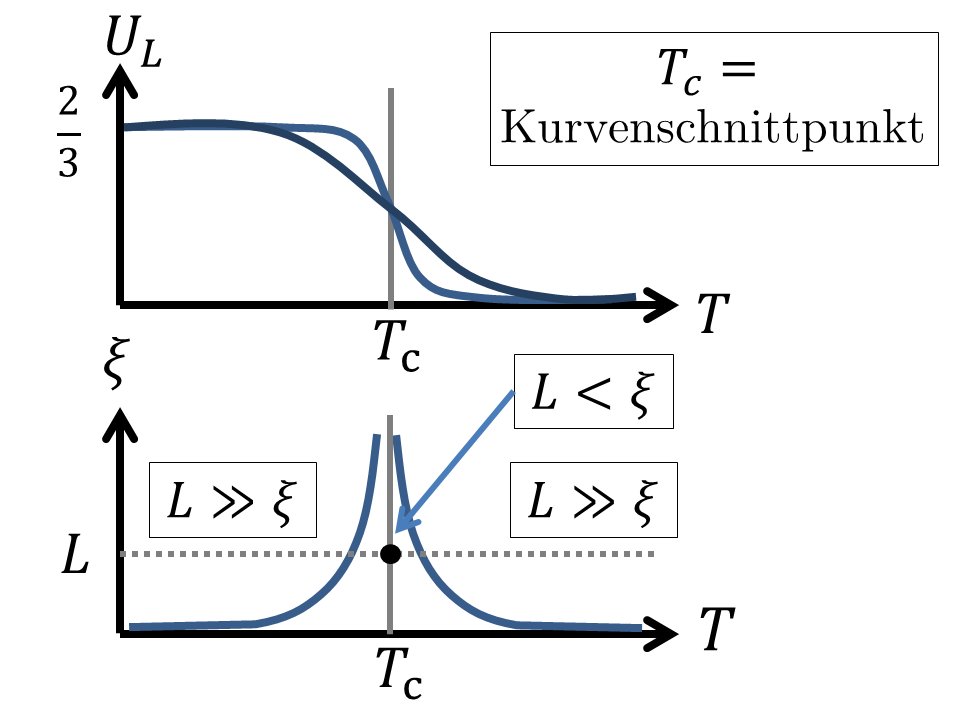
\includegraphics[width=\textwidth]{Folie43.png}
		\caption{Binder-Kummulante $U_L$ und $\zeta$} 
		\label{fig:Binder_Kummulante}
		\centering
	\end{subfigure}
	~
\begin{subfigure}[h]{0.5\textwidth}
		\centering
		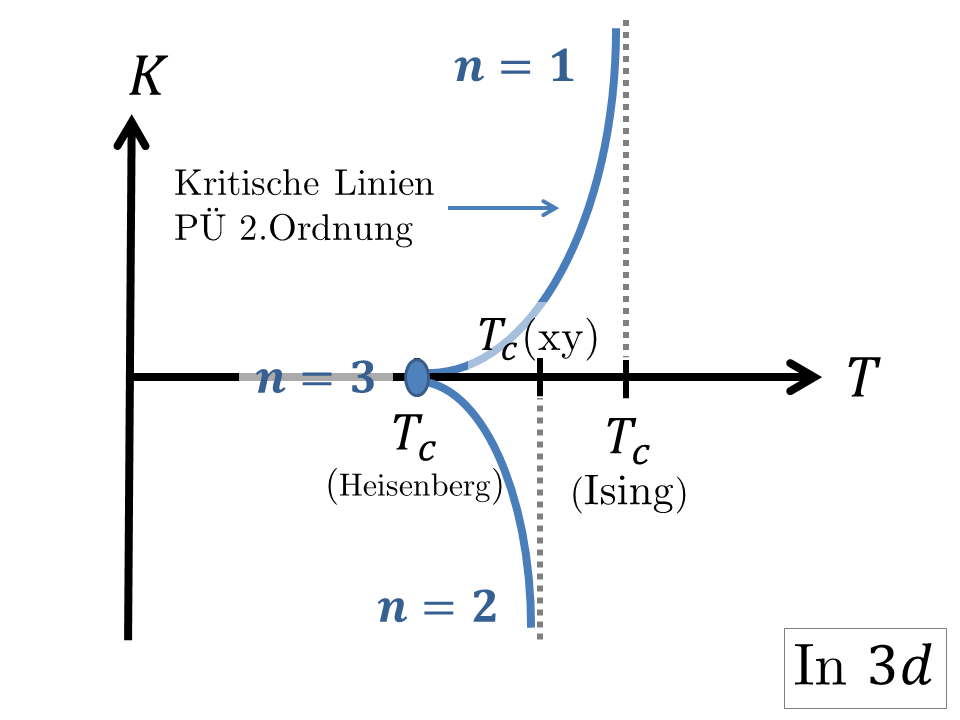
\includegraphics[width=\textwidth]{Folie44.png}
		\caption{Phasendiagramm}
		\label{fig:Phasen_Diagramm}
		\centering
	\end{subfigure}
	\caption{} % \label{crossover}
\end{figure}	

Siehe auch Abbildung \ref{fig:Binder_Kummulante}.
 \subsection{Kontinuierliche Freiheitsgrade: 'x-y' und Heisenbergs-Modell} \label{Kapitel2.9}
 Bislang betrachten wir \textsc{Ising}-Spins mit $ \uparrow \Rightarrow \downarrow$. Versuchs... %TODO word
 des Monte-Carlo-Algorithmus 'offensichtlich'. Wir betrachten jetzt (als Beispiel) Spinmodelle mit kontinuierlichen Freiheitsgraden.\\ 
 $3d$ Heisenberg-Ferromagnet mit axialer Anisotropie: 
 \begin{align}
 H= - J \sum_{i,j} \mathbf{S}_i \mathbf{S}_j - K \sum_i S_{iz}^2 \; , \quad \quad  \vert \mathbf{S} \vert
 =1
 \end{align}
 \textbf{Universalität:} Das kritische Verhalten hängt nicht von $J$ ab, sondern von Dimensionen des Ordnungsparameters!
 \begin{enumerate}
 \item $K= 0:  \quad$ $\mathbf{S}_i \cdot \mathbf{S}_j$ isotrop $ \quad \Rightarrow  \quad$ OP hat $n=3$ Komponenten $(m_x, m_y, m_z)$
 \item $K<0:  \quad$ Spins legen sich in $xy-$Ebene $ \quad \Rightarrow  \quad$ OP hat $2$ Komponenten ($m_x, \; m_y$)
 \item $K>0 : \quad$ Spins entlang $z-$Achse $ \quad \Rightarrow  \quad$ OP hat 1 Komponente ($m_z$)
 \end{enumerate}
 Das Phasendiagramm hierfür ist noch einmal in Abbildung \ref{fig:Phasen_Diagramm} ersichtlich.
 \begin{itemize}
 \item entlang der ($K=0$)-Linie anderes kritisches Verhalten (andere Exponenten) als für $K\neq 0$.
 \item für jedes endliche $K$ ist man im Universalitätsklasse von \textsc{Ising}- oder 'x-y'-Modell. 
 \item $K=0$: Heisenberg
 
 %TODO Tabelle von Gebhardt und krey als image
 \item besonders interessant: $2d-xy-Modell$ zeigt keine langreichweitige, ferromagnetische Ordnung aber einen \textsc{Kosterlitz-Thouless}-Übergang. ($\to$ Nobelpreis 2016) 
\end{itemize}
\subsection{MC-Algorithmen für kontinuierliche Freiheitsgrade}
\subsubsection{x-y-Modell}
\begin{figure}[h] 
		\begin{subfigure}[h]{0.5 \textwidth}
		\centering
		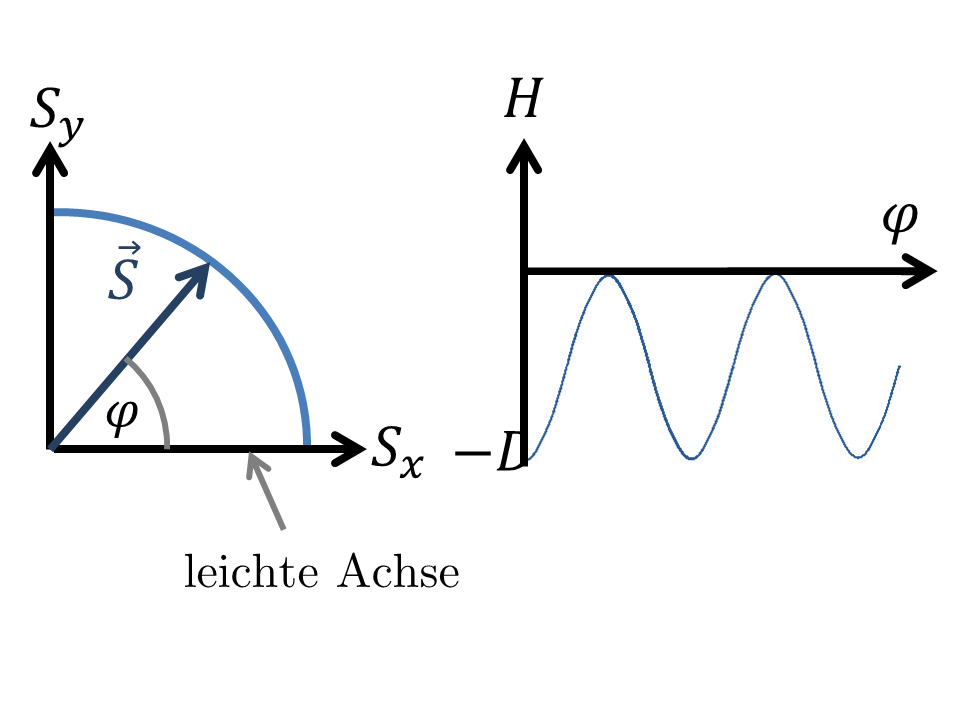
\includegraphics[width=\textwidth]{Folie45.png}
		\caption{\textbf{(oben)} kontinuierlicher Spin (magn. Moment)   im $1$-dimensionalen Potential \textbf{(unten)}} 
		\label{fig:Spin_Potential}
		\centering
	\end{subfigure}
	~
\begin{subfigure}[h]{0.5\textwidth}
		\centering
		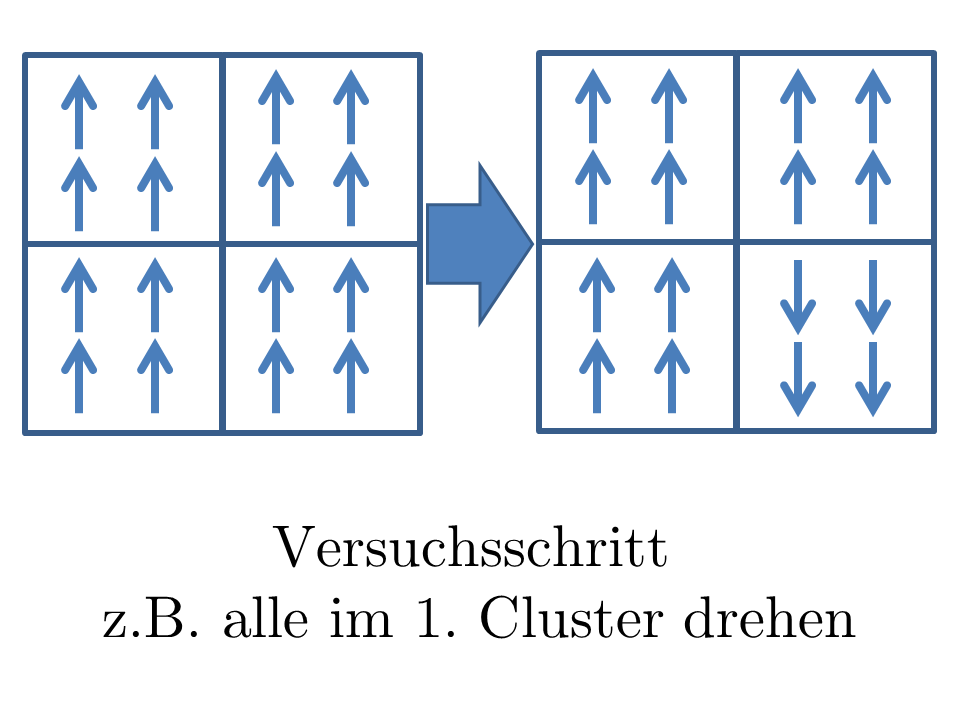
\includegraphics[width=\textwidth]{Folie46.png}
		\caption{Cluster-Algorithmus im \textsc{Ising}-Modell}
		\label{fig:Cluster_Ising}
		\centering
	\end{subfigure}
	\caption{} % \label{crossover}
\end{figure}	


Wir beachten kontinuierlichen 'Spin' (eigentlich ein magnetisches Moment) in der Ebene: $\vert \mathbf{S} \vert = 1$. Ein Spin davon mit Anisotropie \begin{align*}
H=-D \; S_x^2 = -D \cos(\phi)^2
\end{align*} mit dem Potential
\begin{align*}
V(x) = -D \cos(x)^2
\end{align*}
wie gezeigt in Abbildung \ref{fig:Spin_Potential}.

\textbf{Frage:} Wie wählt man den Versuchsschritt des Monte-Carlo-Algorithmus?
\begin{enumerate}

\item \textbf{Idee:} (Falsch!)
\begin{align*}
\varphi_{trial} = \varphi_{initial} \pm \Delta \varphi \quad \quad \quad \Delta \varphi = const.
\end{align*}
Falsch! Setze $\Delta \varphi = \pi$ \\
$ \Rightarrow$ anderes Modell (\textsc{Ising} $S_x = \pm 1$). Allgemein gilt, dass der MC-Algorithmus \textbf{ergodisch} sein muss, d.h. er muss genau den Phasenraum erreichen können!\footnote{genauer: Ergodisch bedeutet 'Zeit-Mittelwert $\widehat{=}$ Ensemble-Mittelwert'} \\
Ein anderes Beispiel für 'nicht-ergodisch' ist: \\
\textbf{Beispiel} ('naiver Clusteralgorithmus', Abb. \ref{fig:Cluster_Ising}) \\
Im \textsc{Ising}-Modell: bestimmte Konfigurationen können nicht vermischt werden. Trotzdem gibt es richtige (=also ergodische) und zudem sehr effektive Cluster-Algorithmen, wie beispielsweise \textit{Swendsten-Wang}. Da werden (immer andere) Cluster nach Regeln getrennt. 

\begin{figure}[h] 
		\begin{subfigure}[h]{0.5 \textwidth}
		\centering
		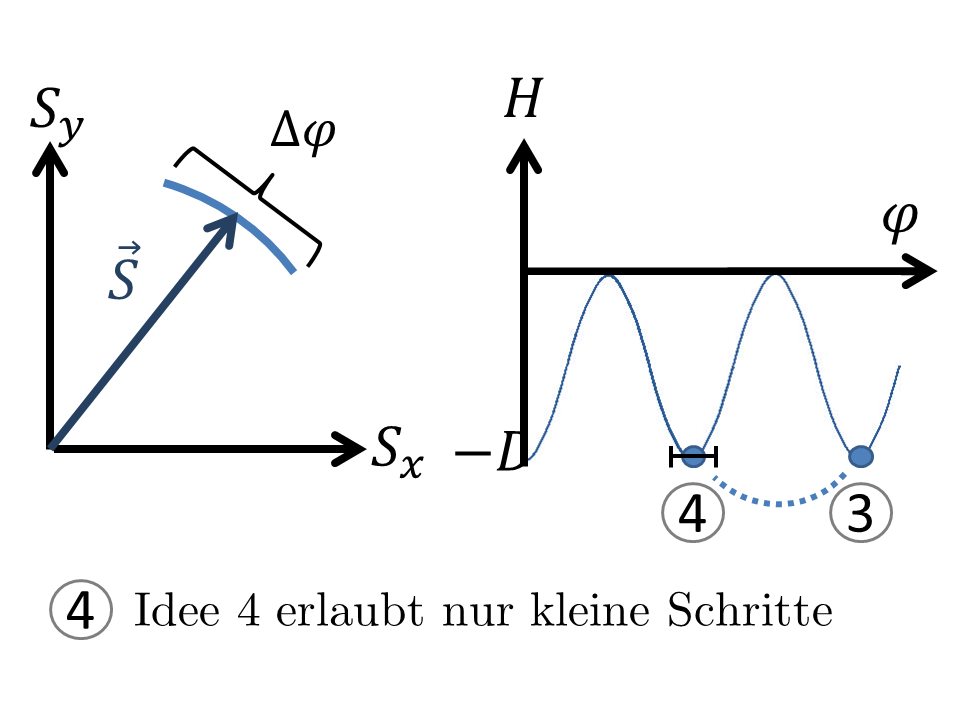
\includegraphics[width=\textwidth]{Folie47.png}
		\caption{Zufälliger Punkt auf Einheitskreis wird normiert. Nebendran werden Idee 3 und Idee 4 verglichen.} 
		\label{fig:zufaellig}
		\centering
	\end{subfigure}
	~
\begin{subfigure}[h]{0.5\textwidth}
		\centering
		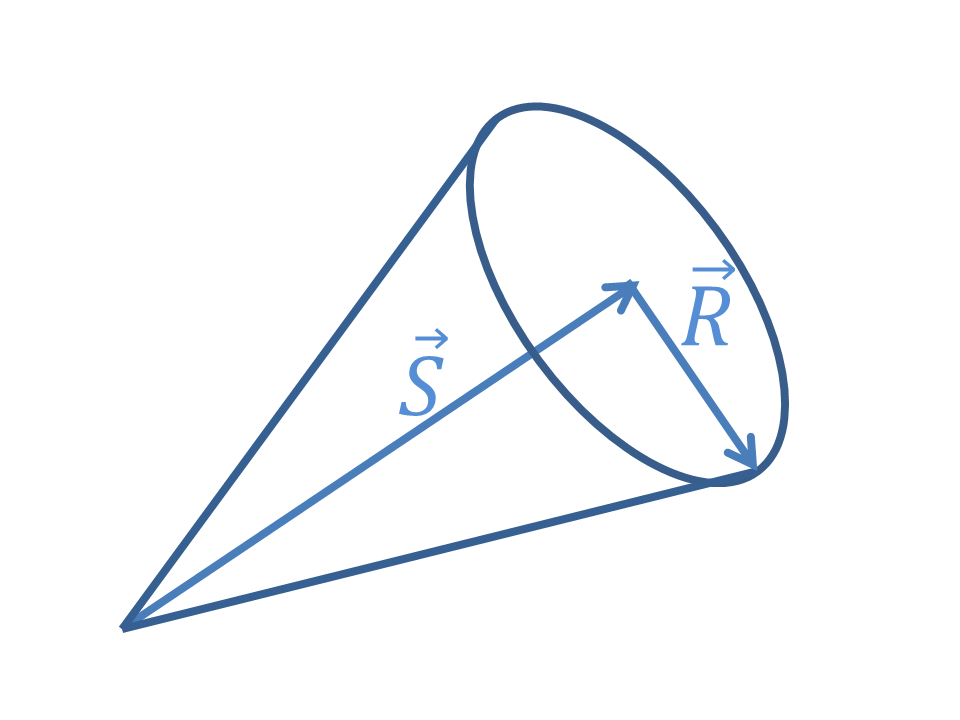
\includegraphics[width=\textwidth]{Folie48.png}
		\caption{Kleine Schritte um alten Vektor $\mathbf{S}$, hier: innerhalb eines Kegels}
		\label{fig:Kegel}
		\centering
	\end{subfigure}
	\caption{} % \label{crossover}
\end{figure}	


\item \textbf{Idee:} (falsch!) Wähle zufälligen Punkt im Einheitsquadrat und normiere. (Abb. \ref{fig:zufaellig})
Dieser ist auch falsch: Punkte auf dem Einheitskreis sind \textit{nicht} gleichverteilt, entlang Diagonale wahrscheinlicher
\begin{align*}
\frac{w(1 \to 2)}{w(2\to 1)} \overset{!}{=} e^{- \beta \; (E_2 - E_1)} = \frac{w_{t} (1 \to 2) \; w_{a} (1 \to 2)}{w_{t} (2 \to 1) \; w_{a} (2 \to 1) }  = \frac{w_t(2 \to 1)}{w_t(1 \to 2)} \; e^{-\beta \; (E_2-E_1)}
\end{align*}
\begin{align*}
\text{wobei} \begin{cases}
w_t: & \text{ Wahrscheinlichkeit, Wert vorzuschlagen} \\
w_a: & \text{Wahrscheinlichkeit zu akzeptieren}
\end{cases}
\end{align*}
sodass \begin{align*}
\Rightarrow \; w_t(2\to 1) = w_t(1 \to 2)
\end{align*}
\textbf{Allgemeine Symmetriebedingung:} Wahrscheinlichkeit für Versuchsschritte von Zustand $1 \to 2$ und zurück müssen gleich sein!

\item \textbf{Idee:}\label{Idee3} (stimmt!) Gleichverteilt auf Einheitskreis,\\ \textbf{z.B} $\varphi_i \in [0, 2\pi)$ gleichverteilt, $\Delta H = -D \cos (\varphi_{trial})^2 + D \cos (\varphi_{initial})^2$. \\
Und damit ergodisch und symmetrisch.

\item \textbf{Idee:}\label{Idee4} kleine Schritte um $\varphi_{initial}$: 
\begin{align*}
\varphi_{trial} = \varphi_{initial} + \delta_{trial} \quad \quad \quad \delta_{trial} \in [ - \Delta \varphi, \Delta \varphi ] \; \textit{(gleichverteilt)}
\end{align*}
Auch ergodisch und symmetrisch, wenn $\delta_{trial}$ symmetrisch gewählt wird.
\end{enumerate}

Idee \ref{Idee3} ist identisch mit Idee \ref{Idee4} für $\Delta \varphi = \pi$. Für kleines $\Delta \varphi \ll \pi$: Unterschiedliche Dynamik, wie gezeigt in Abbildung \ref{fig:zufaellig}. Allgemein muss Idee \ref{Idee4} über den Energieberg, um Spin umzudrehen, Idee \ref{Idee3} nicht. Daher sind die Relaxationszeiten verschieden, aber Gleichgewichtseigenschaften sind gleich. 




\subsubsection{Heisenberg-Modell}
\begin{align}
H= - \underbrace{\frac{J}{2} \sum_{i,j} \mathbf{S}_i \mathbf{S}_j}_{\substack{\text{Austausch} \\ \text{Nächste Nachbarn}}}
 - \underbrace{ D \sum_i S_{iz}^2}_\text{Anisotropie} - \underbrace{\mathbf{B} \sum_i \mathbf{S}_i}_\text{Magnetfeld} \; , \quad \quad \quad \vert \mathbf{S}_i \vert =1
\end{align}

\textbf{single spin flip Algorithmus:} Phasenraum des einzelnen Spins ist Einheitskugeloberfläche 
Der Versuchsschritt muss
\begin{itemize}
\item ergodisch
\item symmetrisch
\end{itemize} %TODO image
sein. 

\begin{enumerate}
		\item \textbf{gleichverteilt auf Einheitskugel} \\
		Wie erzeugt man Zufallsvariablen auf Einheitskugel?

\begin{itemize}
\item \textbf{rejection Methode:}
			
			\begin{itemize}
						\item  ziehe 3 Zufallszahlen $\in [ -1:1]$. $(z_x, 		z_y, z_z)$. 
						\item verwirf die Wahl, wenn außerhalb der Einheitskugel. $\sqrt{z_x^2 + z_y^2 +z_z^2}>1$.
						\item sonst normieren: 
\begin{align}
\begin{pmatrix} S_x^+ \\ S_y^+ \\ S_z ^+\end{pmatrix} = \begin{pmatrix} Z_x \\ Z_y \\ Z_z \end{pmatrix} \; \frac{1}{\sqrt{Z_x^2 + Z_y^2 + Z_z^2}}
\end{align}
						\item Schnelle Methode, beruht auf 3 Zufallszahlen und Algebra. Relative Zahl der berücksichtigten Tripel
\begin{align*}
\frac{\frac{4}{3} \pi (1)^3}{(2+1)^3} = \frac{\pi }{6}
\end{align*}
\end{itemize}		
		
			\item \textbf{Kugelkoordinaten} Flächenelement:
			Einheitsvektoren beschreiben Punkte auf der Einheitskugeloberfläche. Flächenelement in Kugelkoordinaten ist:
			\begin{align}
			dF= \underbrace{r^2}_\text{=1} sin(\Theta) \; d \Theta d\varphi
			\end{align}	
			Würde man gleichverteilte Zufallszahlen in $\Theta$ und $\varphi$ nehmen, wären die Vektoren auf der Einehitskugeloberfläche nicht gleichverteilt, da $dF \propto sin(\Theta)$ \\
			\textit{Aber:} 
			\begin{align*}
			sin(\Theta) \; d\Theta = - d \, cos(\Theta) = -dz \quad \quad \quad S_z =cos(\Theta)
			\end{align*}
			das heißt 
			\begin{align*}
			\Rightarrow dF= - d S_z \; d \phi 
			\end{align*}
			$ \Rightarrow$man kann $S_z$ und $\phi$ gleichverteilt aus $[-1:1]$ und $[0:2\pi)$ wählen. \\
			$\Rightarrow$ Dies erzeugt gleichverteilte Vektoren auf der Einheitskugeloberfläche mit
\begin{align*}
 \begin{pmatrix} S_x \\ S_y \\ S_z \end{pmatrix} =  \begin{pmatrix} \sqrt{1-S_z^2} \; \cos(\varphi) \\ \sqrt{1-S_z^2} \; \sin(\varphi) \\ S_z \end{pmatrix}
\end{align*}
			\\ 
\textbf{Nachteil:} $\cos(),\sin()$ müssen gerechnet werden $\to$ langsam!			
\end{itemize}
			
			
			\item \textbf{ kleine Schritte um den alten Vektor $\mathbf{S}$ innerhalb eines Kegels}, wie in Abbildung \ref{fig:Kegel} gezeigt:
			\begin{itemize}
			\item[-] erzeuge Zufallsvektor $\mathbf{S}_r$ innerhalb einer Kugel, also mit maximalen Radius R.
			\item[-] rechne 
			\begin{align}
			\mathbf{S}_r = \frac{\mathbf{S} + \mathbf{S}_r}{\sqrt{\mathbf{S}^2 + \mathbf{S}_r^2}}
			\end{align} d.h. addiere $\mathbf{S}_r$ und normiere.
			\item[-] $\mathbf{S}_r$ aus rejection Methode ohne Normierung
			\end{itemize}
			
			
Diese Methode erzeugt kleine Schritte (je nach Wahl von $R$), sodass Anisotropie-Energiebarrieren überwunden werden müssen $\to$ Konsequenzen für die Dynamik.  \\
Man kann maximale Schrittweite $R$ berechnen um einen Monte Carlo Schritt zu eichen, also auf ein 'echtes' Zeitintervall im %TODO word 
der dissipativen Dynamik des Systems abzubilden $\to$ Zeitquantifizierung \textit{('time quantified Monte Carlo')}		
\end{enumerate}


 \subsection{Perkolation}
 	\begin{itemize}
 	\item betrachte Gitter in d Dimensionen\footnote{$(1d, \; 2d, \; 3d)$}
 	\item besetze Plätze (Verbindungen) mit Wahrscheinlichkeit $p$
 	\item definiere Nachbarschaft, z.B via nächste Nachbarn\footnote{je nach Fall vielleicht auch übernächste Nachbarn... bei Dottierung einer Monolage beispielsweise}
 	\item Perkolation beschäftigt sich mit Clustern, d.h.  besetzter, benachbarter Gitterplätze %TODO image cluster
 	\item speziell oberhalb der sogenannten \textbf{Perkolationswahrscheinlichkeit} (oder Perkolationsgrenze) $p_c$ gibt es einen $\infty$ großen, perkolierenden Cluster. \footnote{$2d: \; \infty $ große Cluster  nicht möglich, in $2d$ schon.}
 	$\Rightarrow$ wichtig für z.B. Leitfähigkeit, (ferro)magnetische Ordnung 
 	\begin{center}
 	
 	
 	\begin{tabular}{c||c c c}
 	%\hline 
 	 &  & $\mathbf{p_c}$ &\textbf{ bond} \\ 
 	\hline 
 	\textbf{2d} & Quadrat & 0.592 & 0.5 \\ 
 	%\hline 
 	 & sc & 0.312 & 0.249 \\ 
 	%\hline 
 	\textbf{3d} & fcc & 0.198 & 0.119 \\ 
 	%\hline 
 	 & bcc & 0.245 & 0.179 \\ 
 	%\hline 
 	\end{tabular} \\
 	\end{center} 
 	\end{itemize}
 	\textbf{Definition Korrelationsfunktion:}\\
 	
 	\begin{figure}[ht]
\centering
\includegraphics[width=0.45\textwidth]{Folie49.png}
	\caption{}
	\label{fig:Korrelationsfunktion}
\end{figure}

 	 $g( \vert \mathbf{r}_1 - \mathbf{r}_2 \vert)$: Wahrscheinlichkeit, dass $\mathbf{r}_1$ und $\mathbf{r}_2$ zum gleichen Cluster (Abb. \ref{fig:Korrelationsfunktion}) gehören. \\
 	\textbf{Korrelationslänge:}
 	 \begin{align}
 	\xi^2= \frac{\sum_r r^2 g(r)}{\sum_r g(r)}
 	\end{align}
 	diese Definition ist vereinbar mit $g(r) \propto e^\frac{-r}{\xi}$, da 
 	\begin{align}
 	\frac{\int d^3r \; r^2 \; e^\frac{-r}{\xi}}{\int d^3 r \; e^\frac{-r}{\xi}}
 	= \frac{\int_0^\infty dr \; r^4 \; e^\frac{-r}{\xi}}{\int_0^\infty d r \; r^2 \; e^\frac{-r}{\xi}}
 	= \frac{\xi^5}{\xi^3}  \frac{\int d^3r \; r^2 \; e^\frac{-r}{\xi}}{\int d^3\;  r \; e^\frac{-r}{\xi}} \; \propto \; \xi^2
 	\end{align}
 	
 	\begin{itemize}
 	\item $p>p_c: \quad$Beitrag des $\infty$-großen Clustern wird subtrahiert \\ $\Rightarrow \; g(r)$ geht immer gegen Null
 	\item $p \to p_c: \quad $ $\xi(p) \propto \vert p-p_c \vert^{-\nu}$ mit kritischem Exponenten $\nu$. Wieder gilt die Universalität $\nu_{2d} = \frac{4}{3}, \; \nu_{3d} = 0,88$ unabhängig vom Gitter!
 	
 	\end{itemize}

 	 	Wir betrachten die Wahrscheinlichkeitsvertielung $D(s,p)$ für Cluster der Größe $s$: 
\begin{align}
 	D(s,p)=& (1-p)^2 \; p^s
 	= (1-p)^2 \; e^{ln(p)s} = (1-p)^2 \underbrace{e^{- \vert ln(p) \vert s}}_\text{Korrelationslänge} = (1-p)^2 e^{-\frac{s}{\xi}}
\end{align}

 	mit Korrelationslänge
 	\begin{align*}
 	\xi = \frac{1}{\vert ln(p) \vert} = -\frac{1}{ln(p)}, \quad \quad \quad ln(p)= p-1= p-p_c \quad \mbox{ wobei } p_c=1
\end{align*}
Wir entwickeln um $p-p_c$: \begin{align*}
ln(p) \approx p-1  \quad \quad \Rightarrow \quad \quad  \xi (p \to p_c) = \frac{1}{p_c-p}= (p_c - p)^\nu 
\end{align*}
 	mit dem kritischen Exponenten $\nu =1$ der Korrelationslänge. \\
 	
 	In höheren Dimensionen $D>1$ sind nur numerische Verfahren möglich. Zentrale Größe für die Analyse ist die Verteilungsfunktion der Clustergrößen $D(s,p)$.
 	\subsubsection{nummerisches Verfahren zur Clusteranalyse}
 	
 	 		\begin{enumerate}
 		\item Rekursiv (Abb. \ref{fig:hello})
 		\begin{figure}[ht]
\centering
\includegraphics[width=\textwidth]{hello.png}
	\caption{}
	\label{fig:hello}
\end{figure}
 		
 			\begin{itemize}
 			\item Schleife durch das Gitter
 			\item 1.Besetzter Platz erhält Index 1
 			\item Nachbarn werden besucht, falls besetzt nicht indiziert
 			\item weiter zum nächsten Platz falls besetzt und falls nicht indiziert, dann Index 2...
 			\end{itemize}
 			
 		\item schneller: \textbf{Hoshen-Kopelmann-Algorithmus}
 		
\end{enumerate} 	

Die \textbf{Cluster-Analyse} erlaubt weitere Auswirkung der Verteilungsfunktionen $D(s,p)$.
\begin{itemize}
\item in der Nähe des kritischen Punktes $p_c$ gilt $D(s,p_c) \propto s^{-\epsilon}$ mit einem kritischen Exponenten $\epsilon$.
\item weiter weg gilt $D(s,p) \propto e^{-\frac{s}{\xi}}$ mit $\xi (p) \propto \vert p_c - p \vert ^{- \nu}$
\item das perkulierende Cluster am kritischen Punkt ist ein Fraktal
\end{itemize}	 
\textbf{Fraktal:} 
\begin{itemize}
	\item gebrochene Dimension \begin{align}
	s \propto \underbrace{r^{D_f}}_{\substack{\text{Gyrations-} \\ \text{radius}}} \mbox{ fraktale Dimension } D_f
\end{align}	 
\item 'normal' wäre Fläche $F \propto r^2$ und Volumen $V \propto r^3$. $D_f$ ist dabei kleiner als die einbettende Dimension $(2,3)$
\item Fraktale sind selbstähnlich\footnote{hier im statistischen Sinne}
\end{itemize}

\begin{figure}[h] 
		\begin{subfigure}[h]{0.5 \textwidth}
		\centering
		\includegraphics[width=\textwidth]{Folie55.png}
		%\caption{} 
		%\label{fig:Symmetriebruch}
		\centering
	\end{subfigure}
	~
\begin{subfigure}[h]{0.5\textwidth}
		\centering
		\includegraphics[width=\textwidth]{Folie56.png}
		%\caption{}
		%\label{fig:Computer}
		\centering
	\end{subfigure}
	\caption{ Fraktale} \label{Fraktale}
\end{figure}	

\textbf{Beispiel:} aus der Mathematik (Abb. \ref{Fraktale}):

allgemein: \begin{align*}
ln(as)= a^x ln(s) \quad \quad \quad   4=3^x \Rightarrow x= \frac{ln(4)}{ln(3)}
\end{align*}


setze:\begin{align*}
a= \frac{1}{s} \quad \Rightarrow \quad ln(1)= \left( \frac{1}{s} \right)^x ln(s) \quad \Rightarrow \quad ln(s)= ln(1) s^x
\end{align*} 
$x$ bezeichnet man dabei als die fraktale dimension.

\section{Molekulardynamiksimulationen}
Es gibt 2 Klassen von Verfahren in der statistischen Physik: 
\begin{enumerate}
\item Monte Carlo (kanonische Gesamtheit)
\item Molekulardynamik (zunächst) mikrokanonisch, d.h. die Energie bleibt erhalten. Durch Lösen der Bewegungsgleichungen für viele Teilchen \\
\end{enumerate}
$\Rightarrow$ Wir brauchen ein Verfahren zur nummerischen Lösung von DGL \\
\textbf{Dynamische Systeme} 
ist beispeilsweise die Newtonsche Bewegungsgleichung 
\begin{align}
m \ddot{\mathbf{r}} = \mathbf{F} (\mathbf{r}, \dot{\mathbf{r}}, t) \quad \quad \quad \mathbf{r} \in \mathbb{R}^3 \; \text{(pro Teilchen)}
\end{align} mit der Bahn $\mathbf{r}(t)$. Hier haben wir 3 DGLn $2.$Ordnung mit den zwei Anfangsbedingungen
\begin{align*}
r(t=0) \quad \quad  \quad \quad \dot{r}(t=0)
\end{align*}
Wir führen neue Variablen ein 
\begin{align*}
\begin{cases}
\dot{\mathbf{r}}= \mathbf{v} \\
\dot{\mathbf{v}} = \frac{1}{m} \mathbf{F}(\mathbf{r}, \mathbf{v},t) 
\end{cases}
\text{ mit }
\begin{pmatrix}\mathbf{r}\\ \mathbf{v}\end{pmatrix} \in \mathbb{R}^6
\end{align*}
Es handelt sich um 6 DGLn 1.Ordnung (siehe auch 'Hamilton Formalismus') %TODO verlinken?
. Es genügt aber eine DGL folgenden Typs zu studieren: 
\begin{align}
\dot{\mathbf{x}}= \mathbf{f}( \mathbf{x},t) \quad \quad \quad \quad \mbox{  mit  } x \in \mathbb{R}^n \tag{\textbf{Dynamisches System}}
\end{align}

\subsection{ \textsc{Euler} Verfahren}
Eindimensional $\dot{x}= f(x,t)$, Abb. \ref{fig:Euler}.\\  

\begin{figure}[ht]
\centering
\includegraphics[width=0.7\textwidth]{Folie57.png}
	\caption{}
	\label{fig:Euler}
\end{figure}
 
\textbf{Taylor:}
\begin{align}
x(t_0 +h)=& x(t_0) + \dot{x}(t_0)h+ \mathcal{O} (h^2) \\
=& x(t_0) + f(x,t_0) h+ \mathcal{O} (h^2)
\end{align}
\textbf{Diskretisierung der Zeit:}
\begin{align*}
\begin{rcases}
t_n = t_0 + nh \\ 
x_n = x(t_n)
\end{rcases}
\quad \quad \quad n=0,1,2,...
\end{align*}
\textbf{Euler:}
\begin{tcolorbox}[ams gather,title=, colback=blue!10!white, colframe=blue!30!black] 
 x_{n+1}= x_n + f(x_n, t_n)h+ \mathcal{O}(h^2)
\end{tcolorbox}
Fehler des Einzelschritts $\propto h^2$. Für ein Intervall der Länge $T$ benötigt man $N= \frac{T}{h}$ Schritte.
\begin{tcolorbox}[ams gather,title=, colback=blue!10!white, colframe=blue!30!black] \text{Gesamtfehler} \propto h^2 N \propto h 
\end{tcolorbox}
Fehler oben heißt \textbf{systematischer Fehler}. Er entsteht durch die Approximation. Verkleinern durch $h \to 0$ - Geht das? Nein! Wegen \textit{Rundungsfehlern} und eventueller \textit{Instabilitäten}.


\subsection{Stabilitätsanalyse}
$x_n$: berechne Werte $x(t)$ mit Fehler $\epsilon_n$:

\begin{align}
\mathbf{x}_{n+1} + \boldsymbol{\epsilon}_{n+1} =\mathbf{x}_n + \boldsymbol{\epsilon}_n + \mathbf{f}( x_n + \boldsymbol{\epsilon}_n, t_n) \Delta t := \mathbf{T}(\mathbf{x}_n + \boldsymbol{\epsilon}_n)
\end{align} 

 entwickle $T$ für kleines $\boldsymbol{\epsilon}_n$: 
 \begin{align}
 \mathbf{T}(\mathbf{x}_n + \boldsymbol{\epsilon}_n) 
 \approx \mathbf{T}(\mathbf{x}_n) + \underbrace{\frac{d\mathbf{T}}{d\mathbf{x}}}_{ \substack{ \text{Funktional-} \\ \text{matrix} \\  \text{ (Jacobi)} }} \biggr\vert_{x_n} \cdot \boldsymbol{\epsilon}_n \quad
 \Rightarrow \quad \epsilon_{n+1} = \frac{d\mathbf{T}}{d\mathbf{x}}  \biggr\vert_{x_n} \boldsymbol{ \epsilon}_n  \equiv \underline{ \underline{\mathbf{G} }} \;  \boldsymbol{\epsilon}_n \; 
 \end{align}
 weil
 \begin{align*}
 \mathbf{x}_{n+1} = \mathbf{T}_{x_n}
 \end{align*}
 
Der Fehler divergiert nur dann nicht, wenn für alle Eigenwerte von $\underline{ \underline{\mathbf{G} }}$, $\vert g_i \vert \leq 1$ gilt\footnote{Achtung, $g_i$ kann komplex sein!}.
\\
\textbf{Beispiel 1: }
\begin{align*}
\frac{dx}{dt}= - \lambda \; x \quad \quad \quad \text{  (zum Beispiel radioaktiver Zerfall für } \lambda > 0)
 \end{align*}
 \textit{Euler:}
 \begin{align*}
 x_{n+1} = \;  x_n ( 1- \lambda \Delta t) = T (x_n) \quad
 \Rightarrow \quad \epsilon_{n+1} = \frac{dT}{dx} \biggr\vert _{x_n} \epsilon_n \; =\;  (1- \lambda \Delta t) \; \epsilon_n 
 \end{align*}
 \begin{align}
   \Rightarrow  \vert 1 - \lambda \Delta t \vert <1 , \quad \quad \quad \forall \lambda > 0, \Delta T \to 0
 \end{align}
$\Rightarrow$ stabil! (instabil für $\lambda < 0$) \\

\textbf{Beispiel 2:} (harmonischer Oszillator)
\begin{align}
\ddot{z}= - \omega^2 z &  
\end{align}
\begin{align*}
\begin{rcases}
x_1 = z \\
x_2 = \dot{z} &(v)
\end{rcases}
\; \Rightarrow \; 
\begin{rcases}
\dot{x}_1 = x_2  & (\dot{z}=v) \\
\dot{x}_2 = - \omega^2 x_1 & (\dot{v}= - \omega ^2 z)
\end{rcases}  
\;  \Rightarrow \; 
\begin{rcases}
x_1 (n+1) = x_1(n) + x_2 (n) \Delta t \\
x_2 (n+1) = x_2(n) - \omega^2 x_1 (n) \Delta t
\end{rcases} 
\end{align*}
\begin{align}
\Rightarrow \underline{ \underline{\mathbf{G} }} = 
\begin{pmatrix}
 1 & \Delta t \\
 - \omega^2 \Delta t & 1
\end{pmatrix}
\end{align}
für Eigenwerte aus 
\begin{align}
\begin{vmatrix}
1-g & \Delta t \\
- \omega^2 \Delta t & 1-g
\end{vmatrix}
\overset{!}{=} 0 \quad \quad \Leftrightarrow \quad \quad 0=  (1-g)^2 + \omega^2 \Delta t^2 
\end{align}
\begin{align*}
\Leftrightarrow \quad  g_{1,2} = 1 \pm i\omega t \quad 
\Leftrightarrow  \quad \vert g_{1,2} \vert = \sqrt{1 + \omega^2 \Delta t^2} <1,\quad \forall \; \omega, \Delta t \quad \Rightarrow \quad  \mbox{immer instabil}
\end{align*}
Anschauliche Erklärung: Was passiert? \\
Wir betrachten noch einmal: 
 \begin{align}
\dot{x}= f(x) = - \lambda x \quad \quad \Rightarrow \quad \quad x(t) = x_0 e^{-\lambda t} \quad \quad \Rightarrow \quad \quad \text{stabil}
\end{align}

\begin{figure}[h] 
		\begin{subfigure}[h]{0.5 \textwidth}
		\centering
		\includegraphics[width=\textwidth]{Folie58.png}
		\caption{stabil} 
		%\label{fig:Symmetriebruch}
		\centering
	\end{subfigure}
	~
\begin{subfigure}[h]{0.5\textwidth}
		\centering
		\includegraphics[width=\textwidth]{Folie59.png}
		\caption{instabil}
		%\label{fig:Computer}
		\centering
	\end{subfigure}
	\caption{Anschauliche Erklärung} \label{Anschaulich}
\end{figure}	
%TODO image BEARBEITEN!!!

\begin{align*}
x_{n+1} \; = \; x_n + \Delta t \; f(x_n, t_n) \; = \; x_n - \lambda x_n \, \Delta t
\end{align*}
\begin{align*}
\dot{x} = f(x) = + \lambda x \quad \quad \Rightarrow \quad \quad \lambda > 0 \quad \quad \Rightarrow \quad \quad \text{instabil}
\end{align*}
Siehe Abbildung \ref{Anschaulich}. 
\paragraph{Weitere Tests (nummerisch):}
\begin{itemize}
\item Erhaltungssätze überprüfen: Energie-, Impuls-, Drehimpulserhaltung 
\item Rückwärtsintegration
\end{itemize}
\subsection{Runge-Kutta Verfahren}
Es gibt viele bessere Verfahren
\begin{itemize}
\item[-]stabiler
\item[-]schnellere Konvergenz
\end{itemize}

Warum schneller? Schneller muss dabei im einzelnen abgewogen werden: \\
 $\to$ 'CPU-Zeit $\Leftrightarrow$ bessere Konvergenz'.\\

\textit{Euler:} 

\begin{align*}
 x(t_n +h)  &= x(t_n) + \dot{x}(t_n) \cdot h + \mathcal{O}(h^2) \\
 x(t_n -h) &= x(t_n) - \dot{x}(t_n) \cdot h + \mathcal{O}(h^2)  
 \end{align*}
 \begin{align*}
 \Rightarrow \quad  x(t_n +h) - x(t_n -h) =\; 2 h\;  \dot{x}(t_n)  + \mathcal{O}(h^3)
\end{align*}
Lösung von $\dot{x}= f(x,t):$

%\begin{mymathbox}[ams gather, title=two equations, colframe=blue!30!black]
\begin{tcolorbox}[ams gather,title= Runge-Kutta 1. Stufe, colback=blue!10!white, colframe=blue!30!black] 
x_{n+1}= x_{n-1} + 2 h f(x_n, t) + \mathcal{O} (h^3)  \nonumber \\
x_{n+2}= x_{n} + 2 h f(x_{n+1}, t) + \mathcal{O} (h^3) 
\end{tcolorbox}
%TODO %TODO %TODO Schablone von boxes
Man nennt dies auch \textbf{'Bocksprung', 'Leap-Frog'} oder \textbf{'Merhschrittverfahren'}.\\ 


\begin{figure}[h] 
		\begin{subfigure}[h]{0.5 \textwidth}
		\centering
		\includegraphics[width=\textwidth]{Folie60.png}
		\caption{RK 1.Stufe, Prinzip} 
		\label{fig:RK1}
		\centering
	\end{subfigure}
	~
\begin{subfigure}[h]{0.5\textwidth}
		\centering
		\includegraphics[width=\textwidth]{Folie61.png}
		\caption{RK 2. Stufe im Vergleich mit Euler}
		\label{fig:RK2}
		\centering
	\end{subfigure}
	\caption{} 
\end{figure}	


\textbf{noch besser:} Runge-Kutta 2.Stufe.
\begin{align*}
x_{n+1} =& x_{n-1}+2hf(x_{n}, t_n) + \mathcal{O}(h^3) 
\end{align*}
man braucht wegen $x_{n-1}$ und $x_n$ zwei Anfangswerte. Berechne $x_n$ aus Euler:
\begin{align*}
x_n = &x_{n-1} + h f(x_{n-1}, t_{n-1}) + \mathcal{O}(h^2)  
\end{align*}
umschreiben mit
\begin{align*}
2h=\bar{h}
\end{align*}
liefert
%\begin{empheq}[box=\othermathbox]{align}
\begin{tcolorbox}[ams align, title= Runge-Kutta 2. Stufe, colback=blue!10!white, colframe=blue!30!black] 
K &=\frac{1}{2} \; \bar{h} \; f(x_n, t_n) \nonumber \\ 
x_{n+1} &= x_n + \bar{h} \; f(x_n+k, \;  t_n+ \frac{1}{2} \bar{h}) + \mathcal{O}(h^3) \\
t_{n+1} & = t_n \,+ \bar{h}  \nonumber
\end{tcolorbox}

Auch bekannt als \textbf{'Zwischenschritt-Verfahren'}. \\
%TODO image

\textbf{Beispiel:} (DGL 2. Ordnung)
\begin{align}
\ddot{x}= f(x,t) \qquad \Rightarrow \qquad \begin{cases}
\dot{x}=v \\
\dot{v}= f(x,v,t)
\end{cases}
\end{align}
\textit{RKZ:}\begin{align*}
K_x =&\; \frac{1}{2} \;  h \; v_n \\
K_v = & \; \frac{1}{2} \; h \; f(x_n, t) \\
x_{n+1} =&\; x_n +h \;  (v_n + K_v)  \\
v_{n+1}= &\; v_n + h \; f(x_n+K_x, \;  v_n+K_v, \;  t_n+\frac{1}{2}h)  \\
t_{n+1} =&\;  t_n + h
\end{align*}
\textbf{(ohne Beweis:) Runge Kutta 4.Stufe:}
\begin{align*}
K_1&= h\; f(x_n, \; t_n) \\
K_2&=h \; f(x_n + \frac{1}{2} K_1, \; t_n + \frac{h}{2}) \\
K_3&= h\;  f(x_n + \frac{1}{2} K_2, \; t_n + \frac{h}{2}) \\
K_4&= h\;  f(x_n +  K_3, \; t_n + h)  \\
x_{n+1}&= x_n + \frac{1}{6} (K_1 + 2 K_2 + 2 K_3 + K_4) + \mathcal{O}(h^5)\\
t_{n+t} &= t_n + h 
\end{align*}
Prinzip: 4 Punkte werden zur Integration herangezogen.
\begin{align*}
\dot{x}=& f(x,t) \qquad \Rightarrow \qquad  x_{n+1} - x_n = \int_{t_n}^{t_n+h} dt \; f(x(t), t) \qquad \quad x(t) \text{ aber unbekannt!}
\end{align*}

\subsection{Schrittweitenanpassung}
\begin{itemize}
\item einfachste Vorgehensweise: feste Schrittweite $h +$Tests, ob die Lösung wirklich stabil, richtig... ist.
\item unter Umständen ist aber eine dynamische Anpassung der Schrittweite besser. Anpassung durch Vergleich (z.B. von RK2 und RK4) \\
\end{itemize}

RK2: \begin{align}
x_{n+1} = x_n + K_2 + \mathcal{O}(h^3)
\end{align}
RK4: \begin{align}
x_{n+1} &= x_n + \frac{1}{6} (K_1 + 2K_2 +2K_3 + K_4) \\
&= x_n + K_2 + \underbrace{\frac{1}{6} (K_1 - 4K_2 + 2K_3 +K_4)}_\delta + \mathcal{O}(h^5)
\end{align}
$\delta$ ist ein Maß für den Fehler von RKZ und 
\begin{align*}
\delta = \mathcal{O}(h^3)
\end{align*} 
Wir definieren weiterhin den \textbf{relativen Fehler:} 
\begin{align}
\left| \frac{\delta}{K_2} \right| = \mathcal{O}(h^2)
\end{align}
und versuchen diesen Fehler konstant zu halten
\begin{align}
\left| \frac{\delta}{K_2} \right| = a\; h^2 \overset{!}{=} \epsilon.
\end{align}
Dieser wird vorgegeben durch Wahl von $h$. Verlange 
\begin{align}
a \;  h_{neu}= \epsilon \qquad \Rightarrow \qquad h^2 = \frac{\epsilon}{a} = h^2 \frac{\epsilon}{\left| \frac{\delta}{K_2} \right|} 
\end{align}
\begin{align}
\tcboxmath{ h_{neu} = h \sqrt{\frac{\epsilon}{\vert \frac{\delta}{K_2} \vert }}}
\end{align}
\textbf{also:} 
\begin{itemize}
\item[-] $h$ vorgegeben $
\to \epsilon = \left| \frac{\delta}{K_2} \right| $
\item[-] $\epsilon$ konstant halten 
\item[-] immer wieder neues $h$ berechnen aus $ \left| \frac{\delta}{K_2} \right|$
\end{itemize}

\subsection{Prädikator-Korrelator-Verfahren}

\begin{figure}[h] 
		\begin{subfigure}[h]{0.5 \textwidth}
		\centering
		\includegraphics[width=\textwidth]{Folie62.png}
		%\caption{} 
		%\label{fig:Symmetriebruch}
		\centering
	\end{subfigure}
	~
\begin{subfigure}[h]{0.5\textwidth}
		\centering
		\includegraphics[width=\textwidth]{Folie63.png}
		%\caption{}
		%\label{fig:Computer}
		\centering
	\end{subfigure}
	\caption{} \label{Praedikator}
\end{figure}	


Ein sehr genaues und stabiles Verfahren. Hier soll nur das Prinzip erläutert werden. (Siehe auch Abb. \ref{Praedikator})
\begin{align*}
\dot{x}= f(x,t) \qquad \overrightarrow{_{Integrieren}} \qquad x(t+h) = x(t) + \int_t^{t+h} dt' \; f(x(t'), t') 
\end{align*}
Dabei ist $x(t')$ aber nicht bekannt!

%TODO images 
\begin{enumerate}
\item[1)] Prädikator: $x^{(0)} (t+h) = x(t) + h \; f(x(t), t)$ (im einfachsten Fall Euler)
\item[2)] Konstruktor: $ x^{(1)} (t+h) = s(t) + \frac{1}{2} \left( f(x(t),t) + f(x^{(0)} (t+h), t+h)\right) $
\end{enumerate}
$x^{(1)}$ ist genauer, weil $f$ nicht an linken Integralgrenze ($\to$ \textit{Rechteckregel}) sondern als Mittelwert von linker und rechter (nicht exakt) genommen wird ($\to$ \textit{Trapezregel}). \\
Verfahren kann iteriert werden:
\begin{align*}
x^{(0+1)} (t+h) = x(t) + \frac{h}{2} \left( f(x(t),t) + f(x^{(\nu)} (t+h), t+h)\right) 
\end{align*}
Mit steigendem $\nu$ wird $x^{(\nu)}$ immer besser, d.h. es konvergiert gegen einen Fixpunkt $x^* (t+h)$.
\begin{align*}
x^* (t+h) = x(t) + \frac{h}{2} \left( f(x(t),t) + f(x^* (t+h), t+h)\right) 
\end{align*}
In der Praxis:
\begin{enumerate}
\item[1)] Prädikator häufig aus komplizierteren Formeln als Euler, dafür aber besser
\item[2)] unter Umständen mehrere Prädikator-Korrelation-Schritte
\end{enumerate}
\subsection{Chaotische Systeme und fraktale Dimensionen}

\begin{figure}[ht]
\centering
\includegraphics[width=0.7\textwidth]{Folie64.png}
	\caption{}
	\label{fig:Trajektorie}
\end{figure}

\textbf{Chaos:} Typisches Gebiet der Physik, das durch Einsatz von Rechnen unglaublich %TODO word
beeinflusst wurde, obwohl prinzipiell schon in Newtonscher Bewegungsgleichung enthalten. \\
Dynamisches System
\begin{align*}
\ddot{\mathbf{x}} = \mathbf{F} (\mathbf{x}, \mathbf{\dot{x}}, t)
\end{align*}
wird beschrieben durch Trajektorie $(x(t), v(t))$ im Phasenraum. \\

\textbf{Beispiel} (harmonischer Oszillator, Abb. \ref{fig:Trajektorie})
\begin{align*}
\dot{r} &= v \\
\dot{v} &= - \omega^2 r
\end{align*}
%TODO image
System ist deterministisch, d.h. aus den Anfangsbedingungen $x_0, \; v_0$ folgt eindeutig die Trajektorie. Seit \textsc{Poincaré} (1892) ist ebenso bekannt, dass solche DGLn unter Umständen 'irreguläres Verhalten' zeigen können. \\
\textbf{Anschaulich:} 'normal' ist:
\begin{itemize}
\item[-] gebunden $\to$ periodisch
\item[-] nicht gebunden
\item[-] zur Ruhe kommend (gedämpft)
\end{itemize}
$\Rightarrow$ 'chaotisch' wäre gebunden, aber nicht periodisch. \\
\paragraph{Geht das denn überhaupt?}

\begin{figure}[h] 
		\begin{subfigure}[h]{0.5 \textwidth}
		\centering
		\includegraphics[width=\textwidth]{Folie65.png}
		%\caption{} 
		%\label{fig:Symmetriebruch}
		\centering
	\end{subfigure}
	~
\begin{subfigure}[h]{0.5\textwidth}
		\centering
		\includegraphics[width=\textwidth]{Folie66.png}
		%\caption{}
		%\label{fig:Computer}
		\centering
	\end{subfigure}
	\caption{} \label{Phasenraumtrajektorie}
\end{figure}	

\begin{itemize}
\item betrachte  
\begin{align*}
\dot{\mathbf{x}} = f(\mathbf{x}, \mathbf{\dot{x}}) \qquad \qquad (2d)
\end{align*}
Trajektorien können sich nicht schneiden. Wenn eine Trajektorie (siehe Abb. \ref{Phasenraumtrajektorie})
\begin{itemize}
\item[•] endet $\qquad \quad \to$ \textit{Fixpunkt}
\item[•] sich schließt $\, \to$ \textit{periodische Bewegung}
\end{itemize} 
Für Chaos braucht man entweder 
\begin{align*}
\tcboxmath{ d \geq 3} \qquad \text{ oder } \qquad
\dot{x} = f(\mathbf{x}, \mathbf{\dot{x}},t),
\end{align*}
denn nur dann können sich Trajektorien in $2d$ schneiden. \\

\begin{figure}[ht]
\centering
\includegraphics[width=0.5\textwidth]{Folie67.png}
	\caption{}
	\label{fig:2d}
\end{figure}

$1d$ Molekularphysik mit $\mathbf{F} + \mathbf{F}(t)$ kann nicht chaotisch werden! Ab $d=3$ kann eine Trajektorie in höhere Dimensionen ausweichen. Siehe Skizze in Abbildung \ref{fig:2d}.
\textsc{Poincaré}-Schritt ist Punktmenge in (z.B) der $x_3 =0$ Ebene.

\item $A$ muss \textbf{nicht linear} sein (sonst gibt es Schwingungen oder exponentielle Lösungen)
\end{itemize}
Wir betrachten als Beispiel für ein chaotisches System den \textsc{Duffing}-Oszillator:
\textbf{Beispiel:} (Duffing-Oszillator) \\
MP in 1 räumlichen Dimension mit 
\begin{align*}
m \ddot{x} = F(x, \dot{x},t) = - V_0 (x^3 - x ) -\underbrace{ \beta \dot{x}}_\text{Reibung} + \underbrace{\gamma \; \cos (\omega t)}_{\substack{ \text{treibende Kraft} \\ \text{ mit Frequenz $\omega$}}}  
\end{align*}
mit Potential
\begin{align*}
V(x) = V_0 ( \frac{x^4}{4} - \frac{x^2}{2})
\end{align*}
Für Numerik: 2 DGLn 1. Ordnung:
\begin{align*}
\begin{rcases}
\dot{v}= \frac{1}{m} F(x, \dot{x}, t) \\
\dot{x}= v
\end{rcases} \qquad \Rightarrow \qquad \text{nicht linear, zeitabhängig} \to \text{Chaos nachweisbar}
\end{align*}
$\Rightarrow$ RK 2. Stufe. \\



\paragraph{Diskussion:} 
\begin{enumerate}
\item[0)] \textbf{Tests:} Harmonischer Oszillator, $x(0) = \pm 1$, Reibung...
\item[1)] \textbf{Fixpunkte:} Punkte im Phasenraum, für die die Lösung stationär ist. 
\begin{align*}
F=0 \qquad \Rightarrow \qquad
\begin{cases}
\gamma =0, \\
 x = \pm 1
 v=0
\end{cases} 
\end{align*}
für lange Zeiten und $\gamma =0$ endet man in einem der beiden Fixpunkte.
\item[2)] \textbf{Attraktor:} Punktmenge im Phasenraum, auf der die Lösung für $t \to \infty$ liegt (siehe Beispiel: Trajektorie des harmonischen Oszillators, Abbildung \ref{Phasenraumtrajektorie} (links)). Mit Reibung ohne Antrieb folgt, dass der Atraktor gleich dem Fixpunkt ist. \\
Eigenschaften des 'seltsamen Attraktors' (\textit{strange}), d.h. im chaotischen Bereich ($\beta =1, \gamma \approx 0.8$)
\begin{itemize}
\item[-]nicht periodisch
\item[-]nicht $2d$ (d.h. füllt nicht den Raum)
\item[-]zwei benachbarte Trajektorien auf dem Attraktor laufen auseinander
\end{itemize}
$\Rightarrow$ formale Defintionen von Chaos durch \textsc{Lyaponov}-Exponenten, der das Auseinanderlaufen beschreibt
\end{enumerate}
\subsection*{Fraktale Dimensionen/ Box-Counting}

\begin{figure}[h] 
		\begin{subfigure}[h]{0.5 \textwidth}
		\centering
		\includegraphics[width=\textwidth]{Folie68.png}
		\caption{Quadratgitter} 
		\label{fig:Quadratgitter}
		\centering
	\end{subfigure}
	~
\begin{subfigure}[h]{0.5\textwidth}
		\centering
		\includegraphics[width=\textwidth]{Folie69.png}
		\caption{Boxdimension}
		\label{fig:Boxdimension}
		\centering
	\end{subfigure}
	\caption{}
\end{figure}	

Wie definiert/bestimmet man die Dimension eines Objektes bzw. einer Punktmenge? \\ 
Einbettende Dimension ($d=2)$, Volumen $V$, Abbildung \ref{fig:Quadratgitter}. 
\begin{itemize}
\item Führe Quadrate der Kantenlänge $\epsilon$ ein.
\item Zähle die Würfel, in die ein Punkt der Menge fällt $N(\epsilon)$
\end{itemize}
\begin{align*}
N(\epsilon) \propto \epsilon ^{-D} \qquad \quad \text{ (klar bei euklid. Objekten: }d=D)
\end{align*}
Definition der
\begin{tcolorbox}[ams gather,title= Hausdorff-Dimension, colback=blue!10!white, colframe=blue!30!black] 
D = - \lim\limits_{\epsilon \to 0} \frac{ln(N(\epsilon))}{ln(\epsilon)}
\end{tcolorbox} Ein fraktales Objekt muss also auf allen Längenskalen durchlöchert sein. Problematisch für numerische Anwendungen ist jedoch $lim \; \epsilon \to 0$, denn numerisch ist die Zahl der Punkte begrenzt ($N_0$)
\begin{enumerate}
\item[1)] Ist $\epsilon$ zu klein: es stehen nur $N_0$ Punkte zur Verfügung: $\Rightarrow \; N(\epsilon) = N_0 = const.$
\item[2)] Ist $\epsilon$ zu groß: jede Box enthält Punkte $\Rightarrow \; N(\epsilon) = \frac{V}{\epsilon^d} \; \propto \epsilon^{-d}$
\end{enumerate}
Siehe Abbildung \ref{fig:Boxdimension}. \\

Fraktale in der Natur sind (ähnlich wie beim Rechnen) stets begrenzt, d.h. es gibt obere und untere Abschnitte-Längenskalen, z.B. die Ausdehnung des Gesamtobjektes (ohne) und die Mikrostruktur, z.B. Zelle, Atom...(unten). \\\paragraph*{ Wichtige Eigenschaften:}
\begin{itemize}
\item Fraktale haben in der einbettenden Dimension kein Volumen:
\begin{align*}
V_F \approx \lim_{\epsilon \to 0} \underbrace{ \epsilon^d}_\text{Volumen} \cdot \underbrace{\epsilon ^{-D} }_{\substack{\text{Anzahl der} \\ \text{Boxen}}}= 0
\end{align*}

%Gehört das Beispiel wirklich hier hin?
\textbf{Beispiel:} DLA (Diffusion limited aggregation $\widehat{=}$ \textit{Diffusionsbedingtes Wachstum})
\begin{itemize}
\item zufälliger Startwert
\item random walk bis Keim erkannt wird, dann Anlagerung %TODO worte stimmen?
\item $\Rightarrow$ Cluster wächst
\item (Simulation, z.B. d=2, Quadratgitter)
\end{itemize}  %TODO kommt da noch was?
%TODO image MISSING
Tricks:
\begin{itemize}
\item Startradius nachfahren
\item Außenradius einführen und bei Verlassen neues Teilchen starten
\end{itemize}
\item Fraktale sind \textbf{selbstähnlich}, d.h. sie haben einen zu Grunde legenden Bauplan, der sich auf allen Längenskalen wiederholt ($\to$ \textit{Koch-Kurve}). In der Praxis werden andere Verfahren verwendet, um $D$ zu bekommen, nämlich aus einer Beziehung zwischen Volumen $V$ (Zahl der Punkte) und Längenskala $R$ einer Menge von Objekten. 
\begin{itemize}
\item Menge von Objekten: 
\begin{itemize}
\item entweder während Wachstum
\item oder bei Zerlegen eines Systems in viele Teilsysteme
\end{itemize}
\item Volumen $V=$Zahl der Punkte
\item $ R= \sqrt{\sum_{i=1}^N (r_i - r_{Schwerpunkt})^2 \frac{1}{n}}$ = Gyrationsradius
\end{itemize}
\end{itemize}

\subsection{Molekulardynamik im mikrokanonischen Ensemble}
 moderne Physik beschäftigt sich viel mit Vielteilchensystemen (wie Gase, Flüssigkeiten, Plasma) meist speziell Festkörperproblemen (Halbleiterphysik, Magnetismus...) Betrachtet man die Teilchen als klassisch (z.Bsp. hinreichend große Moleküle\footnote{...daher auch die Namensgebung} oder granulare Materie), kann man die Bewegungsgleichung für wechselwirkende Teilchen lösen: \textbf{Molekulardynamik-Simulation}. (Wichtiges Verfahren)
 \begin{itemize}
 \item (Intensive Wechselwirkungen ) $\widehat{=}$ MD-Simulationen. 
 \item Teilchen können innere Freiheitsgrade haben. Beispielsweise bei Molekülen: Rotation und Schwingung. Wird im einfachsten Fall vernachlässigt \\$\to $ Moleküle als Kugel mit Schwerpunkt(skoordinate) $\mathbf{r}_i$:
 
 \item $N$ Teilchen, die miteinander wechselwirken mit Potential $V(\mathbf{r}_1,\mathbf{r}_2, ..., \mathbf{r}_N)$ 
 \end{itemize}
 $\Rightarrow$ Bewegungsgleichung (nach \textsc{Newton}):
 \begin{tcolorbox}[ams gather,title= Newtonsche Bewegungsgleichung, colback=blue!10!white, colframe=blue!30!black] 
 m_i \mathbf{\ddot{r}}_i = -grad_{\mathbf{r}_i} V(\mathbf{r}_i, ..., \mathbf{r}_N) \qquad i=1,...,N \qquad
 \end{tcolorbox}
 mit Anfangsbedingungen $\mathbf{r}_i^{(0)}, \dot{\mathbf{r}}_i^{(0)}$
 
 \begin{itemize}
 \item Achtung, ohne Dissipation erhalten diese MD Simulationen die Energie und Teilchenzahl 
\begin{itemize}
\item \textit{mikrokanonisches Ensemble}
\item  innere Energie U durch Anfangsbedingungen vorgegeben
\item Entropie $S(U,V,N)$ wird maximiert %TODO MINITMIERT
\end{itemize} 
\end{itemize}
Wie üblich, wird die Zeit diskretisiert. Des Weiteren, gibt es zwei verschiedene Vorgehen, je nach Problemstellung:
 \begin{enumerate}
 \item Teilchen dicht gepackt, sie wechselwirken zu jeder Zeit mit den anderen 
 \begin{itemize}
 \item[$\Rightarrow$] diskretisieren Zeit $t \to \Delta t$ also festes Zeitintervall $\Delta t$, lösen alle DGL zu jedem Zeitschritt 
 \item[$\Rightarrow$] \textbf{Zeitgesteuerte MD Simulation}, zu englisch ('\textit{time step driven}').
 \end{itemize}
 
 \item Teilchen weit auseinander (im Verhältnis zur Reichweite der Wechselwirkung) 
 \begin{itemize}
 \item[$\Rightarrow$] die Teilchen fliegen frei auf endlichen Strecken
 \item[$\Rightarrow$] zwischen Stößen wird die DGL analytisch gelöst nur für den Stoßprozess wird DGL mit Potential nummerisch gelöst
 \item[$\Rightarrow$]  \textbf{Ereignisgesteuerte Simulation} ('\textit{event driven}')
 \end{itemize}  
 \end{enumerate}
 
 
Zu 1) TD: populär ist der \textbf{Verlet Algorithmus}, den es in 2 Versionen gibt:
\begin{enumerate}
\item[1)]
\begin{align}
\mathbf{r}_i (t+h) =& r_i(t) + h \; \mathbf{\dot{r}}_i(t) + \frac{h^2}{2} \; \mathbf{\ddot{r}}_i(t) + \mathcal{O} (h^2) \\
\mathbf{r}_i (t-h) =& r_i (t) - h \; \mathbf{\dot{r}}_i (t) + \frac{h^2}{2} \; \mathbf{\ddot{r}}_i (t) - \mathcal{O} (h^2) 
\end{align}
\begin{tcolorbox}[ams gather,title= I. Verlet-Algorithmus=blue!10!white, colframe=blue!30!black] 
\mathbf{r}_i (t+h) = 2 \mathbf{r_i} (t) - \mathbf{r}_i (t-h) + h^2 \mathbf{\ddot{r}}_i (t) +\mathcal{O} (h^4) \\
 \mbox{mit} \qquad \mathbf{\ddot{r}}_i (t)= \frac{\mathbf{F}(\mathbf{r}_1 (t),..., \mathbf{r}_N(t))}{m} 
 \end{tcolorbox}

 
Anfangsbedingungen 
\begin{align*}
\mathbf{r}_i (0), \mathbf{\dot{r}}_i (0) \qquad \underbrace{\Rightarrow}_\text{Euler} \qquad \mathbf{r}_i (h) = \mathbf{v}_i (0) h + \mathbf{r}_i (0)
\end{align*} 
Dabei wird $\mathbf{r}_i (t+h)$ wird berechnet, ohne dass $\mathbf{v}_i$ berechnet werden muss. Wenn $\mathbf{v}$ bestimmt werden muss (z.B. für kinetische Energie): 
\begin{align*}
\mathbf{v}(t) = \frac{\mathbf{r}(t+h) - \mathbf{r}(t-h)}{2h} \mathcal{0}(h^2)
\end{align*}

\item[2)] Geschwindigkeitsvariation: \textit{(häufiger)}
\begin{tcolorbox}[ams gather,title=, colback=blue!10!white, colframe=blue!30!black] 
\mathbf{r}(t+h) = \mathbf{r}(t) + \mathbf{\dot{r}} (t) h + \frac{h^2}{2} \mathbf{\ddot{r}}(t) + \mathcal{O}(h^3) 
\end{tcolorbox}

\begin{align}
\mathbf{\dot{r}}(t+h) = \mathbf{\dot{r}}(t) + \mathbf{\ddot{r}} (t) h + \frac{h^2}{2} \mathbf{\dddot{r}}(t) + \mathcal{O}(h^3) 
\end{align}
und
\begin{align}
h \mathbf{\dddot{r}}(t) = \mathbf{\ddot{r}} (t+h) - \mathbf{\ddot{r}} (t) + \mathcal{O}(h^2) \end{align}

\begin{tcolorbox}[ams align, title= , colback=blue!10!white, colframe=blue!30!black] 
 \mathbf{\dot{r}} (t+h)  = \mathbf{\dot{r}} (t) & + \frac{h}{2} ( \mathbf{\ddot{r}} (t) + \mathbf{\ddot{r}} (t+h) ) + \mathcal{O}(h^3)    \\
\text{mit } \qquad \mathbf{\ddot{r}} (t) & = \frac{\mathbf{F} (\mathbf{\dot{r}}_1 (t), ... , \mathbf{\dot{r}}_N (t) ) }{m}  \nonumber \\
\mathbf{\ddot{r}} (t+h) & = \frac{\mathbf{F} (\mathbf{\dot{r}}_1 (t+h), ... , \mathbf{\dot{r}}_N (t+h) ) }{m} \nonumber 
\end{tcolorbox}
Anfangsbedingungen $\mathbf{r}_i (0), \mathbf{\dot{r}}_i (0)\; \Rightarrow \;\mathbf{F}(\mathbf{r}_1 (0), ..., \mathbf{r}_N (0))$
\begin{align*}
\mbox{1. Schritt: } & \mathbf{r}(t+h) \mbox{ aus } \mathbf{r}(t), \mathbf{\dot{r}}(t) \\
\mbox{ 2. Schritt: } &  F( \mathbf{r}_1 (t+h),..., \mathbf{r}_N (t+h)) \\
\mbox{ 3. Schritt: } & \mathbf{\dot{r}}(t+h) \mbox{ aus } \mathbf{r}(t), \mathbf{r}(t+h), \mathbf{\dot{r}}(t)
\end{align*}
wichtiges Kriterium für Güte eines Algorithmus:\\
\textbf{Erhaltung der Energie:} hier: 
\begin{itemize}
\item Mittelwert stabil
\item momentane Werte schwanken (sollte ja eigentlich nicht sein)
\end{itemize}
\end{enumerate}
Es gibt auch andere Algorithmen mit:
\begin{itemize}
\item geringere momentane Schwankung 
\item Drift der Energie auf längeren Zeitskalen
\end{itemize}

\textbf{Kräfte:} zur Beschreibung eines Festkörpers: QM-Rechnung der Kräfte auf Atome (sog. ab-initiv Rechnungen) \\ %TODO wort
$\Rightarrow$ Energie als Funktion der Atomposition \\
$\Rightarrow$ Gitterstruktur, Gleichgewichtsabstände, Kräfte \\
für Gase, Flüssigkeiten gibt es das stark vereinfachte
\\
\paragraph{Lennard-Jones-Potential} 

\begin{figure}[h] 
		\begin{subfigure}[h]{0.5 \textwidth}
		\centering
		\includegraphics[width=\textwidth]{Folie70.png}
		\caption{Lennard Jones Potential und die überlappende Wellenfunktion zweier Atome} 
		\label{fig:Lennard}
		\centering
	\end{subfigure}
	~
\begin{subfigure}[h]{0.5\textwidth}
		\centering
		\includegraphics[width=\textwidth]{Folie71.png}
		\caption{Polariation der Ladungsverteilung (Van der Waals Kräfte)}
		\label{fig:VdWaal}
		\centering
	\end{subfigure}
	\caption{} \label{Phasenraumtrajektorie}
\end{figure}	

\begin{align}
U(r) = 
4 \epsilon 
\left[ \left(  \frac{ \sigma }{r}  \right)^{12} - \left( \frac{\sigma }{r} \right)^6 \right]
\end{align}
für neutrale Atome ohne innere Freiheitsgrade, gezeigt in Abbildung \ref{fig:Lennard}.
\begin{itemize}
\item \textbf{kleine Abstände:} Wellenfunktion zweier Atome überlappen, (Abb. \ref{fig:Lennard})
 Pauli Prinzip verbietet Annäherung (bei abgeschlossenen Schalen im gleichen Zustand) \\ $\Rightarrow U \propto r^{-12}$ (gut für Edelgase) \\ bei nicht abgeschlossenen Schalen auch chemische Bindung möglich. ($H_2$ Molekül)
\item \textbf{große Abstände:} \textsc{Van der Waals} Kräfte durch Polarisation der Ladungsverteilung (Abb. \ref{fig:VdWaal}) \\
$\Rightarrow$ anziehende Wechselwirkung der Dipole (QM-Effekt) mit $U \propto - r^{-6}$.
\item eventuell auch weitere Wechselwirkungen wie z.B. Coulombwirkung bei elektrisch geladenen Teilchen, ...
\end{itemize}
\textbf{Beispiel:} (N Teilchen mit Lennard-Jones Potential)
\begin{itemize}
\item Anfangsbedingung: $\mathbf{v}_i (0)=0, \mathbf{r}_i (0)$ äquidistant, Eindimensional (1D) 
\end{itemize} %TODO ? struktur? (S.31)
zu 2) ereignisgesteuerte Simulation
\begin{itemize}
\item $\mathbf{r}_i^{(0)}, \mathbf{v}_i^{(0)}$ seinen Koordinaten nach einem Stoß (oder Anfangsbedingung): 
\begin{align*}
\mathbf{r}_i (t) = \mathbf{r}^{(0)} + \mathbf{v}^{(0)} t
\end{align*} Bilde nun alle $\frac{N(N-1)}{2}$ Abstände zwischen dem Teilchen 
\begin{align*}
\vert \mathbf{r}_i (t) - \mathbf{r}_j (t) \vert > R_i + R_j \quad \forall i,j \qquad \Rightarrow \qquad  \text{freier Flug}
\end{align*}
\item Stoß findet statt, wenn für ein Paar $(i,j)$ gilt:
\begin{align*}
\; \vert \mathbf{r}_i (t_s) - \mathbf{r}_j (t_s) \vert &= R_i + R_j   \qquad t_s = \text{Stoßzeit} \\
\text{ und } \quad  \vert \mathbf{r}_i (t_s) - \mathbf{r}_j (t_s) \vert &> R_i + R_j \qquad \forall 0< t < t_s \text{ und alle anderen } i,j
\end{align*} 
\end{itemize}
\begin{enumerate}
\item \textbf{Berechnung der Stoßzeit} (für gleiche Radien): 
\begin{align*}
\vert \mathbf{r}_i^{(0)} - \mathbf{r}_j^{(0)} + \left( \mathbf{v}_i^{(0)} - \mathbf{v}_j^{(0)} \right) t_{s,ij}  \vert = 2 R 
\end{align*}
\begin{align*}
\Rightarrow (\Delta \mathbf{r}_{i,j})^2 + 2(\Delta \mathbf{r}_{i,j})( \Delta\mathbf{v}_{i,j}) t_{s,ij} + (\Delta \mathbf{v}_{i,j})^2 t_{s,ij}^2 = 4R^2 
\end{align*}
\begin{align*}
t_{s,ij} =
 \frac{1}{(\Delta \mathbf{v}_{i,j})^2} 
 \left( 
 - \Delta \mathbf{v}_{i,j} \; \Delta \mathbf{r}_{i,j} - \sqrt{( \Delta \mathbf{v}_{i,j} \; \Delta \mathbf{r}_{i,j})^2 - \left( (\Delta \mathbf{r}_{i,j})^2 - 4R^2\right) (\Delta \mathbf{v}_{i,j})^2} \; \right)
\end{align*}
Stoßzeit $t_s = \min \{ t_{s,ij} > 0\} \; \forall i,j$
\item \textbf{Geschwindigkeitsänderung bei Stoß} \\
Hier ist die Kraft $\perp$ Kugeloberfläche.

\begin{figure}[ht]
\centering
\includegraphics[width=0.5\textwidth]{Folie72.png}
	\caption{}
	\label{fig:Geschwindigkeitsaenderung}
\end{figure}

\begin{itemize}
\item Impulsänderung  entlang der Verbindungslinie der Schwerpunkte $|| \mathbf{r}_{i} - \mathbf{r}_{j} ||$
\item Änderung von $\mathbf{v}_{i}, \mathbf{v}_{j}$ folgt aus Energiesatz und Impulssatz \\
(\textit{hier:} gleiche Massen als harte Kugeln, Abb. \ref{fig:Geschwindigkeitsaenderung})\\ 

\textit{Impulssatz}: 
\begin{align*}
m( \mathbf{v}_{i}' - \mathbf{v}_{i}) = -m ( \mathbf{v}_{j}' - \mathbf{v}_{j})   \qquad \text{mit } (v'\; \widehat{=} \text{ nach Stoß)} 
\end{align*} 
\textit{Energiesatz:}
\begin{align*}
\frac{m}{2} (\mathbf{v}_{i}^2 + \mathbf{v}_{j}^2) &= \frac{m}{2} (\mathbf{v}_{i}'^2  + \mathbf{v}_{j}^{'2}) && + Q \\
 \mbox{ mit } \qquad \qquad \qquad \qquad  \mathbf{v}_{i}^2 - \mathbf{v}_{i}'^2 &= \mathbf{v}_{j'}^2 - \mathbf{v}_{j}'^2 && + \frac{2Q}{m} \\ 
 (\mathbf{v}_{i}^2-\mathbf{v}_{i}'^2)(\mathbf{v}_{i}^2 + \mathbf{v}_{i}'^2) &= (\mathbf{v}_{j}^2 - \mathbf{v}_{j}'^2)(\mathbf{v}_{j}^2 + \mathbf{v}_{j}'^2) \\
 \text{ (wegen Impulserhaltung) } \qquad  v_i + v_i' &= v_j' + v_j && + \frac{2Q}{m (v_i - v_i')}
\end{align*}\\
und weiterhin \\
\begin{align*}
\mbox{ Impuls: } v_i'-v_i= v_j -v_j' = v_j - (v_i + v_i' - v_j) = 2 v_i - v_i -v_i' \\
\Rightarrow v_i' - v_i = v_j - v_i 
\end{align*}
und allgemein in $3d$:
\begin{tcolorbox}[ams align, title= , colback=blue!10!white, colframe=blue!30!black] 
\Delta \mathbf{v}_{i} = \mathbf{l}_{i,j} (\mathbf{v}_j - \mathbf{v}_i) \,  \mathbf{l}_{i,j}  
 \qquad \quad \mbox{ mit} \quad \mathbf{l}_{i,j} = \frac{\mathbf{r}_i - \mathbf{r}_j}{\vert \mathbf{r}_i - \mathbf{r}_j \vert}
\end{tcolorbox}
\end{itemize}
\end{enumerate}
 Häufig ist auch eine \textbf{Energiedissipation}\footnote{leichter Energieverlust} erwünscht: \\

\begin{align}
\Delta \mathbf{v}_i = \mathbf{l}_{i,j} \left[ ( \mathbf{v}_j - \mathbf{v}_i) - \frac{Q}{m \; \Delta v_i} \right] \mathbf{l}_{i,j}
\end{align}
Restriktionskoeffizient:
\begin{align*}
r= \frac{v_j ' - v_i '}{v_i - v_j}
\end{align*}
typische Annahme: 
\begin{align*}
Q \propto \Delta v_i^2 \quad \Rightarrow \quad \frac{Q}{m}= \epsilon \; \Delta v_i^2 
\end{align*}
\begin{align*}
\Rightarrow  \quad v_i '& = v_i + (v_j - v_i) - \epsilon\underbrace{ \Delta v_i}_{v_j -v_i}  = v_i + (1 - \epsilon ) (v_j - v_i)
\\
&= \epsilon \; v_i + (1-\epsilon) \; v_j \qquad \qquad \epsilon > 0
\end{align*}
$\epsilon$ ist dabei ein Maß für die beim Stoß dissipative Energie. Mit Restriktionskoeffizienten ($\widehat{=}$ Maß für die verbleibende Energie)
\begin{align*}
r = 1 - 2\; \epsilon
\end{align*}
\subsubsection*{Randbedingungen:}
Häufig, etwa bei Simulationen von Flüssigkeiten; Gasen ist man an Systemen mit vielen Teilchen interessiert. In Simulationen nur endliche Teilchenzahl $N$ möglich. Realistische Teilchenzahlen in Großrechnern sind $\approx 100 \, 000$ (1997).Wünschenswert wäre: $N \to \infty, V \to \infty$ (Außer bei Nanotechnologie) \\
$\Rightarrow$ Extrapolation uninteressant, wo liegt das Problem? \\

\begin{figure}[ht]
\centering
\includegraphics[width=0.5\textwidth]{Folie73.png}
	\caption{}
	\label{fig:Gittah}
\end{figure}

\textbf{Beispiel:}  (N Teilchen auf einfach kubischem Gitter $N = 512 = 8^3$) \\
$\Rightarrow$ Gittergröße: $ 8 \cdot 8 \cdot 8 = 512=N$ \\
$\Rightarrow$ Oberfläche: $8 \cdot 8 \cdot 6 = 384$ Teilchen auf der Oberfläche (mehr als die Hälfte). \\
$\Rightarrow$ Normal: $6$ Nachbarn, auf Oberfläche $<6$ Nachbarn. \\
$\Rightarrow$ Problem sind die Oberflächen wegen geändertem Verhalten. (wegen der Nachbarn)\\ \\
 \textit{Lösungsansatz:} System periodisch fortsetzten. Periodische Randbedingungen. (Abb. \ref{fig:Gittah})
\begin{itemize}
\item Bewegung der Teilchen wird nur in \textit{einer} Zelle berechnet
\item Wechselwirkung wird (prinzipiell) als Summe der Wechselwirkungen mit allen Bildern genommen
\end{itemize}
$\Rightarrow$ Wechselwirkung wie im unendlichen System, Verteilung im Ort aber periodisch (Approximation). \\
(Andere Interpolation: periodische Anfangsbedingung führen zu periodischen Dichten %TODO word
) \\

\begin{figure}[h] 
		\begin{subfigure}[h]{0.5 \textwidth}
		\centering
		\includegraphics[width=\textwidth]{Folie74.png}
		\caption{$1$-dimensionales System granularer Materie} 
		\label{fig:Granulat}
		\centering
	\end{subfigure}
	~
\begin{subfigure}[h]{0.5\textwidth}
		\centering
		\includegraphics[width=\textwidth]{Folie75.png}
		\caption{ED - MD Simulation}
		\label{fig:ED_MD}
		\centering
	\end{subfigure}
	\caption{}
\end{figure}	

\textbf{Einfaches Beispiel:} (1-dim System granularer Materie (geht auch in 2,3D)) Siehe Abbildung \ref{fig:Granulat}. \\ 
nur einen Abstand mehr einführen \\ $\Rightarrow$ periodische Randbedingung (\textit{'Nächster Nachbar Wechselwirkung}') \\
\textbf{komplizierteres Beispiel:} (unendlich langreichweitige Wechselwirkung)
\begin{itemize}
\item entweder abschneiden, falls Wechselwirkung hinreichend schnell abfällt
\item oder unendliche Reihe ausrechnen ($\to$Ewald Summation) z.B. erforderlich bei elektrostatischen Dipol-Wechselwirkung 
\end{itemize}
\textbf{Ergebnis:} Unterschied zu unendlichen Systemen: Periodizität! Oberflächeneffekte verschwinden, aber System bleibt periodisch. \\
\textbf{Beispiel:} (Event driven molekulardynamische Simulation) \\
$N=80$, $1d$, $R=0$ (links getrieben, rechts reflektiert $v  \dashrightarrow -v$) $\to$ Abbildung \ref{fig:ED_MD}.
Energiedissipation über Restriktionskoeffizienten 
\begin{align*}
r = 1-2 \; \epsilon \qquad \qquad (\epsilon \text{ wird vorgegeben)}
\end{align*}
Anfangsbedingungen: 
\begin{align*}
 x_i \quad (gleicher Abstand) \qquad \qquad \qquad \qquad v_i \quad \text{ (zuällig aus } [-v_{ini} , v_{ini}]) 
\end{align*} %TODO letzte zwei indices stimmen nicht...


\subsection{Stochastische Differentialgleichungen}
\textbf{Bislang:} 
\begin{itemize}
\item klassische Bewegungsgleichungen lösen $\Rightarrow$ Molekulardynamik \textit{ohne} Ankopplung an Wärmebad 
\item Ankopplung an Wärmebad (Mastergleichung) ohne Bewegungsgleichung
\end{itemize}
\textbf{Jetzt:} Versuchen Bewegungsgleichung zu erweitern, sodass Wärmebad beschrieben wird
\begin{itemize}
 \item Wandstöße sorgen für zufällige Impulsübertragung \\
 \end{itemize}
 $\Rightarrow$ Bewegungsgleichung muss um einen \textit{zufälligen} Beitrag erweitert werden:
\begin{tcolorbox}[ams align, title= , colback=blue!10!white, colframe=blue!30!black] 
 \dot{x} =\underbrace{ F(x(t))}_\text{deterministisch} +\underbrace{ \eta (t)}_\text{stochastisch} \\
 dx = f(x(t))dt + d\omega(t) \nonumber
\end{tcolorbox} 

\textbf{Beispiel:} (\textsc{Brown}'sche Molekularbewegung) \\
(\textsc{Brown} 1827, (\textsc{Einstein} 1905, \textsc{Smoluchowski} 1906 $\to$ \textsc{Fokker-Planck}-Gleichung), \textsc{Langevin} 1908) 
Folgen \textsc{Langevin} Bewegungsgleichung für \textit{ein} Teilchen auf einer Flüssigkeit. ($1d$). 
\begin{tcolorbox}[ams align, title= \textsc{Langevin} Gleichung, colback=blue!10!white, colframe=blue!30!black] 
\underbrace{\dot{v}}_\textsc{Newton}= \underbrace{-\frac{c}{m} v(t)}_\text{ \textsc{Stokes}'sche Reibung} + \underbrace{\frac{1}{m} \; \eta (t)}_\text{Rauschen} \; , \quad \mbox{ mit } c= 6 \pi \nu a
\end{tcolorbox} 
$c$ enthält die Viskosität und Teilchengröße, $\eta$ (Rauschen) meint vor allem die zufällige Impulsübertragung pro Zeit).\footnote{Bewegungsgleichung für ein Teilchen, da ja in Wirklichkeit Wechselwirkung mit anderen Teilchen..ohne Wechselwirkung hätte man gleich ganz viele Teilchen nehmen können}

\textbf{Problem:} Deterministischer Anteil gibt \textit{eine} Lösung für \textit{eine} Anfangsbedingung. Durch Rauschen wird Trajektorie 'zufällig'. \\
$\Rightarrow$ Wir müssen ein Ensemble von Trajektorien betrachten.\\
Eigenschaften des Rauschens $\eta (t)$:
\begin{enumerate}
\item Mittelwert $\langle \eta \rangle = 0 $
\begin{align}
\int_t^{t + \Delta t} \eta (t') dt' \; \to \mbox{ \textsc{Gauss}-Verteilung.}
\end{align}
Summe von Zufallsprozessen in $(t, t+\Delta t)$.
\item Rauschen ist unkorreliert. Für gilt:
\begin{align*}
 \langle \eta(t_1) \; \eta (t_2) \rangle =& 0 \qquad \forall t_1 \neq t_2  \qquad \Rightarrow \qquad
 \langle \eta(t_1) \; \eta (t_2) \rangle = \Gamma \delta (t_1 - t_2)\\
 \langle\Delta \omega(t_2), \Delta \omega(t_2)\rangle
 =& \langle \int_{t_1}^{t_1 + \Delta t} \eta (t')  \; dt'  \int_{t_2}^{t_2 + \Delta t} \eta (t'') \;  dt'' \; \rangle  \\
 =& \Gamma  \int_{t_2}^{t_2 + \Delta t} \int_{t_1}^{t_1 + \Delta t} dt' dt'' \; \delta(t_1'-t_2'') \\
 =& \Gamma \Delta t\;  \delta_{t_1,t_2} 
\end{align*}
\begin{align}
 \langle \Delta \omega \rangle &= \langle \int_t^{t+\Delta t}  \eta (t') \; dt' \rangle =0 \qquad \qquad  \\
 \langle \Delta \omega^2 \rangle &= \Gamma \; \Delta t
\end{align}
erfüllt durch \textsc{Gauß}-Verteilung mit $\Gamma \Delta $
\end{enumerate}
Beide Eigenschaften, 1. und 2. determinieren \textbf{weißes Rauschen}. Zentrales Problem jedoch: $\Gamma $?\\
Deterministischer Anteil hat Lösung
\begin{align}
v(t) = v_0 ß; e^{- \frac{t}{\tau}} \; , \qquad \qquad \tau = \frac{m}{c}
\end{align}
mit Rauschen - Berechnen \textbf{Autokorrelationsfunktion.} Zunächst:
\begin{align*}
v(t+ \Delta t ) - v(t) =& - \frac{c}{m} v(t) \Delta t + \frac{1}{m} \int_t^{t+\Delta t} \eta (t') dt' \\
\langle \underbrace{  v(0)}_{ \substack{\text{eine} \\ \text{ Kon-} \\ \text{stante}}} v(t+ \Delta t ) \rangle - \langle v(0) \; v(t) \rangle =&- \frac{c}{m} \langle v(0)\;  v(t) \rangle \Delta t + \frac{1}{m} \underbrace{ \langle v(0) \int_t^{t+\Delta t} \eta (t') \; dt' \rangle }_\text{$=0$} 
\end{align*}
\begin{align*}
\Rightarrow \frac{d}{dt} \langle v(0) \; v(t) \rangle 
= \frac{\langle v(0) \; v(t+ \Delta t) \rangle - \langle v(0) \; v(t) \rangle}{\Delta t} = - \frac{c}{m} \langle v(0) \; v(t) \rangle 
\end{align*}
\begin{align*}
\langle v(0) \; v(t) \rangle = \langle v(0)^2 \rangle \, e^{-\frac{t}{\tau}} \qquad \text{ mit } \tau = \frac{m}{c}
\end{align*}

\begin{tcolorbox}[ams align, title= Autokorrelationsfunktion , colback=blue!10!white, colframe=blue!30!black] 
\langle v(t) \; v(t') \rangle = \frac{k_B T}{m} e^{- \frac{\vert t-t' \vert}{\tau}}
\end{tcolorbox}
wegen Gleichverteilung folgt als Verbindung zur statistischen Mechanik
\begin{align*}
\langle \frac{m}{2} v^2 \rangle = \frac{k_B T}{2} 
\end{align*}
Wir betrachten weiterhin $\tau \to 0$ (entspricht $ m\to 0$), sodass
\begin{align*}
\langle v(t) v(t') \rangle \approx & \frac{2 k_B T}{m} \tau \delta (t_t') \approx \frac{2 k_B T}{c} \delta (t_t') 
\end{align*}
Letzteres im Sinne, dass Integrale (über $\pm \infty$) gleich sind! Vergleich mit $m \to 0$:
\begin{align*}
v=& \frac{dx}{dt}= \frac{1}{c} \; \eta (t) \qquad \qquad \mbox{ mit } \langle \eta (t')  \; \eta (t) \rangle = \Gamma \delta (t-t') 
\end{align*}
\textbf{Wiener-Prozess} 

\begin{figure}[h] 
		\begin{subfigure}[h]{0.5 \textwidth}
		\centering
		\includegraphics[width=\textwidth]{Folie76.png}
		\caption{Gauss Verteilung.} 
		\label{fig:whatever1}
		\centering
	\end{subfigure}
	~
\begin{subfigure}[h]{0.5\textwidth}
		\centering
		\includegraphics[width=\textwidth]{Folie77.png}
		\caption{Extrapolation des Rauschens}
		\label{fig:Extrapolation}
		\centering
	\end{subfigure}
	\caption{}
\end{figure}	

\begin{enumerate} 
\item (Siehe hierzu auch Abbildung \ref{fig:whatever1})
\begin{align}
\Gamma =& c^2 \frac{2 k_B T}{c} = 2 k_B T c
\end{align}
\item lösen \begin{align*}
\dot{x}= \frac{1}{c} \eta (t) \quad &\Rightarrow \quad x(t) = x(0) + \int_0^t \frac{\eta (t')}{c} dt'  \\
& \Rightarrow \quad \langle x(t) \rangle = \langle x(0) \rangle = x(0) 
\end{align*}
\begin{align*}
\langle \left(x(t) - x(0) \right)^2 \rangle =& \frac{1}{c^2} \int_0^t \int_0^t dt' dt'' \underbrace{\langle \eta (t') \eta (t'') \rangle}_\text{$ \Gamma \delta (t' - t'')$} = \frac{2 k_B T}{c^2} c t = \underbrace{2 D t = \frac{2 k_B T t}{c}}_\text{\textsc{Einstein}-Beziehung}
\end{align*}
\begin{tcolorbox}[ams align, title= Einstein-Beziehung , colback=blue!10!white, colframe=blue!30!black] 
2 D t = \frac{2 k_B T t}{c}
\end{tcolorbox}
$D$ ist die Diffusionskonstante mit \begin{align*}
D= \frac{k_B T}{6 \pi \nu a} \quad \mbox{ mit: Viskosität } \nu \mbox{ und Teilchenradius } a
\end{align*}
Ausbreitung von \textit{Random Walk} $\propto \sqrt{t}$ $\Rightarrow$ \textbf{Wiener Prozess}  \\ 
\end{enumerate}
Wo liegt das Problem? Warum nicht Euler?
Extrapolation des Rauschens (Abb. \ref{fig:Extrapolation}) gibt es aber nicht, wird $\eta (t) \; \eta(t') = \Gamma \delta (t-t')$. \\

\begin{figure}[ht]
\centering
\includegraphics[width=0.5\textwidth]{Folie78.png}
	\caption{}
	\label{fig:RandomWalk}
\end{figure}
\textbf{Random Walk:} eines der einfachsten Modelle der Computersimulation, siehe Abbildung \ref{fig:RandomWalk}.
\begin{itemize}
\item 'Random Walker' startet auf Gitterpunkt
\item bewegt sich dann bei jedem Zeitschritt 'zufällig': z.B. Bewegung auf $2d$-Quadratgitter
\item einzelne Trajektorie zufällig $\Rightarrow$ statistische Auswertung durch Mittelung über viele RW's
\end{itemize}
Diskrete Version der DGL $\dot{x} \propto \eta (t)$
\begin{align*}
\langle x(t) \rangle =& \langle x(0) \rangle = x(0)\;  , \qquad \qquad
\langle x(t)^2 \rangle =  t \quad \Leftrightarrow \quad \sqrt{\langle x(t)^2 \rangle} \propto \sqrt{t}
\end{align*}
Ausbreitung der RW also $\propto \sqrt{t}$ in jeder Dimension $\Rightarrow$ Modell für Diffusion

\subsection*{Numerik stochastischer Differentialgleichungen (SDGL)}
\subsubsection{Erst die Numerik}

Additives Rauschen der Form 
\begin{align}
\dot{x}	= f(x) + \eta (t)
\end{align}
$\eta (t)$: stochastischer Prozess und
\begin{align}
\langle \eta (t) \rangle = 0 \; , \; \langle \eta (t), \eta (t') \rangle = \Gamma \delta (t-t') \forall t
\end{align}
Diskretisieren der Zeit 
\begin{align*}
t_n = n \Delta t \qquad \forall n \in \mathcal{N}
\end{align*} 
\begin{itemize}
\item ohne Rauschen 
\begin{align*}
\underbrace{\int_t^{t+\Delta t} \dot{x} \; dt}_\text{$x(t+ \Delta t) - x(t)$} = \underbrace{\int_t ^{t+\Delta t} f(x(t')) \; dt'}_{f(x(t)) \Delta t + \mathcal{O}(\Delta t^2)} \qquad \underbrace{\longrightarrow }_\text{Euler} \qquad
x_{n+1} = x_n + f(x_n) \Delta t + \mathcal{O} (\Delta t^2) 
\end{align*}
lokaler Abbruchfehler ist von Ordnung $\mathcal{O} (\Delta t^2)$
\item mit Rauschen 
\begin{align*}
x_{n+1} = x_n + f(x_n) \Delta t + \Delta w(t_n) + ...  
\end{align*}
mit
\begin{align*}
\Delta w(t_n) &= \int_{t_n}^{t_n + \Delta t} \eta (t') dt' \\
\langle \Delta w(t_n) \Delta w(t_{n'}) \rangle &= \langle \int_{t_n}^{t_n +\Delta t } \int_{t_{n'}}^{t_{n'} +\Delta t } \eta (t_1) \eta (t_2) \; dt_1 \, dt_2 \; \rangle \\
&= \int_{t_n}^{t_n +\Delta t } \int_{t_{n'}}^{t_{n'} +\Delta t }  \Gamma \delta (t_1 - t_2) \; dt_1 \, dt_2 \\
&= \Gamma \int_{t_n}^{t_n +\Delta t } \delta_{n n'} dt_1 = \Gamma \; \Delta t \; \delta_{n n'}
\end{align*}
$\Rightarrow$ wieder weißes Rauschen, aber mit Breite $\Gamma \Delta t$, siehe (a). Macht keinen Fehler, \textit{aber} durch das Rauschen wird der Schritt $\Delta x$ zusätzlich erhöht.\\
$\Rightarrow$ stochastische Eigenschaften bleiben erhalten aber $\Delta x \; \to \; \Delta x \propto \sqrt{\Delta t}$ in niedrigster Ordnung (statt $\Delta t$)
\begin{align*}
f(x_n + \Delta x) \approx f(x_n) + \mathcal{O} (\Delta x) = f(x_n) + \mathcal{O}(\Delta t^\frac{1}{2}) 
\end{align*}
\begin{tcolorbox}[ams align, title= , colback=blue!10!white, colframe=blue!30!black] 
 x_{n+1} = x_n + f(x_n) \Delta t + \Delta w (t_n) + \mathcal{O} (\Delta t^\frac{3}{2})
\end{tcolorbox}
\end{itemize}
$\to$ mit Rauschen: andere Konvergenz \\
$\to$ andere Breite des Rauschens für endliche Zeitschritte $(\Gamma \to \Gamma \Delta t)$

 Praktische Durchführung des \textsc{Euler-Maruyama}-Verfahrens  (Wie bei Euler-Verfahren für deterministische DGL $+$ Rauschen, also Zufallszahlen der Breite $\Gamma \; \Delta t$). \textbf{z.B.} (aber nicht unbedingt) \textsc{Gauß}verteilte Zufallszahlen mit Verteilung 
 \begin{align*}
 p(\Delta w) = \frac{1}{\sigma \sqrt{2 \pi}} e^{- \frac{\Delta w^2}{2 \sigma ^2} } \qquad \text{mit } \sigma^2 = \Gamma \; \Delta t \underbrace{=}_{\substack{\text{ z.B. für Brownsche} \\ \text{Molekularbewegung}}} 2 k_B T \; 6 \pi \bar{\eta} a \; \Delta t
 \end{align*}
% \subsubsection{Jetzt komplizierter: Mulitplikatives Rauschen}
%TODO keine Ahnung wo das herkommt....
\begin{align}
\dot{x}= \underbrace{ f(t,x)}_\text{det. Teil} +\underbrace{ g(x(t)) \underbrace{\eta (t)}_\text{Rauschen}}_\text{stoch. Teil}
\end{align}
zusammen mit
\begin{align}
\langle \eta (t) \rangle = 0 \; , \; \langle \eta (t) \eta (t') \rangle = \Gamma \delta (t-t')  \label{conditions}\end{align}
\begin{tcolorbox}[ams align, title=\textsc{Euler-Maruyama}-Verfahren , colback=blue!10!white, colframe=blue!30!black] 
 x_{n+1}= x_n + f(t_n, x_n) \Delta t + g (t_n) \Delta w
\end{tcolorbox}
wobei 
\begin{align}
P( \Delta w) = \frac{1}{\sqrt{2 \pi} \mathcal{O}} e^{-\frac{\Delta w^2}{	2 \mathcal{O}^2}} \; , \; \mathcal{O}^2 = \Gamma \Delta t \\
\langle \Delta w \rangle = 0 \; , \; \langle \Delta w^2 \rangle = \Gamma \Delta t
\end{align}
Beachte: \textsc{Gauß}verteilung ist nicht notwendig um (\ref{conditions}) zu erfüllen, aber hinreichend. \\
%TODO keine Ahnung wo das herkam da oben....

\textbf{Beispiel:} \textsc{Brown}'sche Molekularbewegung 
\begin{align*}
\dot{x}=v \qquad \Rightarrow \qquad m \ddot{x}= - \gamma \dot{x} + \eta (t)  \quad \text{mit } \frac{\gamma}{m}= 1 = \gamma = m
\end{align*}
\begin{align*} \Rightarrow
\begin{cases}
f_1 (v) = v \\
f_2 (v) = -v
\end{cases} \qquad \text{ sowie } \qquad \eta (t) \; \eta (t')= \Gamma \delta (t-t'), \; \Gamma =1
\end{align*}
Bei Diskretisierung $\eta (t) \to \Delta w(t)=$ Zufallszahl mit Breite $\Gamma\;  \Delta t$
\begin{align*}
\Rightarrow z= 
\begin{pmatrix}x\\ \dot{x}\end{pmatrix} 
\Rightarrow  \dot{z} = \begin{pmatrix} \dot{x}\\ \ddot{x}\end{pmatrix} = \begin{pmatrix}z_1\\ - \frac{\gamma}{m} z_2 + \frac{1}{m} \eta (t)\end{pmatrix} = 
\underbrace{\begin{pmatrix} Z_2 \\ \frac{-\gamma}{m} z_2 \end{pmatrix} }_\text{det Teil}+\underbrace{ \begin{pmatrix} 0\\ \frac{1}{m} \eta (t)\end{pmatrix} }_\text{stoch}
\end{align*}
Beachte: \textit{kein} Wiener Prozess , da endliche Masse die zur Beschleunigung für kurze Zeiten führt ($m \to 0 \; \Rightarrow \; v \propto \eta$). \\
$\Rightarrow$ Abweichungen von $\langle ( x(t) - x(0))^2 \rangle = 2Dt$\\
$\Rightarrow$ Wegen der endlichen Masse $\widehat{=}$ Beschleunigung für kurze Zeiten.
\subsubsection{Jetzt Multiplikatives Rauschen}
etwas komplizierter: 
\begin{align*}
\dot{x}= f(t,x) + g(t,x) \cdot \eta (t) 
\end{align*}
\begin{enumerate}
\item \textbf{Möglichkeit:} Diskretisierung wie \textsc{Euler}
\begin{tcolorbox}[ams align, title=It\^{o}-Diskretisierung , colback=blue!10!white, colframe=blue!30!black] 
\Delta x = x(t + \Delta t) - x(t) = f(x) \Delta t + g(x(t)) \Delta w + \mathcal{O}(\Delta t^\frac{3}{2} )\label{formel} 
\end{tcolorbox}
\item \textbf{Möglichkeit:} \textsc{Heun}-Verfahren (\textit{mit Parameter $\alpha$}) wie Runge-Kutta 2. Stufe
\begin{tcolorbox}[ams align, title=Stratonovich-Diskretisierung , colback=blue!10!white, colframe=blue!30!black] 
\Delta x = \frac{\Delta t}{2} \left( f(x) + f(x + \alpha \Delta x) \right)+  \frac{\Delta w}{2} \left( g(x) + g(x +\alpha \Delta x) \right)
\end{tcolorbox}

Wobei
\begin{flalign*}
f(x + \alpha \Delta x ) =& f(x) + f'(x) \; \alpha \;\Delta x + \mathcal{O}(\Delta x^2) \\
g(x + \alpha \Delta x ) =& g(x) + g'(x) \;\alpha \; \Delta x + \frac{1}{2} g'' (x) (\alpha \; \Delta x)^2+ \mathcal{O}(\Delta x^3) 
\end{flalign*}
Mit $ \mathcal{O}(\Delta x) = \mathcal{O}(\Delta t^{\frac{1}{2}})$ folgt
\begin{align}
\Rightarrow \Delta x = & f(x)\;  \Delta t + \frac{1}{2} f' (x) \; \alpha \; \Delta x \; \Delta t + \mathcal{O} (\Delta x^2 \; \Delta t) \nonumber \\
+&
g(x) \; \Delta w + \frac{1}{2} g' (x) \; \alpha \; \Delta x \; \Delta w +\frac{\alpha^2}{4} g''(x) \underbrace{\Delta x^2 \Delta w}_{ = \mathcal{O}(\Delta t^\frac{3}{2})} + \underbrace{\mathcal{O} (x^3) }_{ \Delta t^\frac{3}{2}} \nonumber \\
=& f(x) \; \Delta t + g(x) \; \Delta w + \frac{\alpha}{2} g'(x) \; \Delta x \; \Delta w + \mathcal{O}(\Delta x^3)  \nonumber \\
=& f(x) \; \Delta t + g(x) \; \Delta w + \frac{\alpha}{2} g'(x) \underbrace{(f(x) \; \Delta t + g(x) \; \Delta w + ...)}_{= \mathcal{O}(\Delta t^\frac{1}{2})} \Delta w  \nonumber \\
=& f(x) \; \Delta t + g(x) \; \Delta w + \underbrace{\frac{\alpha}{2} \; g'(x) \; g(x) \; \Delta w^2}_{\mathcal{O}(\Delta t)} + \mathcal{O} (\Delta t^\frac{3}{2} ) \label{formel2}
\end{align}
\end{enumerate}
\begin{itemize}
\item (\ref{formel}) und (\ref{formel2}) unterscheiden sich um einen Term der Ordnung $\Delta t$, global ist die Abweichung dann von Ordnung $\mathcal{O}(1)$.
\item Spezialfall $\frac{\partial g}{\partial x}=0$ (additives Rauschen) $\Rightarrow$ (\ref{formel}) und (\ref{formel2}) stimmen überein
\item $\alpha =0$ ergibt \textsc{Euler}, $\alpha=1$ ergibt \textsc{Heun}
\item (\ref{formel}) approximierend SDGL nach Jtö
\item (\ref{formel2}) approximierend SDGL nach Stratonovisch
\end{itemize}
%TODO interruption because i was too l8
\textbf{ Aus Sicht der Numerik:} 
$\alpha = 0 $ (\textsc{Euler}
) und $\alpha = 1$ (\textsc{Heun}) unterscheiden sich um Term der Ordnung $\Delta t \Rightarrow $ verschiedene Ergebnisse. \\ 
Die Verfahren konvergieren zu verschiedenen Integralen!
\begin{align*} \Rightarrow \text{Ito-Stratonovich-Dilemma}
\begin{cases}
\textsc{Euler} \to \text{ITO} \\
\textsc{Heun} \to \textsc{Stratonovich}
\end{cases}
\end{align*}

\textbf{Beispiel:}
 \begin{align*}
\dot{x}= \eta (t) \qquad \Rightarrow \qquad  \langle x^2 \rangle = \langle x_0^2 \rangle + 2Dt
\end{align*}
Transformation $y=x^2$:
\begin{align*}
 \dot{y} \;=\; 2 \, x \,  \dot{x} \; =\; 2 x \;  \eta (t) \; = \; 2\;  \sqrt{y} \;  \eta (t)
\end{align*}

Betrachte Diskretisierung mit $f=0$ und $g(y)= 2 \sqrt{y}$ 
\begin{align}
\Delta y = 2 \sqrt{y} \; \Delta w + \frac{\alpha}{2} \; 2\;  \frac{1}{2 \sqrt{y}} \; 2\;  \sqrt{y} \; \Delta w^2 
\end{align}
\begin{tcolorbox}[ams align, title= , colback=blue!10!white, colframe=blue!30!black] 
\Delta y = 2 \sqrt{y} \; \Delta w + \alpha \;  \Delta w^2
\end{tcolorbox}
\begin{align*}
\Rightarrow \quad \langle \Delta y \rangle = \langle \alpha \Delta w^2 \rangle = \alpha \, 2 \, D \;  \Delta t
\end{align*}


Stimmt mit Lösung oben überein für $ \alpha = 1$ $ \quad \Rightarrow \quad $ ' \textsc{Stratonovich} ist richtig' \\
\textit{Achtung:} hier nur beispielhaft gezeigt! Mathematisch viel komplizierter $\to$ Integraldefinintionen. Demnach: in Physik ist Stratonovich sinnvoll. \\

Einfachstes, irreversibles Verfahren, das Stratonovich-Gleichung verwendet: Heun-Verfahren. 

\subsection{Zeitquantifizierung von Monte Carlo Methoden} %TODO stimmt die Nummerierung?
 Wir betrachten  \textit{ Spin Modell }wie zuvor in Kapitel  \ref{Kapitel2.9}:
 Hamiltonian: \begin{align}
 H =\underbrace{ -\frac{J}{2} \sum_{i,j} \mathbf{S}_i \mathbf{S}_j }_{ \substack{ \text{Austausch} \\ \text{nächster} \\ \text{Nachbar}}}- \underbrace{ D \sum_{i=1}^N (\mathbf{S}_i^2)^2 }_\text{Anisotropie}- \underbrace{\mathbf{B} \sum_{i=1}^N \mathbf{S}_i }_\text{\textsc{Zeeman}}
 \end{align}
 im klassischen Limes $\vert \mathbf{S} \vert $ 
 \begin{itemize}
 \item MC hatten wir schon $\to$ kanonisches Ensemble
 \item \textbf{jetzt} \textsc{Langevin} Dynamik als alternativer Zugang zum kanonischen Ensemble \footnote{(Analogon zum Kreisel: Zwar nicht rotation aber präzession)}
  \end{itemize}
 \begin{enumerate}
 \item \textbf{Bewegungsgleichung:} aus \textsc{Heisenberg}scher Bewegungsgleichung folgt im klassischen Limes ($h \to 0$)
  \begin{align}
\frac{d \mathbf{S}_i}{dt} = \frac{\gamma}{\mu } ( \mathbf{S}_i \times \mathbf{h}_i ) \qquad \mbox{ mit } \mathbf{h}_i = - \nabla_{\mathbf{S}_i} H
  \end{align}
  Herleigung über QM-Heisenbergsche Bewegungsgleichung
  \begin{align*}
    i \hbar \frac{\partial}{\partial t} \langle \underbrace{\mathbf{\hat{S}}(t)}_{\substack{ \text{Spin-} \\ \text{Drehimpuls-} \\ \text{operator}}} \rangle = \langle \big[ \mathbf{S}(t) ,\hat{H}\big] \rangle
  \end{align*}
  und weitere Annahmen (ist eigentlich eine Schwingung! Wie bei Phononen)\footnote{Der Vorfaktor hat was mit h-quer zu tun und kommt aus der quantenmechanischen Rechnung Raus: ein Spin S (Drehimpuls) hat magnetisches Moment $\mu$ und $\frac{g \mu_B}{\hbar}= \gamma$ wobei $g=$\textsc{Landé}Faktor (für 2 Elektronen), $\mu_B$: \textsc{Bohr}sches Magneton, $\gamma$: gyromagnetisches Verhältnis.} \\
  \textit{Benögig noch:}
  \begin{itemize}
  \item Vertauschungsregeln für Kommutatoren
  \begin{align*}
  \big[ \hat{\mathbf{S}_x} (t), \hat{\mathbf{S}_y} (t) \big] = i \hbar \hat{\mathbf{S}_z} (t) \qquad \text{(zyklisch)}
  \end{align*}
  \item Entwicklung des Kommutators:
  \begin{align*}
  \big[ \hat{\mathbf{S}} (t), \hat{\mathbf{H}}(\hat{\mathbf{S}} (t)) \big] =
  i \hbar \left( \hat{\mathbf{S}}(t) - \frac{\partial}{\partial \hat{\mathbf{S} }}\right) \hat{\mathbf{H}} ( \hat{\mathbf{S}}(t) )+ \mathcal{O} (h^2) 
  \end{align*} %TODO missing letter
  \end{itemize}
  Damit ergibt sich: 
  \begin{align*}
  i \hbar \frac{\partial}{\partial t} \langle \hat{\mathbf{S}}(t) \rangle = - i \hbar \langle \left( \hat{\mathbf{S}} (t) \times \frac{\partial}{\partial \hat{\mathbf{S}}} \right) \hat{\mathbf{H}} \rangle + \mathcal{O}(h^2)
  \end{align*}
  Betrachte nun den klassischen Limes $h \to 0$ (qm-Bewegungsgleichung geht in den klassischen Grenzfall über).
  \begin{align*}
 \frac{\partial \mathbf{S_i}}{\partial t}= - ( \mathbf{S_i} \times \frac{\partial}{\partial \mathbf{S_i}} H(S_i)
  \end{align*}
  Wobei die Erwartungswerte in klassische Größen übergehen. (\textbf{Ehrenfest-Theorem}): $\mathbf{S} = \langle \hat{\mathbf{S}} \rangle$ und $H= \langle \hat{\mathbf{H}} \rangle$. Spin $\mathbf{S}$ in mit dem magnetischen Moment $\mathbf{\mu}$ verknüpft über 
  \begin{align*}
  \mathbf{S}= \mathbf{\mu} \cdot \underbrace{1}_{\substack{ \text{gyromagnet.} \\ \text{Verhältn.}}} \qquad  \text{und}\qquad \mu_i = \mu_s S_i
  \end{align*}
  \begin{align*}
  \gamma = g \; \mu_B \; \frac{1}{h} = 1,76 \cdot 10^{11} \frac{1}{Ts}
  \end{align*}
  mit \textsc{Landé}-Faktor $g$ und \textsc{Bohr}schem Magenton $\mu_B$.
  \begin{itemize}
  \item $\Rightarrow$ \textbf{Präzession} wie Eulersche Gleichung in Mechanik
  \item erhält Energie
  \end{itemize}
  \item \textbf{Klassische Bewegungsgleichung} wurde um Reibungsterm Erweitert:
  
  \textbf{$+$Dissipation:}
  \begin{itemize}
 \item (Landau-Lifshitz-Gleichung)
  \begin{align}
  \dot{\mathbf{S}_i}= -\frac{\gamma}{\mu_s} (\mathbf{S}_i \times \mathbf{H}_i ) + \frac{\alpha \gamma}{\mu_s} (\mathbf{S}_i \times ( \mathbf{S}_i \times \mathbf{H}_i))
  \end{align}
  $\alpha$: phänomenologische Dämpfungskonstante \\
  
  \item (Landau-Lifshitz-Gleichung mit Gilbert Dämpfung) \label{eins}
  \begin{align*}
   \dot{\mathbf{S}_i}= -\frac{\gamma}{\mu_s} (\mathbf{S}_i \times \mathbf{H}_i ) - \frac{\alpha \gamma}{\mu_s} ( \mathbf{S_i} \times \frac{\partial \mathbf{S_i}}{\partial t} )
   \end{align*}
   Beschreibt Ankopplung an ein Wärmebad
   \item (Landau-Lifshitz-GIlbert-Gleichung) \label{zwei}
   \begin{align*}
  \dot{ \mathbf{S_i}} = - \frac{\gamma}{(1+\alpha^2)} \mathbf{S_i} \times \left( \mathbf{H_i} + \alpha (\mathbf{S_i} \times \mathbf{H_i})\right)
   \end{align*}
\end{itemize}
Gleichung \ref{eins} und Gleichung \ref{zwei} sind äquivalent für $\vert \mathbf{S_i} \vert = 1 $.
   
  
  \item \textbf{Rauschterm} addiere weißes Rauschen zum effektiven Feld \\
  \textbf{$+$ Fluktuation:}  \\
  
\begin{align*}
\mathbf{h}_i \to \mathbf{h}_i + \mathbf{\eta_i} (t)
\end{align*}  
  
  mit 
\begin{align*}
\langle \mathbf{\eta}_i (t) \rangle = 0 \qquad \text{und} \qquad \langle  \mathbf{\eta}_i^\nu (t)  \;  \mathbf{\eta}_j ^\theta (t) \rangle = \frac{2 \alpha \mu_s }{\gamma} k_B T \underbrace{\delta_{ij}}_{ \substack{ \text{Gitter-} \\ \text{plätze} }} \underbrace{\delta_{\nu, \theta}}_{ \substack{ \text{kart.} \\ \text{Kompo-} \\ \text{nenten}}} \delta (t- t')
\end{align*}  
 führt zu Gleichgewichtseigenschaften des kanonischen Ensembles. Der Vergleich von Monte Carlo und UG liefert Zeitquantifizierung.
   \end{enumerate}


   \textbf{Einfaches Beispiel:} 1 Makrospin mit 
   \begin{align*}
   H = -D S_z^2 - \mathbf{B} \mathbf{S}
   \end{align*}
   Modell für Superparamagnetsimus: Für $\Delta E = D \approx k_B T$ kann die Energiebarriere thermisch überwunden werden. \\
   \textit{Theorie:} mittlere Zeit $\tau$ zum überspringen der Energiebarriere ist 
\begin{align*}
\tau = \tau_0 \; e^\frac{\Delta E}{k_B T}
\end{align*}   
  \begin{itemize}
   \item Für $B=0$ ist $\Delta E = D$ und $\tau $ bekannt $\tau (D, T)$. 
    \item Ansonsten lässt sich $\tau, \Delta E$ asymptotisch rechnen.
    \end{itemize}
    \textbf{Numerik:} \\
    \textsc{Langevin:} starten in Energieminimum. Wie wachsen die Fluktuationen?
    \begin{align}
    \dot{\mathbf{S}} = - \frac{\gamma}{\mu} \mathbf{S} \times \left( ( \mathbf{h} +  \mathbf{\eta}) + \alpha  \mathbf{S} \times ( \mathbf{h} +  \mathbf{\eta}) \right)
    \end{align}
    Linearisieren:
    \begin{align}
     \mathbf{S} = \begin{pmatrix}S_x\\ S_y \\ 1 \end{pmatrix} \qquad \text{ mit } \qquad S_z = \sqrt{1- S_x^2 - S_y^2}
    \end{align}
    \begin{align}
    \Rightarrow \dot{\mathbf{S}}_x = - \frac{\gamma }{\mu} \left(
    \underbrace{ S_y}_{ S_y \ll 1} ( h_z - \eta_z ) - \underbrace{S_z}_\text{$=1$} (h_y + \eta_y) \right) - \underbrace{\alpha....}_\text{klein für $ \alpha \to 0$}
    \end{align}
    mit
    \begin{align}
    \mathbf{B} = \begin{pmatrix} 0 \\ 0 \\ B_z \end{pmatrix} \end{align}
    \begin{align}
     \Rightarrow \quad  h_y = 0 \quad \mbox{ und } \quad \mathbf{h}= - \frac{\partial H}{\partial \mathbf{S}}= (2 DS_z + B_z) \hat{\mathbf{z}}
    \end{align}
    \begin{align}
    & \Rightarrow \dot{\mathbf{S}}_x \approx  \frac{\gamma}{\mu} \eta_y (t) \\
    & \Rightarrow \langle \Delta S_x^2 \rangle = D\; \Delta t = \frac{\gamma ^2}{\mu ^2} \frac{2 \alpha \mu }{\gamma} k_B T \; \Delta t  
    \end{align}
    \begin{tcolorbox}[ams align, title= , colback=blue!10!white, colframe=blue!30!black] 
   \langle \dot{\mathbf{S}}_y ^2\rangle=  \langle \dot{\mathbf{S}}_z ^2 \rangle = & 2 \frac{\gamma}{\mu} \alpha k_B T \Delta t = \langle \Delta S_y^2 \rangle
    \end{tcolorbox}
    
    Wir berechnen $\langle \Delta S_x^2 \rangle $ für einen \textsc{Monte Carlo} Schritt: Dabei ist 
    \begin{align*}
   r = \sqrt{S_x^2 + S_y^2} 
    \end{align*} die Schrittweite und $R$ die Maximale Schrittweite.
    \begin{itemize}
    \item Wahrscheinlichkeitsverteilung für Versuchsschritt $p_t (r)$
    \item Wahrscheinlichkeitsverteilung für Akzeptanz $p_a (r)$ (\textit{heat bath}).
    \end{itemize}
    \begin{align}
    \begin{rcases}
    p_a(r) = \frac{1}{1 + e^\frac{\Delta E(r)}{k_B T}} \\
p_t (r) =  \frac{3\;  \sqrt{ R^2 - r^2}} { 2 \pi R^3}  
\end{rcases}   \; \Rightarrow \langle\Delta S_x^2 \rangle =& \langle \frac{r^2}{2} \rangle = \int_0^{2 \pi} d \varphi \int_0 ^R r \; dr\;  \frac{r^2}{2} \;  p_r (r) p_a (r)   \\
=& 2 \pi  \int_0^R dr \frac{r^3}{2} \frac{3 \sqrt{R^2 - r^2}}{2\pi R^3 \left( 1 + \underbrace{ e^\frac{\Delta E (r) }{k_B T}}_{ 1+ \frac{\Delta E (r)}{k_B T}} \right)} 
\\ \approx & \frac{3}{4 R^3} \int_0^R dr \; r^3 \sqrt{R^2 - r^2} 
\approx  \frac{R^2}{10}
\end{align}
direkter Vergleich:  \\
\begin{center}


\begin{tabular}{ c c }
\textsc{Langevin:} & \textsc{Monte Carlo:} \\ 
$\langle \Delta S_x^2 \rangle = 2\frac{\gamma}{\mu} \; \alpha \; k_B T \; \Delta t $ & $ \langle \Delta S_x^2 \rangle = \frac{R^2}{10} $\\ 
\end{tabular} \\
\end{center}

$\Rightarrow $ 1 MCS entspricht Zeitintervall $\Delta t$ für
 \begin{tcolorbox}[ams align, title= , colback=blue!10!white, colframe=blue!30!black] 
R^2 = \frac{20 k_B T \alpha \gamma}{\mu} \Delta t 
\end{tcolorbox}
für $R \ll 1$, für große Dämpfung, wenn Bewegungsgleichung keine Rolle spielt \\

\appendix
\addcontentsline{toc}{section}{Anhang} 

\includepdf[pages={1,2,3,4,5}]{Thouless_Uebergang_Nobelprice.pdf} 
\includepdf[pages={1,2,3,4}]{Nowak.pdf}
 \end{document}
 

 
 Siehe physical review letters 3. January 2000 Volume 84 Number 1
 
 
 
 
 
 
 
 
 ######################
 komma oder punkt als dezimaltrennung?